%  Latex Version of MADCOW paper with Jay Ulfelder, Shahryar Minhas, and MDW
% 25 August 2014 version
\documentclass[pdftex,12pt,fullpage,oneside]{amsart}
\usepackage[top=1in,bottom=1in,left=1in,right=1in]{geometry}
\usepackage{setspace}

\usepackage[pdftex, hyperfootnotes=false, colorlinks=true, citecolor=black, linkcolor=black, urlcolor=black, breaklinks=true]{hyperref}
\hypersetup{%
    pdftitle={MADCOW},
    pdfauthor={Jay Ulfelder, Shahryar Minhas, Michael D. Ward},
    bookmarksnumbered=true,
    citebordercolor={1 0 0},
    }
% change date format
\usepackage{datetime}
\newdateformat{mydate}{\THEDAY~\monthname[\THEMONTH] \THEYEAR}
% better citation, set punctuation.
\usepackage{natbib}
\bibpunct{(}{)}{,}{a}{}{,}
\usepackage{mathptmx}	% Times serif w. maths
\usepackage[T1]{fontenc}
% graphics
\usepackage{graphicx}
\usepackage{dcolumn}
\usepackage{booktabs}
\usepackage{rotating}
\newcolumntype{d}{D{.}{.}{-1}}
\usepackage[format=plain,justification=justified,labelfont=bf]{caption}
\usepackage{subfig}
\usepackage{tikz}
\usepackage{multirow}
\usepackage{placeins}

\graphicspath{{graphics/}}
\usepackage[capposition=top]{floatrow}
\urlstyle{same}             % URLs are formatted same as text.
\usepackage[utf8]{inputenc}
\parindent=1.3cm

\title{Mining Texts to Efficiently Generate Global Data on Political Regime Types}
\author{Jay Ulfelder, Shahryar Minhas, and Michael D. Ward}
%\thanks{The research described in this report was sponsored by the Political Instability Task Force (PITF). The PITF is funded by the Central Intelligence Agency. The views expressed herein are the authors' alone and do not represent the views of the US Government. }
 \date{Presented at the Annual Meeting of the American Political Science Association in Washington, DC. This research was funded in part by NSF Award 1259190, Collaborative Research: Automated Real-time Production of Political Indicators. We thank Philip A. Schrodt for helping to develop this research design and Alex Hanna for comments on an earlier version of this paper. All errors are our own.}
\footskip = 30pt

\begin{document}

\maketitle

\singlespacing
\begin{abstract}
We describe the design and results of an experiment in using text-mining and machine-learning techniques to generate annual measures of national political regime types for all countries worldwide. Valid and reliable measures of country's forms of national government are essential to cross-national and dynamic analysis of many phenomena of great interest to political scientists, including civil war, interstate war, democratization, and coups d'\'{e}tat. Unfortunately, traditional measures of regime type are very expensive to produce, and observations for ambiguous cases are often sharply contested. Our project explores the ability of text-mining and machine-learning tools to generate useful measures of regime type. These measures would explicitly represent uncertainty about cases' membership in various categories and that could be produced and routinely updated at much lower cost than human-coded data. The initial results of our experiment are promising.
\end{abstract} 

\doublespacing

\section{Introduction}

Time-series cross-sectional data on countries' national political regime types feature prominently in virtually all research on the antecedents and causes of political development and conflict. In the past 25 years, conceptualization and measurement of democracy has become one of a few dominant themes in the subfield of comparative politics, and newer work on variations in forms of autocracy is growing in prominence as well. What's more, these debates over concepts and measures are not simply theoretical; they can have significant effects on research that shapes policy and advocacy as well. For example, myriad studies have shown that national regime type shapes countries' propensity to go to war with each other or their own citizens \cite{hegre:2014}; work by the Political Instability Task Force has shown regime type to be the single most-powerful predictor of onsets of national political crises such as civil wars, coups, and state collapse \cite{goldstone2010global}; and work by numerous scholars suggests that the effects of events like sanctions \cite{geddes:2002,escriba-foch:wright:2010} and social unrest \cite{ulfelder:2005} on the likelihood of authoritarian regime breakdown are conditional on formal and informal institutional features of those regimes.

Unfortunately, existing TSCS data sets generally represent regime types or their component elements with categorical measures that gloss over significant uncertainty about the underlying concepts and their instantiations in specific cases. Scholars have developed various typologies that are grounded in sound theory \cite{boix:etal:2012,cheibub:etal:2010,geddes:1999,hadenius:teorell:2007,marshall:jaggers:2002}. Data sets that operationalize those typologies often agree on the basic categories and main contours of many cases. In practice, though, coding decisions about specific cases can vary significantly and are sometimes sharply contested. For example, all of the data sets that distinguish categorically between democracies and dictatorships agree that Norway is the former and Saudi Arabia the latter, but they diverge on the classification of countries like Russia, Venezuela, and Pakistan. What's more, membership in this ``ambiguous'' set is correlated with many of the things that researchers use the regime-type data to study, so key findings and forecasts are likely to be sensitive to those choices \cite{casper:tufis:2003,wilson:2014}.

The ambiguity of these foundational concepts and the difficulty of observing them in real-world cases combine to produce measurement error. This error can bias statistical estimates, and thus the inferences we draw from them. Findings from studies based on crisp-set, categorical representations of regime type may be sensitive to seemingly small variations in the coding of specific cases \citep{casper:tufis:2003}. Categorical representation of uncertain measures may also mask important features of the data, making it harder to find useful or interesting patterns in them.

Of practical importance, the measures of regime type that are widely used today are expensive to produce. Polity IV is coded by hand, so the data set's producers must spend many hours locating and reviewing relevant documents for upwards of 160 countries \citep{marshall:jaggers:2002}. Freedom House's Freedom in the World depends on repeated surveys of a large number of subject-matter experts. The newly launched Varieties of Democracy project, or V-Dem, does the same \citep{coppedge:etal:2013}. Other widely cited data sets on national political regimes--including the Democracy and Dictatorship Dataset \citep{cheibub:etal:2010} and the Autocratic Regimes Dataset \citep{geddes:etal:2014} -- are not routinely updated, and the high cost of doing so appears to be one reason why. The Unified Democracy Scores (UDS) data set thoughtfully addresses the problem of uncertainty about one crucial regime concept \citep{pemstein:etal:2010}, but it is derived from, and therefore wholly dependent on, the human-coded data sets that are so labor intensive to produce.

The project described in this paper explores ways to use text mining and other natural language processing techniques to generate measures of regime type, which have the added benefit of explicitly representing uncertainty about membership in categories of interest. By relying on texts that are routinely produced and publicly available, we expect to be able to generate probabilistic measures of regime type at much lower cost and, eventually, at much greater frequency. Tremendous growth in global reportage on democracy and human rights in the past 20 years has produced a massive corpus of texts on these topics that is ripe for content analysis. Concurrent improvements in computer software and hardware have made the process of analyzing large bodies of text much more efficient, and the field has matured with the development of a common set of methodologies with well-tested characteristics. Automated coding is completely transparent, so it avoids the unreproducible subjective elements of human coding. Once the source texts have been prepared, recoding to account for new theoretical or technological components can be done relatively quickly and efficiently. Last but not least, innovations in methods for content analysis are helping researchers use those tools to produce more interesting and more useful results, including a number of applications to political texts. These approaches are increasingly being used to generate political event data \cite{dorazio:etal:2014,king:lowe:2003,oconnor:etal:2013} and to measure things like political tensions \cite{chadefaux:2014}, partisan affiliation \citep{slapin:proksch:2010,yu:etal:2008}, and legislative agendas \citep{grimmer:2010}. To our knowledge, though, these techniques have not previously been applied to the task of measuring political regime types over time across many countries.

We start by selecting a corpus of familiar and well-structured texts describing politics and human-rights practices each year in all countries worldwide: the Country Reports on Human Rights Practices published by the U.S. Department of State, and Freedom House's Freedom in the World reports. After pre-processing those texts in a few conventional ways, we dumped the two reports for each country-year into a single bag of words and used text mining to extract features from those bags in the form of vectorized tokens that may be grossly described as word counts. Next, we used those vectorized tokens as inputs to a series of binary classification models representing a few different ideal-typical regime types --democracy, military rule, one-party rule, and monarchy--as observed in few widely used, human-coded data sets. Finally, we applied those classification models to a test set of country-years held out at the start to assess the models' ability to classify regime types in cases they had not previously ``seen.''

Our initial results demonstrate that this strategy works. Our classifiers perform well out of sample, achieving high or very high precision and recall scores in cross-validation on all four of the regime types we have tried to measure so far. 

\section{Raw Data}

For this project's initial iteration, we limited the corpus to annual reports available online from the U.S. Department of State and Freedom House. Both of these series of reports have structures that are explicitly similar and use equivalent concepts and language to describe political practices in the referent countries.

As the State Department notes on its website, its human rights reports ``cover internationally recognized individual, civil, political, and worker rights, as set forth in the Universal Declaration of Human Rights and other international agreements.'' The annual production of State's human rights reports is mandated by law under the Foreign Assistance Act of 1961 and the Trade Act of 1974. All U.N. member states and other countries receiving U.S. assistance must be covered.

In its Freedom in the World reports, the U.S.-based non-governmental organization Freedom House provides summary descriptions of all countries of the world and some disputed territories. Per its website, these descriptions are intended to capture the advance or decline of ``freedom'' in each polity, where the idea of freedom ``is grounded in basic standards of political rights and civil liberties, derived in large measure from relevant portions of the Universal Declaration of Human Rights.'' Freedom House is a non-governmental advocacy group that receives a substantial share of its funding from the U.S. government.

We scraped the State Department's annual reports on countries' human rights practices from 1999 to 2013 and Freedom House's Freedom in the World reports from 1999 to 2014, which cover the period 1998-2013. These are all of the reports in the two series that are currently archived online on the source organizations' web sites.

\section{Preparing Texts}

Once those documents had been ingested, we cleaned the texts and did some simple feature extraction. Specifically, we:

\begin{itemize}
	\item Removed numbers, punctuation, and stop words;
	\item Removed proper names and acronyms;
	\item Tokenized the results; and
	\item Lemmatized the tokens to group together inflected forms.
\end{itemize}

Next, we calculated the tf-idf weight for each token and used these values as inputs to binary classification models designed to identify features associated with each of a few regime types suggested by prior theory.\footnote{We also tried using unsupervised LDA (topic modeling) to extract features from the text at this stage, but regime classification models trained on the posterior topic predictions from LDA did not perform as well as the ones trained on just the vectorized tokens, so we are focusing for now on the latter.}  Employing tf-idf weights is common practice in information retrieval from textual data and has been successful in document classification. We focus on four regime types: (1) Democracy, (2) Military rule, (3) One-party rule, and (4) Monarchy.

In principle, these categories are mutually exclusive. In practice, however, regime type is inherently uncertain, and any given regime may exhibit features of more than one of these ideal types at any time. Consistent with that idea, we decided to treat each of these archetypes not as different sections of a single plane but rather as distinct dimensions in a multi-dimensional regime space, and therefore train separate models for each category.

To train our regime classification models, we used pre-existing, human-coded data on national political regimes from a few widely-used sources: Polity; Freedom House; Geddes, Wright, and Franz (2014); and Hadenius and Teorell (2007; see also Wahman Teorell and Hadenius 2013). \nocite* For our democracy model, we created a binary indicator that equals one if that country-year's Polity score is ten and zero otherwise. For our models of military rule, one-party rule, and monarchy, we coded our binary indicators as one if both GWF and HT identified a country-year as belonging to that category and only that category and zero otherwise. In other words, we only considered a regime to be sufficiently representative of each of those authoritarian archetypes if both sources agreed that it belonged in that category and only that category. The same logic drove our decision to set the standard for our democracy model so high. Conceptually, we want to learn from the cases of whose status we are confident and then leave it to the models to tell us how closely the more ambiguous cases approximate those archetypes.

** Need to add description of polity-categorical variable

** Show some descriptive statistics here comparing label distributions in the train and test samples. 

To objectively estimate the performance of these classification models, we need to cross-validate them -- in other words, to apply them to a test set they haven't seen before and compare the resulting estimates to observed values. To do this, we split our data into training and test sets by year. For the democracy model, we have ``ground truth'' data from Polity through 2013, so we made 1999-2008 (n = 1,557) the training set and 2009-2013 (n = 707) the test set. For the three authoritarian archetypes, we only have ``ground truth'' data from GWF and HT through 2010, so we made 1999-2006 (n = 1,138) the training set and 2007-2010 (n = 583) the test set. 

We tried three binary classifiers, two that are widely used in the machine learning community--Bernoulli na\:{a}ve Bayes and support vector machines (SVM)--and one parametric statistical model, logistic regression (logit). Between the two machine learning approaches, SVM consistently outperformed na\:{a}ve  Bayes, so we only discuss SVM and logit here. 

** Recenter our discussion around SVM and move references to other models into footnotes. 

\section{Methods}

Support Vector Machine is a supervised learning technique from the field of machine learning applicable to both classification and regression. The standard SVM takes a set of input data and predicts for each given input which of two possible classes. Support vector machines are learning systems that use hypothesis space of linear function in a high dimensional feature space, trained with a learning algorithm from optimization theory that implements a learning bias determine from statistical learning theory. 

\begin{figure}[ht]
	\centering
	\resizebox{0.7\textwidth}{!}{% Created by tikzDevice version 0.8.1 on 2015-01-12 15:12:44
% !TEX encoding = UTF-8 Unicode
% Drawing Rectangle from x0 = -0.000000, y0 = 0.000000 to x1 = 289.080000, y1 = 289.080000
% Beginning new tikzpicture 'page'
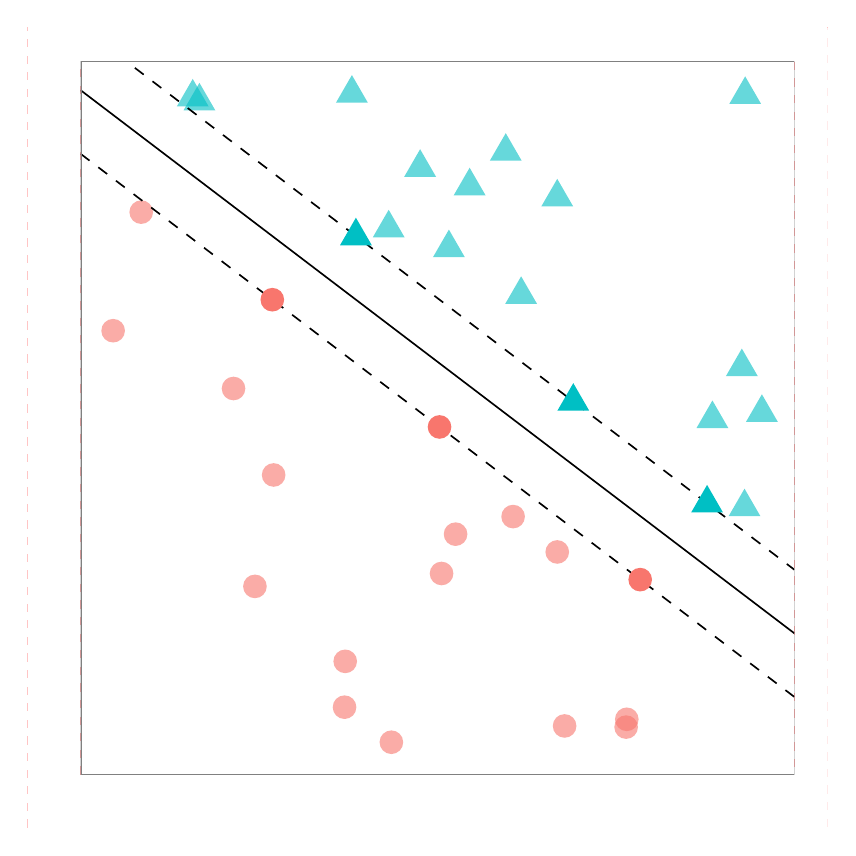
\begin{tikzpicture}[x=1pt,y=1pt]
\definecolor{fillColor}{RGB}{255,255,255}
\path[use as bounding box,fill=fillColor,fill opacity=0.00] (0,0) rectangle (289.08,289.08);
\begin{scope}
\path[clip] (  0.00,  0.00) rectangle (289.08,289.08);
\path[draw=red,very thick,dashed] (  0.00,  0.00) rectangle (289.08,289.08);
\definecolor{drawColor}{RGB}{255,255,255}
\definecolor{fillColor}{RGB}{255,255,255}

\path[draw=drawColor,line width= 0.6pt,line join=round,line cap=round,fill=fillColor] ( -0.00,  0.00) rectangle (289.08,289.08);
\end{scope}
% Drawing Rectangle from x0 = 19.158189, y0 = 19.158189 to x1 = 277.035000, y1 = 277.035000
\begin{scope}
\path[clip] ( 19.16, 19.16) rectangle (277.04,277.03);
\path[draw=red,very thick,dashed] ( 19.16, 19.16) rectangle (277.04,277.03);
\definecolor{fillColor}{RGB}{255,255,255}

\path[fill=fillColor] ( 19.16, 19.16) rectangle (277.03,277.03);
% Drawing Circle at x = 154.622062, y = 106.056512, r = 4.267913
\definecolor{fillColor}{RGB}{248,118,109}

\path[fill=fillColor,fill opacity=0.60] (154.62,106.06) circle (  4.27);
% Drawing Circle at x = 175.406885, y = 112.405282, r = 4.267913

\path[fill=fillColor,fill opacity=0.60] (175.41,112.41) circle (  4.27);
% Drawing Circle at x = 191.358028, y = 99.634396, r = 4.267913

\path[fill=fillColor,fill opacity=0.60] (191.36, 99.63) circle (  4.27);
% Drawing Circle at x = 216.251478, y = 36.338631, r = 4.267913

\path[fill=fillColor,fill opacity=0.60] (216.25, 36.34) circle (  4.27);
% Drawing Circle at x = 30.879862, y = 179.575760, r = 4.267913

\path[fill=fillColor,fill opacity=0.60] ( 30.88,179.58) circle (  4.27);
% Drawing Circle at x = 194.016551, y = 36.759871, r = 4.267913

\path[fill=fillColor,fill opacity=0.60] (194.02, 36.76) circle (  4.27);
% Drawing Circle at x = 114.744205, y = 60.099534, r = 4.267913

\path[fill=fillColor,fill opacity=0.60] (114.74, 60.10) circle (  4.27);
% Drawing Circle at x = 149.546698, y = 91.852348, r = 4.267913

\path[fill=fillColor,fill opacity=0.60] (149.55, 91.85) circle (  4.27);
% Drawing Circle at x = 41.030590, y = 222.420523, r = 4.267913

\path[fill=fillColor,fill opacity=0.60] ( 41.03,222.42) circle (  4.27);
% Drawing Circle at x = 131.420400, y = 30.879862, r = 4.267913

\path[fill=fillColor,fill opacity=0.60] (131.42, 30.88) circle (  4.27);
% Drawing Circle at x = 88.884018, y = 127.453968, r = 4.267913

\path[fill=fillColor,fill opacity=0.60] ( 88.88,127.45) circle (  4.27);
% Drawing Circle at x = 114.502521, y = 43.542980, r = 4.267913

\path[fill=fillColor,fill opacity=0.60] (114.50, 43.54) circle (  4.27);
% Drawing Circle at x = 82.116867, y = 87.186336, r = 4.267913

\path[fill=fillColor,fill opacity=0.60] ( 82.12, 87.19) circle (  4.27);
% Drawing Circle at x = 216.493162, y = 39.157305, r = 4.267913

\path[fill=fillColor,fill opacity=0.60] (216.49, 39.16) circle (  4.27);
% Drawing Circle at x = 74.382979, y = 158.685155, r = 4.267913

\path[fill=fillColor,fill opacity=0.60] ( 74.38,158.69) circle (  4.27);
% Starting Polygon
\definecolor{fillColor}{RGB}{0,191,196}

\path[fill=fillColor,fill opacity=0.60] (152.21,216.11) --
	(157.95,206.15) --
	(146.46,206.15) --
	cycle;
% End Polyline
% Starting Polygon

\path[fill=fillColor,fill opacity=0.60] (265.31,156.60) --
	(271.06,146.65) --
	(259.57,146.65) --
	cycle;
% End Polyline
% Starting Polygon

\path[fill=fillColor,fill opacity=0.60] ( 62.06,269.15) --
	( 67.81,259.19) --
	( 56.31,259.19) --
	cycle;
% End Polyline
% Starting Polygon

\path[fill=fillColor,fill opacity=0.60] (259.03,122.50) --
	(264.78,112.54) --
	(253.28,112.54) --
	cycle;
% End Polyline
% Starting Polygon

\path[fill=fillColor,fill opacity=0.60] (172.75,250.96) --
	(178.50,241.01) --
	(167.00,241.01) --
	cycle;
% End Polyline
% Starting Polygon

\path[fill=fillColor,fill opacity=0.60] (247.43,154.37) --
	(253.18,144.41) --
	(241.68,144.41) --
	cycle;
% End Polyline
% Starting Polygon

\path[fill=fillColor,fill opacity=0.60] (259.27,271.48) --
	(265.02,261.52) --
	(253.52,261.52) --
	cycle;
% End Polyline
% Starting Polygon

\path[fill=fillColor,fill opacity=0.60] ( 59.64,270.56) --
	( 65.39,260.61) --
	( 53.89,260.61) --
	cycle;
% End Polyline
% Starting Polygon

\path[fill=fillColor,fill opacity=0.60] (141.81,245.16) --
	(147.56,235.20) --
	(136.06,235.20) --
	cycle;
% End Polyline
% Starting Polygon

\path[fill=fillColor,fill opacity=0.60] (130.45,223.27) --
	(136.20,213.31) --
	(124.71,213.31) --
	cycle;
% End Polyline
% Starting Polygon

\path[fill=fillColor,fill opacity=0.60] (159.70,238.46) --
	(165.45,228.51) --
	(153.95,228.51) --
	cycle;
% End Polyline
% Starting Polygon

\path[fill=fillColor,fill opacity=0.60] (191.36,234.45) --
	(197.11,224.50) --
	(185.61,224.50) --
	cycle;
% End Polyline
% Starting Polygon

\path[fill=fillColor,fill opacity=0.60] (178.31,199.23) --
	(184.06,189.27) --
	(172.56,189.27) --
	cycle;
% End Polyline
% Starting Polygon

\path[fill=fillColor,fill opacity=0.60] (258.06,173.13) --
	(263.81,163.17) --
	(252.31,163.17) --
	cycle;
% End Polyline
% Starting Polygon

\path[fill=fillColor,fill opacity=0.60] (117.16,271.95) --
	(122.91,261.99) --
	(111.41,261.99) --
	cycle;
% End Polyline
% Drawing line from x1 =    19.1582, y1 =   266.4560 to x2 =   277.0350, y2 =    70.2328
\definecolor{drawColor}{RGB}{0,0,0}

\path[draw=drawColor,line width= 0.6pt,line join=round] ( 19.16,266.46) -- (277.04, 70.23);
% Drawing line from x1 =    19.1582, y1 =   243.4683 to x2 =   277.0350, y2 =    47.2451

\path[draw=drawColor,line width= 0.6pt,dash pattern=on 4pt off 4pt ,line join=round] ( 19.16,243.47) -- (277.04, 47.25);
% Drawing line from x1 =    19.6362, y1 =   289.0800 to x2 =   277.0350, y2 =    93.2205

\path[draw=drawColor,line width= 0.6pt,dash pattern=on 4pt off 4pt ,line join=round] ( 19.64,289.08) -- (277.04, 93.22);
% Drawing Circle at x = 88.400650, y = 190.780418, r = 4.267913
\definecolor{fillColor}{RGB}{248,118,109}

\path[fill=fillColor] ( 88.40,190.78) circle (  4.27);
% Drawing Circle at x = 148.821646, y = 144.804975, r = 4.267913

\path[fill=fillColor] (148.82,144.80) circle (  4.27);
% Drawing Circle at x = 221.326842, y = 89.634443, r = 4.267913

\path[fill=fillColor] (221.33, 89.63) circle (  4.27);
% Starting Polygon
\definecolor{fillColor}{RGB}{0,191,196}

\path[fill=fillColor] (118.61,220.41) --
	(124.36,210.45) --
	(112.86,210.45) --
	cycle;
% End Polyline
% Starting Polygon

\path[fill=fillColor] (197.16,160.64) --
	(202.91,150.68) --
	(191.41,150.68) --
	cycle;
% End Polyline
% Starting Polygon

\path[fill=fillColor] (245.50,123.86) --
	(251.24,113.90) --
	(239.75,113.90) --
	cycle;
% End Polyline
% Drawing Rectangle from x0 = 19.158189, y0 = 19.158189 to x1 = 277.035000, y1 = 277.035000
\definecolor{drawColor}{gray}{0.50}

\path[draw=drawColor,line width= 0.6pt,line join=round,line cap=round] ( 19.16, 19.16) rectangle (277.03,277.03);
\end{scope}
\end{tikzpicture}
% Calculated string width 0 times
}	
\end{figure}
\FloatBarrier

\section{Results}

** Review probabilistic measures created

** Start this section with overview of out-of-sample performance

** Separation plots, bar plots of aggregate statistics

\begin{figure}[ht]
	\centering
	% \resizebox{0.7\textwidth}{!}{% Created by tikzDevice version 0.8.1 on 2015-01-10 22:28:13
% !TEX encoding = UTF-8 Unicode
% Calculated string width of 0.7 as 12.263750
% Calculated character metrics. ascent: 6.611760, descent: 0.000000, width: 8.797910
% Calculated string width of 0.8 as 12.263750
% Calculated string width of 0.9 as 12.263750
% Calculated string width of 1.0 as 12.263750
% Calculated string width of 0.7 as 12.263750
% Calculated string width of 0.8 as 12.263750
% Calculated string width of 0.9 as 12.263750
% Calculated string width of 1.0 as 12.263750
% Calculated character metrics. ascent: 8.264620, descent: 0.000000, width: 10.997280
% Calculated string width of Polity (4 Categories) as 87.392600
% Calculated character metrics. ascent: 6.611760, descent: 0.000000, width: 8.797910
% Calculated string width of Monarchy as 41.616790
% Calculated string width of Party as 23.354450
% Calculated string width of Military as 34.151890
% Calculated character metrics. ascent: 8.264620, descent: 0.000000, width: 10.997280
% Calculated string width of Polity (4 Categories) as 87.392600
% Calculated character metrics. ascent: 6.611760, descent: 0.000000, width: 8.797910
% Calculated string width of Monarchy as 41.616790
% Calculated string width of Party as 23.354450
% Calculated string width of Military as 34.151890
% Calculated string width of Precision as 38.070970
% Calculated string width of Recall as 25.727220
% Calculated string width of F-1 Score as 39.883870
% Calculated string width of Accuracy as 38.684140
% Calculated character metrics. ascent: 8.264620, descent: 0.000000, width: 10.997280
% Drawing Rectangle from x0 = 0.000000, y0 = 0.000000 to x1 = 505.890000, y1 = 361.350000
% Beginning new tikzpicture 'page'
\begin{tikzpicture}[x=1pt,y=1pt]
\definecolor{fillColor}{RGB}{255,255,255}
\path[use as bounding box,fill=fillColor,fill opacity=0.00] (0,0) rectangle (505.89,361.35);
\begin{scope}
\path[clip] (  0.00,  0.00) rectangle (505.89,361.35);
\path[draw=red,very thick,dashed] (  0.00,  0.00) rectangle (505.89,361.35);
\definecolor{drawColor}{RGB}{255,255,255}
\definecolor{fillColor}{RGB}{255,255,255}

\path[draw=drawColor,line width= 0.6pt,line join=round,line cap=round,fill=fillColor] (  0.00,  0.00) rectangle (505.89,361.35);
\end{scope}
% Drawing Rectangle from x0 = 114.815409, y0 = 34.034569 to x1 = 493.845000, y1 = 298.354362
\begin{scope}
\path[clip] (114.82, 34.03) rectangle (493.85,298.35);
\path[draw=red,very thick,dashed] (114.82, 34.03) rectangle (493.85,298.35);
\definecolor{fillColor}{RGB}{255,255,255}

\path[fill=fillColor] (114.82, 34.03) rectangle (493.85,298.35);
% Drawing Rectangle from x0 = 114.815409, y0 = 34.034569 to x1 = 209.572807, y1 = 100.114517
\definecolor{drawColor}{RGB}{255,255,255}
\definecolor{fillColor}{RGB}{97,143,198}

\path[draw=drawColor,line width= 0.1pt,line join=round,fill=fillColor] (114.82, 34.03) rectangle (209.57,100.11);
% Drawing Rectangle from x0 = 114.815409, y0 = 100.114517 to x1 = 209.572807, y1 = 166.194466
\definecolor{fillColor}{RGB}{32,113,180}

\path[draw=drawColor,line width= 0.1pt,line join=round,fill=fillColor] (114.82,100.11) rectangle (209.57,166.19);
% Drawing Rectangle from x0 = 114.815409, y0 = 166.194466 to x1 = 209.572807, y1 = 232.274414

\path[draw=drawColor,line width= 0.1pt,line join=round,fill=fillColor] (114.82,166.19) rectangle (209.57,232.27);
% Drawing Rectangle from x0 = 114.815409, y0 = 232.274414 to x1 = 209.572807, y1 = 298.354362

\path[draw=drawColor,line width= 0.1pt,line join=round,fill=fillColor] (114.82,232.27) rectangle (209.57,298.35);
% Drawing Rectangle from x0 = 209.572807, y0 = 34.034569 to x1 = 304.330204, y1 = 100.114517
\definecolor{fillColor}{RGB}{98,144,199}

\path[draw=drawColor,line width= 0.1pt,line join=round,fill=fillColor] (209.57, 34.03) rectangle (304.33,100.11);
% Drawing Rectangle from x0 = 209.572807, y0 = 100.114517 to x1 = 304.330204, y1 = 166.194466
\definecolor{fillColor}{RGB}{84,135,194}

\path[draw=drawColor,line width= 0.1pt,line join=round,fill=fillColor] (209.57,100.11) rectangle (304.33,166.19);
% Drawing Rectangle from x0 = 209.572807, y0 = 166.194466 to x1 = 304.330204, y1 = 232.274414
\definecolor{fillColor}{RGB}{81,134,193}

\path[draw=drawColor,line width= 0.1pt,line join=round,fill=fillColor] (209.57,166.19) rectangle (304.33,232.27);
% Drawing Rectangle from x0 = 209.572807, y0 = 232.274414 to x1 = 304.330204, y1 = 298.354362
\definecolor{fillColor}{RGB}{197,218,238}

\path[draw=drawColor,line width= 0.1pt,line join=round,fill=fillColor] (209.57,232.27) rectangle (304.33,298.35);
% Drawing Rectangle from x0 = 304.330204, y0 = 34.034569 to x1 = 399.087602, y1 = 100.114517
\definecolor{fillColor}{RGB}{103,147,201}

\path[draw=drawColor,line width= 0.1pt,line join=round,fill=fillColor] (304.33, 34.03) rectangle (399.09,100.11);
% Drawing Rectangle from x0 = 304.330204, y0 = 100.114517 to x1 = 399.087602, y1 = 166.194466
\definecolor{fillColor}{RGB}{63,124,187}

\path[draw=drawColor,line width= 0.1pt,line join=round,fill=fillColor] (304.33,100.11) rectangle (399.09,166.19);
% Drawing Rectangle from x0 = 304.330204, y0 = 166.194466 to x1 = 399.087602, y1 = 232.274414
\definecolor{fillColor}{RGB}{62,124,187}

\path[draw=drawColor,line width= 0.1pt,line join=round,fill=fillColor] (304.33,166.19) rectangle (399.09,232.27);
% Drawing Rectangle from x0 = 304.330204, y0 = 232.274414 to x1 = 399.087602, y1 = 298.354362
\definecolor{fillColor}{RGB}{141,174,215}

\path[draw=drawColor,line width= 0.1pt,line join=round,fill=fillColor] (304.33,232.27) rectangle (399.09,298.35);
% Drawing Rectangle from x0 = 399.087602, y0 = 34.034569 to x1 = 493.845000, y1 = 100.114517
\definecolor{fillColor}{RGB}{98,144,199}

\path[draw=drawColor,line width= 0.1pt,line join=round,fill=fillColor] (399.09, 34.03) rectangle (493.84,100.11);
% Drawing Rectangle from x0 = 399.087602, y0 = 100.114517 to x1 = 493.845000, y1 = 166.194466
\definecolor{fillColor}{RGB}{36,113,181}

\path[draw=drawColor,line width= 0.1pt,line join=round,fill=fillColor] (399.09,100.11) rectangle (493.84,166.19);
% Drawing Rectangle from x0 = 399.087602, y0 = 166.194466 to x1 = 493.845000, y1 = 232.274414

\path[draw=drawColor,line width= 0.1pt,line join=round,fill=fillColor] (399.09,166.19) rectangle (493.84,232.27);
% Drawing Rectangle from x0 = 399.087602, y0 = 232.274414 to x1 = 493.845000, y1 = 298.354362
\definecolor{fillColor}{RGB}{38,114,181}

\path[draw=drawColor,line width= 0.1pt,line join=round,fill=fillColor] (399.09,232.27) rectangle (493.84,298.35);
\end{scope}
% Calculated string width of Polity (4 Categories) as 87.392600
% Calculated character metrics. ascent: 6.611760, descent: 0.000000, width: 8.797910
% Calculated string width of Monarchy as 41.616790
% Calculated string width of Party as 23.354450
% Calculated string width of Military as 34.151890
% Calculated string width of Polity (4 Categories) as 87.392600
% Calculated string width of Monarchy as 41.616790
% Calculated string width of Party as 23.354450
% Calculated string width of Military as 34.151890
% Calculated string width of Polity (4 Categories) as 87.392600
% Calculated string width of Monarchy as 41.616790
% Calculated string width of Party as 23.354450
% Calculated string width of Military as 34.151890
% Calculated string width of Polity (4 Categories) as 87.392600
% Drawing node at x = 107.702220, y = 63.768663
\begin{scope}
\path[clip] (  0.00,  0.00) rectangle (505.89,361.35);
\path[draw=red,very thick,dashed] (  0.00,  0.00) rectangle (505.89,361.35);
\definecolor{drawColor}{RGB}{0,0,0}

\node[text=drawColor,anchor=base east,inner sep=0pt, outer sep=0pt, scale=  0.96] at (107.70, 63.77) {Polity (4 Categories)};

\draw[color=red, fill=red] (107.70, 63.77) circle (0.5pt);
% Calculated string width of Monarchy as 41.616790
% Drawing node at x = 107.702220, y = 129.848611

\node[text=drawColor,anchor=base east,inner sep=0pt, outer sep=0pt, scale=  0.96] at (107.70,129.85) {Monarchy};

\draw[color=red, fill=red] (107.70,129.85) circle (0.5pt);
% Calculated string width of Party as 23.354450
% Drawing node at x = 107.702220, y = 195.928560

\node[text=drawColor,anchor=base east,inner sep=0pt, outer sep=0pt, scale=  0.96] at (107.70,195.93) {Party};

\draw[color=red, fill=red] (107.70,195.93) circle (0.5pt);
% Calculated string width of Military as 34.151890
% Drawing node at x = 107.702220, y = 262.008508

\node[text=drawColor,anchor=base east,inner sep=0pt, outer sep=0pt, scale=  0.96] at (107.70,262.01) {Military};

\draw[color=red, fill=red] (107.70,262.01) circle (0.5pt);
\end{scope}
% Calculated string width of Precision as 38.070970
% Calculated string width of Recall as 25.727220
% Calculated string width of F-1 Score as 39.883870
% Calculated string width of Accuracy as 38.684140
% Calculated string width of Precision as 38.070970
% Calculated string width of Recall as 25.727220
% Calculated string width of F-1 Score as 39.883870
% Calculated string width of Accuracy as 38.684140
% Calculated string width of Precision as 38.070970
% Calculated string width of Recall as 25.727220
% Calculated string width of F-1 Score as 39.883870
% Calculated string width of Accuracy as 38.684140
% Calculated string width of Precision as 38.070970
% Drawing node at x = 162.194108, y = 20.309620
\begin{scope}
\path[clip] (  0.00,  0.00) rectangle (505.89,361.35);
\path[draw=red,very thick,dashed] (  0.00,  0.00) rectangle (505.89,361.35);
\definecolor{drawColor}{RGB}{0,0,0}

\node[text=drawColor,anchor=base,inner sep=0pt, outer sep=0pt, scale=  0.96] at (162.19, 20.31) {Precision};

\draw[color=red, fill=red] (162.19, 20.31) circle (0.5pt);
% Calculated string width of Recall as 25.727220
% Drawing node at x = 256.951506, y = 20.309620

\node[text=drawColor,anchor=base,inner sep=0pt, outer sep=0pt, scale=  0.96] at (256.95, 20.31) {Recall};

\draw[color=red, fill=red] (256.95, 20.31) circle (0.5pt);
% Calculated string width of F-1 Score as 39.883870
% Drawing node at x = 351.708903, y = 20.309620

\node[text=drawColor,anchor=base,inner sep=0pt, outer sep=0pt, scale=  0.96] at (351.71, 20.31) {F-1 Score};

\draw[color=red, fill=red] (351.71, 20.31) circle (0.5pt);
% Calculated string width of Accuracy as 38.684140
% Drawing node at x = 446.466301, y = 20.309620

\node[text=drawColor,anchor=base,inner sep=0pt, outer sep=0pt, scale=  0.96] at (446.47, 20.31) {Accuracy};

\draw[color=red, fill=red] (446.47, 20.31) circle (0.5pt);
\end{scope}
% Drawing Rectangle from x0 = 155.991762, y0 = 307.222138 to x1 = 452.668647, y1 = 340.437224
\begin{scope}
\path[clip] (  0.00,  0.00) rectangle (505.89,361.35);
\path[draw=red,very thick,dashed] (  0.00,  0.00) rectangle (505.89,361.35);
\definecolor{fillColor}{RGB}{255,255,255}

\path[fill=fillColor] (155.99,307.22) rectangle (452.67,340.44);
\end{scope}
\begin{scope}
\path[clip] (  0.00,  0.00) rectangle (505.89,361.35);
\path[draw=red,very thick,dashed] (  0.00,  0.00) rectangle (505.89,361.35);
\node[inner sep=0pt,outer sep=0pt,anchor=south west,rotate=  0.00] at (163.87, 321.72) {
	\pgfimage[width=284.53pt,height= 14.45pt,interpolate=true]{allAggPerf_ras1}};
\draw[fill=red] (163.87, 321.72) circle (1pt);\end{scope}
% Calculated string width of 0.7 as 12.263750
% Drawing node at x = 187.880188, y = 311.490051
\begin{scope}
\path[clip] (  0.00,  0.00) rectangle (505.89,361.35);
\path[draw=red,very thick,dashed] (  0.00,  0.00) rectangle (505.89,361.35);
\definecolor{drawColor}{RGB}{0,0,0}

\node[text=drawColor,anchor=base,inner sep=0pt, outer sep=0pt, scale=  0.96] at (187.88,311.49) {0.7};

\draw[color=red, fill=red] (187.88,311.49) circle (0.5pt);
% Calculated string width of 0.8 as 12.263750
% Drawing node at x = 272.349307, y = 311.490051

\node[text=drawColor,anchor=base,inner sep=0pt, outer sep=0pt, scale=  0.96] at (272.35,311.49) {0.8};

\draw[color=red, fill=red] (272.35,311.49) circle (0.5pt);
% Calculated string width of 0.9 as 12.263750
% Drawing node at x = 356.818426, y = 311.490051

\node[text=drawColor,anchor=base,inner sep=0pt, outer sep=0pt, scale=  0.96] at (356.82,311.49) {0.9};

\draw[color=red, fill=red] (356.82,311.49) circle (0.5pt);
% Calculated string width of 1.0 as 12.263750
% Drawing node at x = 441.287545, y = 311.490051

\node[text=drawColor,anchor=base,inner sep=0pt, outer sep=0pt, scale=  0.96] at (441.29,311.49) {1.0};

\draw[color=red, fill=red] (441.29,311.49) circle (0.5pt);
\end{scope}
% Drawing line from x1 =   187.8802, y1 =   321.7153 to x2 =   187.8802, y2 =   324.6061
\begin{scope}
\path[clip] (  0.00,  0.00) rectangle (505.89,361.35);
\path[draw=red,very thick,dashed] (  0.00,  0.00) rectangle (505.89,361.35);
\definecolor{drawColor}{RGB}{255,255,255}

\path[draw=drawColor,line width= 0.2pt,line join=round] (187.88,321.72) -- (187.88,324.61);
% Drawing line from x1 =   272.3493, y1 =   321.7153 to x2 =   272.3493, y2 =   324.6061

\path[draw=drawColor,line width= 0.2pt,line join=round] (272.35,321.72) -- (272.35,324.61);
% Drawing line from x1 =   356.8184, y1 =   321.7153 to x2 =   356.8184, y2 =   324.6061

\path[draw=drawColor,line width= 0.2pt,line join=round] (356.82,321.72) -- (356.82,324.61);
% Drawing line from x1 =   441.2875, y1 =   321.7153 to x2 =   441.2875, y2 =   324.6061

\path[draw=drawColor,line width= 0.2pt,line join=round] (441.29,321.72) -- (441.29,324.61);
% Drawing line from x1 =   187.8802, y1 =   333.2785 to x2 =   187.8802, y2 =   336.1693

\path[draw=drawColor,line width= 0.2pt,line join=round] (187.88,333.28) -- (187.88,336.17);
% Drawing line from x1 =   272.3493, y1 =   333.2785 to x2 =   272.3493, y2 =   336.1693

\path[draw=drawColor,line width= 0.2pt,line join=round] (272.35,333.28) -- (272.35,336.17);
% Drawing line from x1 =   356.8184, y1 =   333.2785 to x2 =   356.8184, y2 =   336.1693

\path[draw=drawColor,line width= 0.2pt,line join=round] (356.82,333.28) -- (356.82,336.17);
% Drawing line from x1 =   441.2875, y1 =   333.2785 to x2 =   441.2875, y2 =   336.1693

\path[draw=drawColor,line width= 0.2pt,line join=round] (441.29,333.28) -- (441.29,336.17);
\end{scope}
\end{tikzpicture}
% Calculated string width 56 times
}
	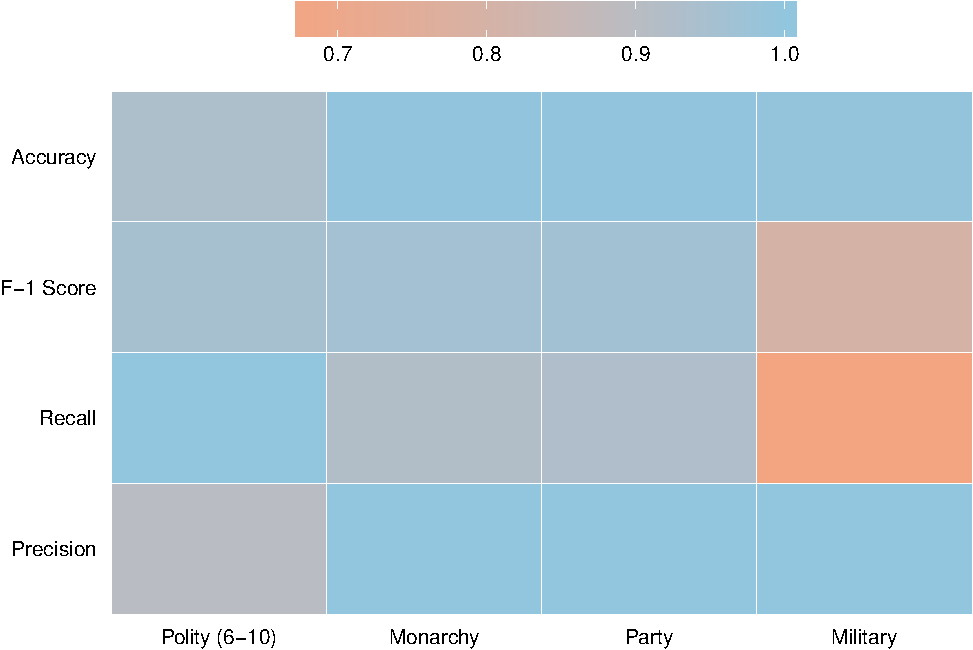
\includegraphics[width=.7\textwidth]{allAggPerf}	
\end{figure}
\FloatBarrier

\begin{figure}[ht]
	\centering
	% \resizebox{0.7\textwidth}{!}{% Created by tikzDevice version 0.8.1 on 2015-01-10 22:28:22
% !TEX encoding = UTF-8 Unicode
% Calculated string width of 1 as 4.798860
% Calculated character metrics. ascent: 6.611760, descent: 0.000000, width: 8.797910
% Calculated string width of 2 as 4.798860
% Calculated string width of 3 as 4.798860
% Calculated string width of 4 as 4.798860
% Calculated string width of 0 as 4.798860
% Calculated string width of 1 as 4.798860
% Calculated string width of 0 as 4.798860
% Calculated string width of 1 as 4.798860
% Calculated string width of 0 as 4.798860
% Calculated string width of 1 as 4.798860
% Calculated string width of Polity (4 Categories) as 87.392600
% Calculated string width of Monarchy as 41.616790
% Calculated string width of Party as 23.354450
% Calculated string width of Military as 34.151890
% Calculated string width of Precision as 38.070970
% Calculated string width of Recall as 25.727220
% Calculated string width of F-1 Score as 39.883870
% Calculated string width of Precision as 38.070970
% Calculated string width of Recall as 25.727220
% Calculated string width of F-1 Score as 39.883870
% Calculated string width of 0.5 as 12.263750
% Calculated string width of 0.6 as 12.263750
% Calculated string width of 0.7 as 12.263750
% Calculated string width of 0.8 as 12.263750
% Calculated string width of 0.9 as 12.263750
% Calculated string width of 1.0 as 12.263750
% Calculated string width of 0.5 as 12.263750
% Calculated string width of 0.6 as 12.263750
% Calculated string width of 0.7 as 12.263750
% Calculated string width of 0.8 as 12.263750
% Calculated string width of 0.9 as 12.263750
% Calculated string width of 1.0 as 12.263750
% Calculated character metrics. ascent: 8.264620, descent: 0.000000, width: 10.997280
% Drawing Rectangle from x0 = 0.000000, y0 = 0.000000 to x1 = 505.890000, y1 = 361.350000
% Beginning new tikzpicture 'page'
\begin{tikzpicture}[x=1pt,y=1pt]
\definecolor{fillColor}{RGB}{255,255,255}
\path[use as bounding box,fill=fillColor,fill opacity=0.00] (0,0) rectangle (505.89,361.35);
\begin{scope}
\path[clip] (  0.00,  0.00) rectangle (505.89,361.35);
\path[draw=red,very thick,dashed] (  0.00,  0.00) rectangle (505.89,361.35);
\definecolor{drawColor}{RGB}{255,255,255}
\definecolor{fillColor}{RGB}{255,255,255}

\path[draw=drawColor,line width= 0.6pt,line join=round,line cap=round,fill=fillColor] (  0.00,  0.00) rectangle (505.89,361.35);
\end{scope}
% Drawing Rectangle from x0 = 32.221669, y0 = 167.700091 to x1 = 255.571685, y1 = 285.720102
\begin{scope}
\path[clip] ( 32.22,167.70) rectangle (255.57,285.72);
\path[draw=red,very thick,dashed] ( 32.22,167.70) rectangle (255.57,285.72);
\definecolor{fillColor}{RGB}{255,255,255}

\path[fill=fillColor] ( 32.22,167.70) rectangle (255.57,285.72);
% Drawing Rectangle from x0 = 32.221669, y0 = 167.700091 to x1 = 106.671674, y1 = 197.205093
\definecolor{drawColor}{RGB}{255,255,255}
\definecolor{fillColor}{RGB}{69,127,189}

\path[draw=drawColor,line width= 0.1pt,line join=round,fill=fillColor] ( 32.22,167.70) rectangle (106.67,197.21);
% Drawing Rectangle from x0 = 32.221669, y0 = 197.205093 to x1 = 106.671674, y1 = 226.710096
\definecolor{fillColor}{RGB}{92,140,197}

\path[draw=drawColor,line width= 0.1pt,line join=round,fill=fillColor] ( 32.22,197.21) rectangle (106.67,226.71);
% Drawing Rectangle from x0 = 32.221669, y0 = 226.710096 to x1 = 106.671674, y1 = 256.215099
\definecolor{fillColor}{RGB}{72,129,190}

\path[draw=drawColor,line width= 0.1pt,line join=round,fill=fillColor] ( 32.22,226.71) rectangle (106.67,256.22);
% Drawing Rectangle from x0 = 32.221669, y0 = 256.215099 to x1 = 106.671674, y1 = 285.720102
\definecolor{fillColor}{RGB}{76,131,191}

\path[draw=drawColor,line width= 0.1pt,line join=round,fill=fillColor] ( 32.22,256.22) rectangle (106.67,285.72);
% Drawing Rectangle from x0 = 106.671674, y0 = 167.700091 to x1 = 181.121680, y1 = 197.205093
\definecolor{fillColor}{RGB}{38,114,182}

\path[draw=drawColor,line width= 0.1pt,line join=round,fill=fillColor] (106.67,167.70) rectangle (181.12,197.21);
% Drawing Rectangle from x0 = 106.671674, y0 = 197.205093 to x1 = 181.121680, y1 = 226.710096
\definecolor{fillColor}{RGB}{98,144,199}

\path[draw=drawColor,line width= 0.1pt,line join=round,fill=fillColor] (106.67,197.21) rectangle (181.12,226.71);
% Drawing Rectangle from x0 = 106.671674, y0 = 226.710096 to x1 = 181.121680, y1 = 256.215099
\definecolor{fillColor}{RGB}{197,218,238}

\path[draw=drawColor,line width= 0.1pt,line join=round,fill=fillColor] (106.67,226.71) rectangle (181.12,256.22);
% Drawing Rectangle from x0 = 106.671674, y0 = 256.215099 to x1 = 181.121680, y1 = 285.720102
\definecolor{fillColor}{RGB}{32,113,180}

\path[draw=drawColor,line width= 0.1pt,line join=round,fill=fillColor] (106.67,256.22) rectangle (181.12,285.72);
% Drawing Rectangle from x0 = 181.121680, y0 = 167.700091 to x1 = 255.571685, y1 = 197.205093
\definecolor{fillColor}{RGB}{57,122,186}

\path[draw=drawColor,line width= 0.1pt,line join=round,fill=fillColor] (181.12,167.70) rectangle (255.57,197.21);
% Drawing Rectangle from x0 = 181.121680, y0 = 197.205093 to x1 = 255.571685, y1 = 226.710096
\definecolor{fillColor}{RGB}{95,142,198}

\path[draw=drawColor,line width= 0.1pt,line join=round,fill=fillColor] (181.12,197.21) rectangle (255.57,226.71);
% Drawing Rectangle from x0 = 181.121680, y0 = 226.710096 to x1 = 255.571685, y1 = 256.215099
\definecolor{fillColor}{RGB}{159,188,222}

\path[draw=drawColor,line width= 0.1pt,line join=round,fill=fillColor] (181.12,226.71) rectangle (255.57,256.22);
% Drawing Rectangle from x0 = 181.121680, y0 = 256.215099 to x1 = 255.571685, y1 = 285.720102
\definecolor{fillColor}{RGB}{57,122,186}

\path[draw=drawColor,line width= 0.1pt,line join=round,fill=fillColor] (181.12,256.22) rectangle (255.57,285.72);
\end{scope}
% Drawing Rectangle from x0 = 270.494984, y0 = 167.700091 to x1 = 493.845000, y1 = 285.720102
\begin{scope}
\path[clip] (270.49,167.70) rectangle (493.85,285.72);
\path[draw=red,very thick,dashed] (270.49,167.70) rectangle (493.85,285.72);
\definecolor{fillColor}{RGB}{255,255,255}

\path[fill=fillColor] (270.49,167.70) rectangle (493.85,285.72);
% Drawing Rectangle from x0 = 270.494984, y0 = 167.700091 to x1 = 344.944989, y1 = 226.710096
\definecolor{drawColor}{RGB}{255,255,255}
\definecolor{fillColor}{RGB}{32,113,180}

\path[draw=drawColor,line width= 0.1pt,line join=round,fill=fillColor] (270.49,167.70) rectangle (344.94,226.71);
% Drawing Rectangle from x0 = 270.494984, y0 = 226.710096 to x1 = 344.944989, y1 = 285.720102

\path[draw=drawColor,line width= 0.1pt,line join=round,fill=fillColor] (270.49,226.71) rectangle (344.94,285.72);
% Drawing Rectangle from x0 = 344.944989, y0 = 167.700091 to x1 = 419.394995, y1 = 226.710096

\path[draw=drawColor,line width= 0.1pt,line join=round,fill=fillColor] (344.94,167.70) rectangle (419.39,226.71);
% Drawing Rectangle from x0 = 344.944989, y0 = 226.710096 to x1 = 419.394995, y1 = 285.720102
\definecolor{fillColor}{RGB}{69,127,189}

\path[draw=drawColor,line width= 0.1pt,line join=round,fill=fillColor] (344.94,226.71) rectangle (419.39,285.72);
% Drawing Rectangle from x0 = 419.394995, y0 = 167.700091 to x1 = 493.845000, y1 = 226.710096
\definecolor{fillColor}{RGB}{32,113,180}

\path[draw=drawColor,line width= 0.1pt,line join=round,fill=fillColor] (419.39,167.70) rectangle (493.85,226.71);
% Drawing Rectangle from x0 = 419.394995, y0 = 226.710096 to x1 = 493.845000, y1 = 285.720102
\definecolor{fillColor}{RGB}{53,120,185}

\path[draw=drawColor,line width= 0.1pt,line join=round,fill=fillColor] (419.39,226.71) rectangle (493.85,285.72);
\end{scope}
% Drawing Rectangle from x0 = 32.221669, y0 = 34.034569 to x1 = 255.571685, y1 = 152.054581
\begin{scope}
\path[clip] ( 32.22, 34.03) rectangle (255.57,152.05);
\path[draw=red,very thick,dashed] ( 32.22, 34.03) rectangle (255.57,152.05);
\definecolor{fillColor}{RGB}{255,255,255}

\path[fill=fillColor] ( 32.22, 34.03) rectangle (255.57,152.05);
% Drawing Rectangle from x0 = 32.221669, y0 = 34.034569 to x1 = 106.671674, y1 = 93.044575
\definecolor{drawColor}{RGB}{255,255,255}
\definecolor{fillColor}{RGB}{32,113,180}

\path[draw=drawColor,line width= 0.1pt,line join=round,fill=fillColor] ( 32.22, 34.03) rectangle (106.67, 93.04);
% Drawing Rectangle from x0 = 32.221669, y0 = 93.044575 to x1 = 106.671674, y1 = 152.054581

\path[draw=drawColor,line width= 0.1pt,line join=round,fill=fillColor] ( 32.22, 93.04) rectangle (106.67,152.05);
% Drawing Rectangle from x0 = 106.671674, y0 = 34.034569 to x1 = 181.121680, y1 = 93.044575

\path[draw=drawColor,line width= 0.1pt,line join=round,fill=fillColor] (106.67, 34.03) rectangle (181.12, 93.04);
% Drawing Rectangle from x0 = 106.671674, y0 = 93.044575 to x1 = 181.121680, y1 = 152.054581
\definecolor{fillColor}{RGB}{65,125,188}

\path[draw=drawColor,line width= 0.1pt,line join=round,fill=fillColor] (106.67, 93.04) rectangle (181.12,152.05);
% Drawing Rectangle from x0 = 181.121680, y0 = 34.034569 to x1 = 255.571685, y1 = 93.044575
\definecolor{fillColor}{RGB}{32,113,180}

\path[draw=drawColor,line width= 0.1pt,line join=round,fill=fillColor] (181.12, 34.03) rectangle (255.57, 93.04);
% Drawing Rectangle from x0 = 181.121680, y0 = 93.044575 to x1 = 255.571685, y1 = 152.054581
\definecolor{fillColor}{RGB}{53,120,185}

\path[draw=drawColor,line width= 0.1pt,line join=round,fill=fillColor] (181.12, 93.04) rectangle (255.57,152.05);
\end{scope}
% Drawing Rectangle from x0 = 270.494984, y0 = 34.034569 to x1 = 493.845000, y1 = 152.054581
\begin{scope}
\path[clip] (270.49, 34.03) rectangle (493.85,152.05);
\path[draw=red,very thick,dashed] (270.49, 34.03) rectangle (493.85,152.05);
\definecolor{fillColor}{RGB}{255,255,255}

\path[fill=fillColor] (270.49, 34.03) rectangle (493.85,152.05);
% Drawing Rectangle from x0 = 270.494984, y0 = 34.034569 to x1 = 344.944989, y1 = 93.044575
\definecolor{drawColor}{RGB}{255,255,255}
\definecolor{fillColor}{RGB}{38,114,182}

\path[draw=drawColor,line width= 0.1pt,line join=round,fill=fillColor] (270.49, 34.03) rectangle (344.94, 93.04);
% Drawing Rectangle from x0 = 270.494984, y0 = 93.044575 to x1 = 344.944989, y1 = 152.054581
\definecolor{fillColor}{RGB}{32,113,180}

\path[draw=drawColor,line width= 0.1pt,line join=round,fill=fillColor] (270.49, 93.04) rectangle (344.94,152.05);
% Drawing Rectangle from x0 = 344.944989, y0 = 34.034569 to x1 = 419.394995, y1 = 93.044575

\path[draw=drawColor,line width= 0.1pt,line join=round,fill=fillColor] (344.94, 34.03) rectangle (419.39, 93.04);
% Drawing Rectangle from x0 = 344.944989, y0 = 93.044575 to x1 = 419.394995, y1 = 152.054581
\definecolor{fillColor}{RGB}{143,176,216}

\path[draw=drawColor,line width= 0.1pt,line join=round,fill=fillColor] (344.94, 93.04) rectangle (419.39,152.05);
% Drawing Rectangle from x0 = 419.394995, y0 = 34.034569 to x1 = 493.845000, y1 = 93.044575
\definecolor{fillColor}{RGB}{32,113,180}

\path[draw=drawColor,line width= 0.1pt,line join=round,fill=fillColor] (419.39, 34.03) rectangle (493.85, 93.04);
% Drawing Rectangle from x0 = 419.394995, y0 = 93.044575 to x1 = 493.845000, y1 = 152.054581
\definecolor{fillColor}{RGB}{107,150,202}

\path[draw=drawColor,line width= 0.1pt,line join=round,fill=fillColor] (419.39, 93.04) rectangle (493.85,152.05);
\end{scope}
% Drawing Rectangle from x0 = 32.221669, y0 = 285.720102 to x1 = 255.571685, y1 = 298.354362
\begin{scope}
\path[clip] (  0.00,  0.00) rectangle (505.89,361.35);
\path[draw=red,very thick,dashed] (  0.00,  0.00) rectangle (505.89,361.35);
\definecolor{drawColor}{gray}{0.50}
\definecolor{fillColor}{gray}{0.80}

\path[draw=drawColor,line width= 0.2pt,line join=round,line cap=round,fill=fillColor] ( 32.22,285.72) rectangle (255.57,298.35);
% Calculated string width of Polity (4 Categories) as 87.392600
% Calculated character metrics. ascent: 6.611760, descent: 0.000000, width: 8.797910
% Drawing node at x = 143.896677, y = 288.731352
\definecolor{drawColor}{RGB}{0,0,0}

\node[text=drawColor,anchor=base,inner sep=0pt, outer sep=0pt, scale=  0.96] at (143.90,288.73) {Polity (4 Categories)};

\draw[color=red, fill=red] (143.90,288.73) circle (0.5pt);
\end{scope}
% Drawing Rectangle from x0 = 270.494984, y0 = 285.720102 to x1 = 493.845000, y1 = 298.354362
\begin{scope}
\path[clip] (  0.00,  0.00) rectangle (505.89,361.35);
\path[draw=red,very thick,dashed] (  0.00,  0.00) rectangle (505.89,361.35);
\definecolor{drawColor}{gray}{0.50}
\definecolor{fillColor}{gray}{0.80}

\path[draw=drawColor,line width= 0.2pt,line join=round,line cap=round,fill=fillColor] (270.49,285.72) rectangle (493.85,298.35);
% Calculated string width of Monarchy as 41.616790
% Drawing node at x = 382.169992, y = 288.731352
\definecolor{drawColor}{RGB}{0,0,0}

\node[text=drawColor,anchor=base,inner sep=0pt, outer sep=0pt, scale=  0.96] at (382.17,288.73) {Monarchy};

\draw[color=red, fill=red] (382.17,288.73) circle (0.5pt);
\end{scope}
% Drawing Rectangle from x0 = 32.221669, y0 = 152.054581 to x1 = 255.571685, y1 = 164.688841
\begin{scope}
\path[clip] (  0.00,  0.00) rectangle (505.89,361.35);
\path[draw=red,very thick,dashed] (  0.00,  0.00) rectangle (505.89,361.35);
\definecolor{drawColor}{gray}{0.50}
\definecolor{fillColor}{gray}{0.80}

\path[draw=drawColor,line width= 0.2pt,line join=round,line cap=round,fill=fillColor] ( 32.22,152.05) rectangle (255.57,164.69);
% Calculated string width of Party as 23.354450
% Drawing node at x = 143.896677, y = 155.065831
\definecolor{drawColor}{RGB}{0,0,0}

\node[text=drawColor,anchor=base,inner sep=0pt, outer sep=0pt, scale=  0.96] at (143.90,155.07) {Party};

\draw[color=red, fill=red] (143.90,155.07) circle (0.5pt);
\end{scope}
% Drawing Rectangle from x0 = 270.494984, y0 = 152.054581 to x1 = 493.845000, y1 = 164.688841
\begin{scope}
\path[clip] (  0.00,  0.00) rectangle (505.89,361.35);
\path[draw=red,very thick,dashed] (  0.00,  0.00) rectangle (505.89,361.35);
\definecolor{drawColor}{gray}{0.50}
\definecolor{fillColor}{gray}{0.80}

\path[draw=drawColor,line width= 0.2pt,line join=round,line cap=round,fill=fillColor] (270.49,152.05) rectangle (493.85,164.69);
% Calculated string width of Military as 34.151890
% Drawing node at x = 382.169992, y = 155.065831
\definecolor{drawColor}{RGB}{0,0,0}

\node[text=drawColor,anchor=base,inner sep=0pt, outer sep=0pt, scale=  0.96] at (382.17,155.07) {Military};

\draw[color=red, fill=red] (382.17,155.07) circle (0.5pt);
\end{scope}
% Calculated string width of 1 as 4.798860
% Calculated string width of 2 as 4.798860
% Calculated string width of 3 as 4.798860
% Calculated string width of 4 as 4.798860
% Calculated string width of 1 as 4.798860
% Calculated string width of 2 as 4.798860
% Calculated string width of 3 as 4.798860
% Calculated string width of 4 as 4.798860
% Calculated string width of 1 as 4.798860
% Calculated string width of 2 as 4.798860
% Calculated string width of 3 as 4.798860
% Calculated string width of 4 as 4.798860
% Calculated string width of 1 as 4.798860
% Drawing node at x = 25.108480, y = 179.146712
\begin{scope}
\path[clip] (  0.00,  0.00) rectangle (505.89,361.35);
\path[draw=red,very thick,dashed] (  0.00,  0.00) rectangle (505.89,361.35);
\definecolor{drawColor}{RGB}{0,0,0}

\node[text=drawColor,anchor=base east,inner sep=0pt, outer sep=0pt, scale=  0.96] at ( 25.11,179.15) {1};

\draw[color=red, fill=red] ( 25.11,179.15) circle (0.5pt);
% Calculated string width of 2 as 4.798860
% Drawing node at x = 25.108480, y = 208.651715

\node[text=drawColor,anchor=base east,inner sep=0pt, outer sep=0pt, scale=  0.96] at ( 25.11,208.65) {2};

\draw[color=red, fill=red] ( 25.11,208.65) circle (0.5pt);
% Calculated string width of 3 as 4.798860
% Drawing node at x = 25.108480, y = 238.156718

\node[text=drawColor,anchor=base east,inner sep=0pt, outer sep=0pt, scale=  0.96] at ( 25.11,238.16) {3};

\draw[color=red, fill=red] ( 25.11,238.16) circle (0.5pt);
% Calculated string width of 4 as 4.798860
% Drawing node at x = 25.108480, y = 267.661721

\node[text=drawColor,anchor=base east,inner sep=0pt, outer sep=0pt, scale=  0.96] at ( 25.11,267.66) {4};

\draw[color=red, fill=red] ( 25.11,267.66) circle (0.5pt);
\end{scope}
% Calculated string width of 0 as 4.798860
% Calculated string width of 1 as 4.798860
% Calculated string width of 0 as 4.798860
% Calculated string width of 1 as 4.798860
% Calculated string width of 0 as 4.798860
% Calculated string width of 1 as 4.798860
% Calculated string width of 0 as 4.798860
% Drawing node at x = 263.381795, y = 193.899213
\begin{scope}
\path[clip] (  0.00,  0.00) rectangle (505.89,361.35);
\path[draw=red,very thick,dashed] (  0.00,  0.00) rectangle (505.89,361.35);
\definecolor{drawColor}{RGB}{0,0,0}

\node[text=drawColor,anchor=base east,inner sep=0pt, outer sep=0pt, scale=  0.96] at (263.38,193.90) {0};

\draw[color=red, fill=red] (263.38,193.90) circle (0.5pt);
% Calculated string width of 1 as 4.798860
% Drawing node at x = 263.381795, y = 252.909219

\node[text=drawColor,anchor=base east,inner sep=0pt, outer sep=0pt, scale=  0.96] at (263.38,252.91) {1};

\draw[color=red, fill=red] (263.38,252.91) circle (0.5pt);
\end{scope}
% Calculated string width of 0 as 4.798860
% Calculated string width of 1 as 4.798860
% Calculated string width of 0 as 4.798860
% Calculated string width of 1 as 4.798860
% Calculated string width of 0 as 4.798860
% Calculated string width of 1 as 4.798860
% Calculated string width of 0 as 4.798860
% Drawing node at x = 25.108480, y = 60.233692
\begin{scope}
\path[clip] (  0.00,  0.00) rectangle (505.89,361.35);
\path[draw=red,very thick,dashed] (  0.00,  0.00) rectangle (505.89,361.35);
\definecolor{drawColor}{RGB}{0,0,0}

\node[text=drawColor,anchor=base east,inner sep=0pt, outer sep=0pt, scale=  0.96] at ( 25.11, 60.23) {0};

\draw[color=red, fill=red] ( 25.11, 60.23) circle (0.5pt);
% Calculated string width of 1 as 4.798860
% Drawing node at x = 25.108480, y = 119.243698

\node[text=drawColor,anchor=base east,inner sep=0pt, outer sep=0pt, scale=  0.96] at ( 25.11,119.24) {1};

\draw[color=red, fill=red] ( 25.11,119.24) circle (0.5pt);
\end{scope}
% Calculated string width of 0 as 4.798860
% Calculated string width of 1 as 4.798860
% Calculated string width of 0 as 4.798860
% Calculated string width of 1 as 4.798860
% Calculated string width of 0 as 4.798860
% Calculated string width of 1 as 4.798860
% Calculated string width of 0 as 4.798860
% Drawing node at x = 263.381795, y = 60.233692
\begin{scope}
\path[clip] (  0.00,  0.00) rectangle (505.89,361.35);
\path[draw=red,very thick,dashed] (  0.00,  0.00) rectangle (505.89,361.35);
\definecolor{drawColor}{RGB}{0,0,0}

\node[text=drawColor,anchor=base east,inner sep=0pt, outer sep=0pt, scale=  0.96] at (263.38, 60.23) {0};

\draw[color=red, fill=red] (263.38, 60.23) circle (0.5pt);
% Calculated string width of 1 as 4.798860
% Drawing node at x = 263.381795, y = 119.243698

\node[text=drawColor,anchor=base east,inner sep=0pt, outer sep=0pt, scale=  0.96] at (263.38,119.24) {1};

\draw[color=red, fill=red] (263.38,119.24) circle (0.5pt);
\end{scope}
% Calculated string width of Precision as 38.070970
% Calculated string width of Recall as 25.727220
% Calculated string width of F-1 Score as 39.883870
% Calculated string width of Precision as 38.070970
% Calculated string width of Recall as 25.727220
% Calculated string width of F-1 Score as 39.883870
% Calculated string width of Precision as 38.070970
% Calculated string width of Recall as 25.727220
% Calculated string width of F-1 Score as 39.883870
% Calculated string width of Precision as 38.070970
% Drawing node at x = 69.446672, y = 20.309620
\begin{scope}
\path[clip] (  0.00,  0.00) rectangle (505.89,361.35);
\path[draw=red,very thick,dashed] (  0.00,  0.00) rectangle (505.89,361.35);
\definecolor{drawColor}{RGB}{0,0,0}

\node[text=drawColor,anchor=base,inner sep=0pt, outer sep=0pt, scale=  0.96] at ( 69.45, 20.31) {Precision};

\draw[color=red, fill=red] ( 69.45, 20.31) circle (0.5pt);
% Calculated string width of Recall as 25.727220
% Drawing node at x = 143.896677, y = 20.309620

\node[text=drawColor,anchor=base,inner sep=0pt, outer sep=0pt, scale=  0.96] at (143.90, 20.31) {Recall};

\draw[color=red, fill=red] (143.90, 20.31) circle (0.5pt);
% Calculated string width of F-1 Score as 39.883870
% Drawing node at x = 218.346682, y = 20.309620

\node[text=drawColor,anchor=base,inner sep=0pt, outer sep=0pt, scale=  0.96] at (218.35, 20.31) {F-1 Score};

\draw[color=red, fill=red] (218.35, 20.31) circle (0.5pt);
\end{scope}
% Calculated string width of Precision as 38.070970
% Calculated string width of Recall as 25.727220
% Calculated string width of F-1 Score as 39.883870
% Calculated string width of Precision as 38.070970
% Calculated string width of Recall as 25.727220
% Calculated string width of F-1 Score as 39.883870
% Calculated string width of Precision as 38.070970
% Calculated string width of Recall as 25.727220
% Calculated string width of F-1 Score as 39.883870
% Calculated string width of Precision as 38.070970
% Drawing node at x = 307.719987, y = 20.309620
\begin{scope}
\path[clip] (  0.00,  0.00) rectangle (505.89,361.35);
\path[draw=red,very thick,dashed] (  0.00,  0.00) rectangle (505.89,361.35);
\definecolor{drawColor}{RGB}{0,0,0}

\node[text=drawColor,anchor=base,inner sep=0pt, outer sep=0pt, scale=  0.96] at (307.72, 20.31) {Precision};

\draw[color=red, fill=red] (307.72, 20.31) circle (0.5pt);
% Calculated string width of Recall as 25.727220
% Drawing node at x = 382.169992, y = 20.309620

\node[text=drawColor,anchor=base,inner sep=0pt, outer sep=0pt, scale=  0.96] at (382.17, 20.31) {Recall};

\draw[color=red, fill=red] (382.17, 20.31) circle (0.5pt);
% Calculated string width of F-1 Score as 39.883870
% Drawing node at x = 456.619997, y = 20.309620

\node[text=drawColor,anchor=base,inner sep=0pt, outer sep=0pt, scale=  0.96] at (456.62, 20.31) {F-1 Score};

\draw[color=red, fill=red] (456.62, 20.31) circle (0.5pt);
\end{scope}
% Drawing Rectangle from x0 = 114.694892, y0 = 307.222138 to x1 = 411.371777, y1 = 340.437224
\begin{scope}
\path[clip] (  0.00,  0.00) rectangle (505.89,361.35);
\path[draw=red,very thick,dashed] (  0.00,  0.00) rectangle (505.89,361.35);
\definecolor{fillColor}{RGB}{255,255,255}

\path[fill=fillColor] (114.69,307.22) rectangle (411.37,340.44);
\end{scope}
\begin{scope}
\path[clip] (  0.00,  0.00) rectangle (505.89,361.35);
\path[draw=red,very thick,dashed] (  0.00,  0.00) rectangle (505.89,361.35);
\node[inner sep=0pt,outer sep=0pt,anchor=south west,rotate=  0.00] at (122.58, 321.72) {
	\pgfimage[width=284.53pt,height= 14.45pt,interpolate=true]{allClassPerf_ras1}};
\draw[fill=red] (122.58, 321.72) circle (1pt);\end{scope}
% Calculated string width of 0.5 as 12.263750
% Drawing node at x = 149.711804, y = 311.490051
\begin{scope}
\path[clip] (  0.00,  0.00) rectangle (505.89,361.35);
\path[draw=red,very thick,dashed] (  0.00,  0.00) rectangle (505.89,361.35);
\definecolor{drawColor}{RGB}{0,0,0}

\node[text=drawColor,anchor=base,inner sep=0pt, outer sep=0pt, scale=  0.96] at (149.71,311.49) {0.5};

\draw[color=red, fill=red] (149.71,311.49) circle (0.5pt);
% Calculated string width of 0.6 as 12.263750
% Drawing node at x = 199.767578, y = 311.490051

\node[text=drawColor,anchor=base,inner sep=0pt, outer sep=0pt, scale=  0.96] at (199.77,311.49) {0.6};

\draw[color=red, fill=red] (199.77,311.49) circle (0.5pt);
% Calculated string width of 0.7 as 12.263750
% Drawing node at x = 249.823352, y = 311.490051

\node[text=drawColor,anchor=base,inner sep=0pt, outer sep=0pt, scale=  0.96] at (249.82,311.49) {0.7};

\draw[color=red, fill=red] (249.82,311.49) circle (0.5pt);
% Calculated string width of 0.8 as 12.263750
% Drawing node at x = 299.879126, y = 311.490051

\node[text=drawColor,anchor=base,inner sep=0pt, outer sep=0pt, scale=  0.96] at (299.88,311.49) {0.8};

\draw[color=red, fill=red] (299.88,311.49) circle (0.5pt);
% Calculated string width of 0.9 as 12.263750
% Drawing node at x = 349.934901, y = 311.490051

\node[text=drawColor,anchor=base,inner sep=0pt, outer sep=0pt, scale=  0.96] at (349.93,311.49) {0.9};

\draw[color=red, fill=red] (349.93,311.49) circle (0.5pt);
% Calculated string width of 1.0 as 12.263750
% Drawing node at x = 399.990675, y = 311.490051

\node[text=drawColor,anchor=base,inner sep=0pt, outer sep=0pt, scale=  0.96] at (399.99,311.49) {1.0};

\draw[color=red, fill=red] (399.99,311.49) circle (0.5pt);
\end{scope}
% Drawing line from x1 =   149.7118, y1 =   321.7153 to x2 =   149.7118, y2 =   324.6061
\begin{scope}
\path[clip] (  0.00,  0.00) rectangle (505.89,361.35);
\path[draw=red,very thick,dashed] (  0.00,  0.00) rectangle (505.89,361.35);
\definecolor{drawColor}{RGB}{255,255,255}

\path[draw=drawColor,line width= 0.2pt,line join=round] (149.71,321.72) -- (149.71,324.61);
% Drawing line from x1 =   199.7676, y1 =   321.7153 to x2 =   199.7676, y2 =   324.6061

\path[draw=drawColor,line width= 0.2pt,line join=round] (199.77,321.72) -- (199.77,324.61);
% Drawing line from x1 =   249.8234, y1 =   321.7153 to x2 =   249.8234, y2 =   324.6061

\path[draw=drawColor,line width= 0.2pt,line join=round] (249.82,321.72) -- (249.82,324.61);
% Drawing line from x1 =   299.8791, y1 =   321.7153 to x2 =   299.8791, y2 =   324.6061

\path[draw=drawColor,line width= 0.2pt,line join=round] (299.88,321.72) -- (299.88,324.61);
% Drawing line from x1 =   349.9349, y1 =   321.7153 to x2 =   349.9349, y2 =   324.6061

\path[draw=drawColor,line width= 0.2pt,line join=round] (349.93,321.72) -- (349.93,324.61);
% Drawing line from x1 =   399.9907, y1 =   321.7153 to x2 =   399.9907, y2 =   324.6061

\path[draw=drawColor,line width= 0.2pt,line join=round] (399.99,321.72) -- (399.99,324.61);
% Drawing line from x1 =   149.7118, y1 =   333.2785 to x2 =   149.7118, y2 =   336.1693

\path[draw=drawColor,line width= 0.2pt,line join=round] (149.71,333.28) -- (149.71,336.17);
% Drawing line from x1 =   199.7676, y1 =   333.2785 to x2 =   199.7676, y2 =   336.1693

\path[draw=drawColor,line width= 0.2pt,line join=round] (199.77,333.28) -- (199.77,336.17);
% Drawing line from x1 =   249.8234, y1 =   333.2785 to x2 =   249.8234, y2 =   336.1693

\path[draw=drawColor,line width= 0.2pt,line join=round] (249.82,333.28) -- (249.82,336.17);
% Drawing line from x1 =   299.8791, y1 =   333.2785 to x2 =   299.8791, y2 =   336.1693

\path[draw=drawColor,line width= 0.2pt,line join=round] (299.88,333.28) -- (299.88,336.17);
% Drawing line from x1 =   349.9349, y1 =   333.2785 to x2 =   349.9349, y2 =   336.1693

\path[draw=drawColor,line width= 0.2pt,line join=round] (349.93,333.28) -- (349.93,336.17);
% Drawing line from x1 =   399.9907, y1 =   333.2785 to x2 =   399.9907, y2 =   336.1693

\path[draw=drawColor,line width= 0.2pt,line join=round] (399.99,333.28) -- (399.99,336.17);
\end{scope}
\end{tikzpicture}
% Calculated string width 106 times
}
	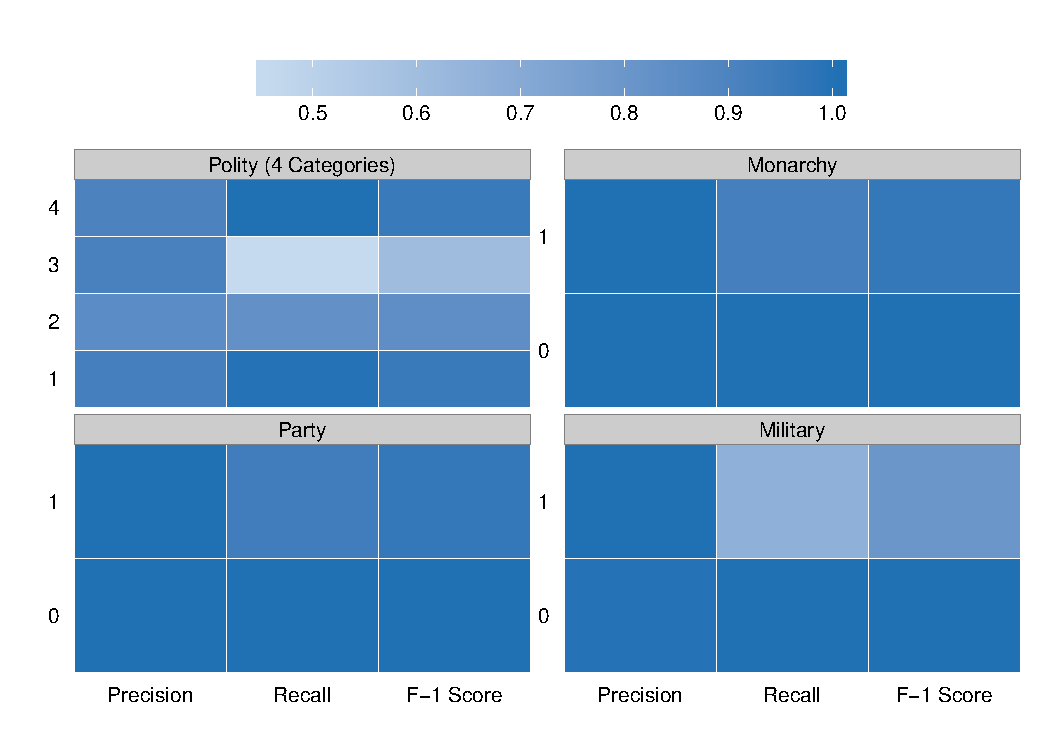
\includegraphics[width=.7\textwidth]{allClassPerf}		
\end{figure}
\FloatBarrier

\begin{figure}[ht]
	\centering
	\begin{tabular}{ll}
    \hspace{-7mm}	
    \subfloat[][Polity$=$ -10 -- -6]{
		\resizebox{0.5\textwidth}{!}{% Created by tikzDevice version 0.8.1 on 2015-01-12 19:17:59
% !TEX encoding = UTF-8 Unicode
% Calculated string width 0 times
}	
        \label{fig:sepp1}} &
	\subfloat[][-5 -- 0]{
		\resizebox{0.5\textwidth}{!}{% Created by tikzDevice version 0.8.1 on 2015-01-12 19:17:59
% !TEX encoding = UTF-8 Unicode
% Calculated string width 0 times
}	
        \label{fig:sepp2}} \\
	\hspace{-7mm}	
    \subfloat[][1 -- 5]{
		\resizebox{0.5\textwidth}{!}{% Created by tikzDevice version 0.8.1 on 2015-01-12 19:17:59
% !TEX encoding = UTF-8 Unicode
% Calculated string width 0 times
}	
        \label{fig:sepp3}} &
    \subfloat[][6 -- 10]{
		\resizebox{0.5\textwidth}{!}{% Created by tikzDevice version 0.8.1 on 2015-01-12 19:17:59
% !TEX encoding = UTF-8 Unicode
% Calculated string width 0 times
}	
        \label{fig:sepp4}}
    \end{tabular}
    \caption{Separation Plots of Out-of-Sample Predictions from Support Vector Machines (SVM) of Polity}
\end{figure}
\FloatBarrier

\begin{figure}[ht]
	\centering
	\begin{tabular}{l}
    \hspace{-7mm}	
    \subfloat[][Military]{
		\resizebox{0.33\textwidth}{!}{% Created by tikzDevice version 0.8.1 on 2015-01-12 19:17:59
% !TEX encoding = UTF-8 Unicode
% Calculated string width 0 times
}	
        \label{fig:sepmil}} &
    \subfloat[][Monarchy]{
		\resizebox{0.33\textwidth}{!}{% Created by tikzDevice version 0.8.1 on 2015-01-12 19:17:59
% !TEX encoding = UTF-8 Unicode
% Calculated string width 0 times
}	
        \label{fig:sepmon}} &
    \subfloat[][Party]{
		\resizebox{0.33\textwidth}{!}{% Created by tikzDevice version 0.8.1 on 2015-01-12 19:17:59
% !TEX encoding = UTF-8 Unicode
% Calculated string width 0 times
}	
        \label{fig:sepparty}}
    \end{tabular}
    \caption{Separation Plots of Out-of-Sample Predictions from Support Vector Machines (SVM) of Polity}
\end{figure}
\FloatBarrier

** Then go into features that predict classes again using word clouds

\begin{figure}[ht]
	\centering
	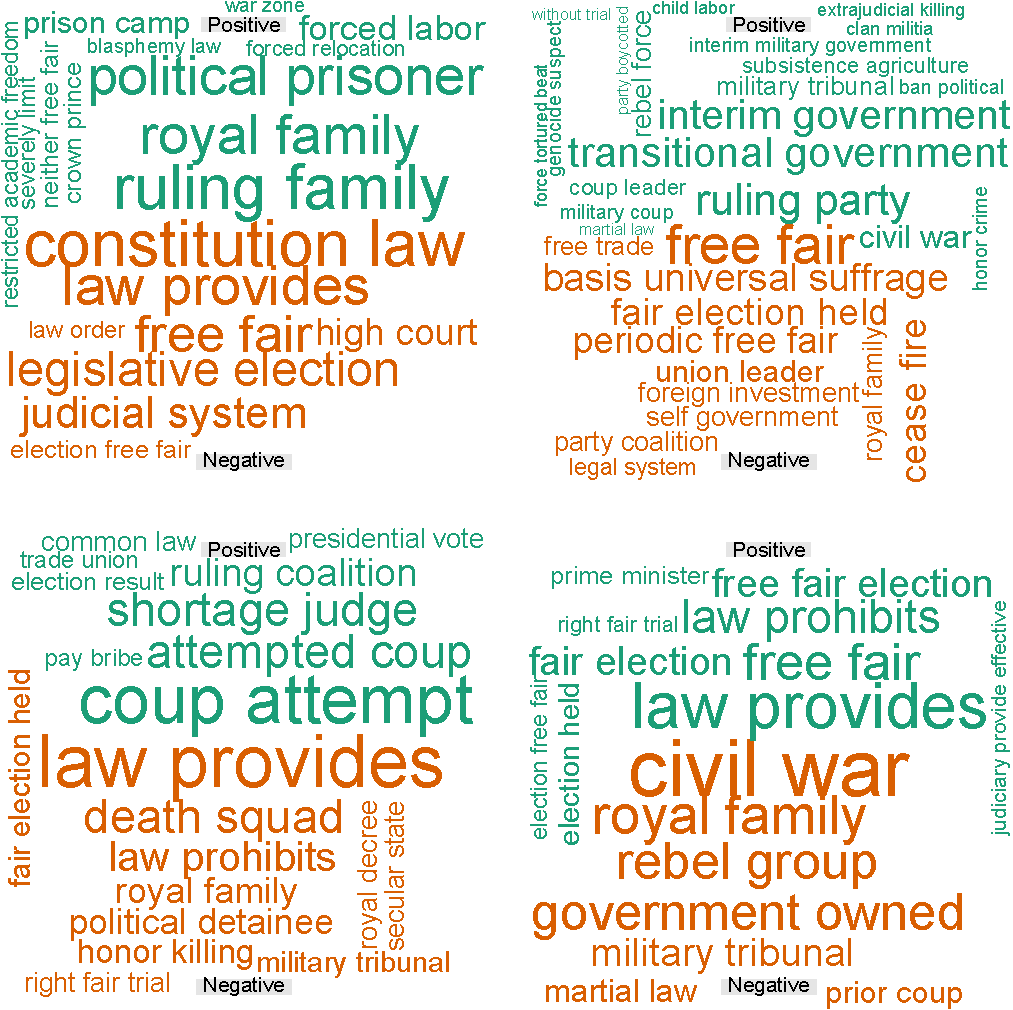
\includegraphics[width=.7\textwidth]{polCat_wrdCloud}
\end{figure}
\FloatBarrier

\begin{figure}[ht]
	\centering
	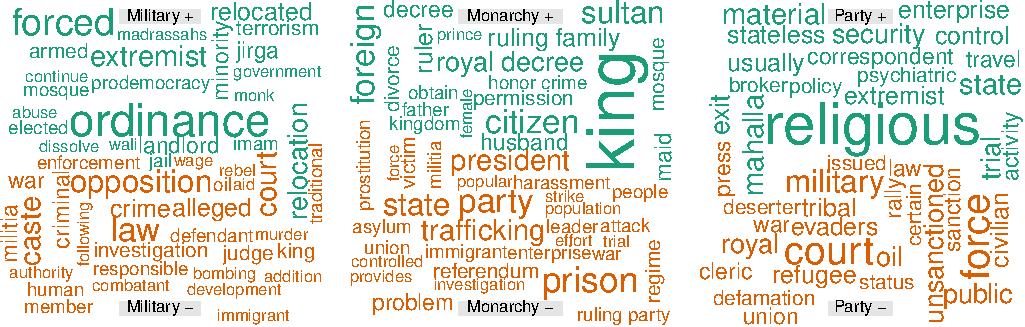
\includegraphics[width=.7\textwidth]{bin_wrdCloud}
\end{figure}
\FloatBarrier

** Discussion of what we are actually capturing here....

** Provide maps to give some context of how we are classifying countries and keep Jay's comments about it in there

The histograms in Figures 1A and 1B, on the following two pages, summarize the distribution of the out-of-sample predicted probabilities from SVM and logistic regression, respectively, for each of the four regime types we have explored so far.  The plots for the SVM estimates show sharp differentiation among cases, especially for the three authoritarian dimensions. Nearly all cases score very close to 0 or 1, producing bimodal distributions with steep peaks and few observations in between them. By contrast, the plots for the predicted probabilities from logistic regression are all unimodal, with a peak close to 0, maximum values much lower than 1, and thicker tails than the SVM output. 

If we compare these predicted probabilities to the observed values in the test set, we see that these classifiers are doing a very good job discriminating between 1s and 0s on the observed values for all four of the regime types. The column chart in Figure 2 summarizes the out-of-sample accuracy of SVM and logistic regression for each of the four types. SVM consistently outperforms logistic regression and produces extremely good results overall, albeit with some variation across the four types. For the three authoritarian types, precision (the proportion of cases classified as positive that actually belong there) was better than recall (the proportion of positive cases that were correctly classified), but that pattern is reversed for democracy. Logistic regression does noticeably poorer for all four types than SVM, but still not terribly.

\begin{figure}[ht]
	\centering
	\resizebox{0.7\textwidth}{!}{% Created by tikzDevice version 0.8.1 on 2015-01-12 17:01:40
% !TEX encoding = UTF-8 Unicode
% Calculated string width of 0.00 as 17.062600
% Calculated character metrics. ascent: 6.611760, descent: 0.000000, width: 8.797910
% Calculated string width of 0.05 as 17.062600
% Calculated string width of 0.10 as 17.062600
% Calculated string width of 0.15 as 17.062600
% Calculated string width of 0.20 as 17.062600
% Calculated string width of 0.00 as 17.062600
% Calculated string width of 0.05 as 17.062600
% Calculated string width of 0.10 as 17.062600
% Calculated string width of 0.15 as 17.062600
% Calculated string width of 0.20 as 17.062600
% Calculated string width of -10 to -6 as 35.724850
% Calculated string width of -5 to 0 as 27.726750
% Calculated string width of 1 to 5 as 24.527510
% Calculated string width of 6 to 10 as 29.326370
% Calculated string width of 0.00 as 17.062600
% Calculated string width of 0.25 as 17.062600
% Calculated string width of 0.50 as 17.062600
% Calculated string width of 0.75 as 17.062600
% Calculated string width of 1.00 as 17.062600
% Calculated string width of 0.00 as 17.062600
% Calculated string width of 0.25 as 17.062600
% Calculated string width of 0.50 as 17.062600
% Calculated string width of 0.75 as 17.062600
% Calculated string width of 1.00 as 17.062600
% Calculated string width of Proportion as 57.219210
% Calculated character metrics. ascent: 8.264620, descent: 0.000000, width: 10.997280
% Calculated string width of Estimated Probability as 116.404600
% Calculated string width of Proportion as 57.219210
% Calculated string width of Estimated Probability as 116.404600
% Drawing Rectangle from x0 = 0.000000, y0 = 0.000000 to x1 = 505.890000, y1 = 361.350000
% Beginning new tikzpicture 'page'
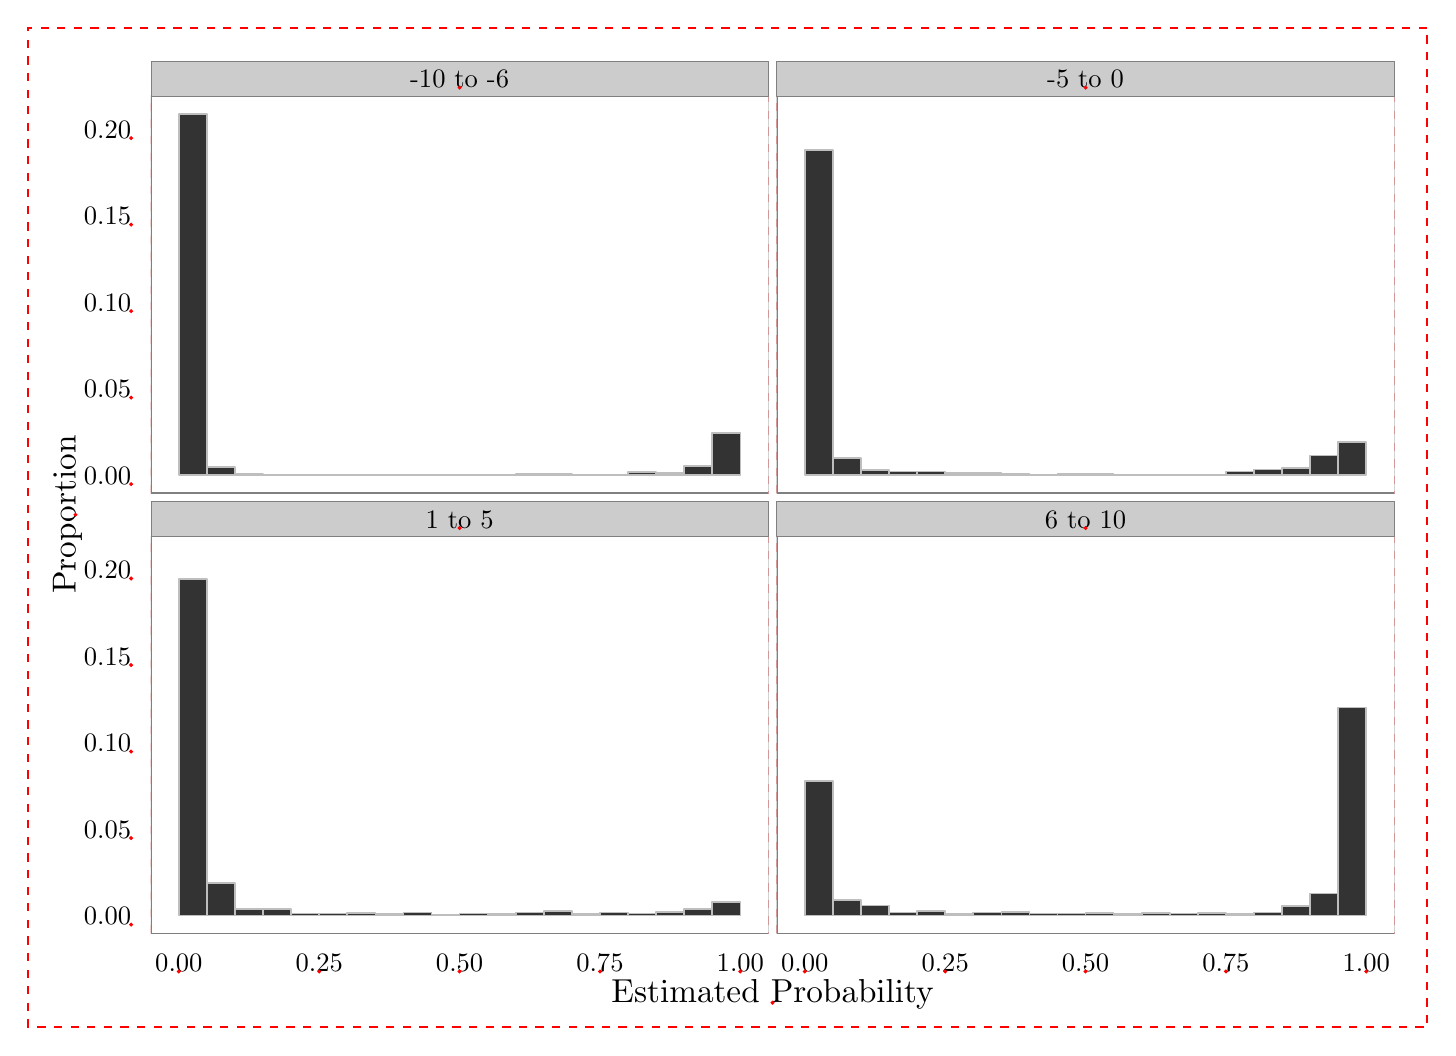
\begin{tikzpicture}[x=1pt,y=1pt]
\definecolor{fillColor}{RGB}{255,255,255}
\path[use as bounding box,fill=fillColor,fill opacity=0.00] (0,0) rectangle (505.89,361.35);
\begin{scope}
\path[clip] (  0.00,  0.00) rectangle (505.89,361.35);
\path[draw=red,very thick,dashed] (  0.00,  0.00) rectangle (505.89,361.35);
\definecolor{drawColor}{RGB}{255,255,255}
\definecolor{fillColor}{RGB}{255,255,255}

\path[draw=drawColor,line width= 0.6pt,line join=round,line cap=round,fill=fillColor] (  0.00,  0.00) rectangle (505.89,361.35);
\end{scope}
% Drawing Rectangle from x0 = 44.485409, y0 = 193.175409 to x1 = 267.659579, y1 = 336.670740
\begin{scope}
\path[clip] ( 44.49,193.18) rectangle (267.66,336.67);
\path[draw=red,very thick,dashed] ( 44.49,193.18) rectangle (267.66,336.67);
\definecolor{fillColor}{RGB}{255,255,255}

\path[fill=fillColor] ( 44.49,193.18) rectangle (267.66,336.67);
% Drawing Rectangle from x0 = 54.629689, y0 = 199.697925 to x1 = 64.773970, y1 = 330.148225
\definecolor{drawColor}{RGB}{190,190,190}
\definecolor{fillColor}{gray}{0.20}

\path[draw=drawColor,line width= 0.6pt,line join=round,fill=fillColor] ( 54.63,199.70) rectangle ( 64.77,330.15);
% Drawing Rectangle from x0 = 64.773970, y0 = 199.697925 to x1 = 74.918250, y1 = 202.572253

\path[draw=drawColor,line width= 0.6pt,line join=round,fill=fillColor] ( 64.77,199.70) rectangle ( 74.92,202.57);
% Drawing Rectangle from x0 = 74.918250, y0 = 199.697925 to x1 = 85.062531, y1 = 200.140129

\path[draw=drawColor,line width= 0.6pt,line join=round,fill=fillColor] ( 74.92,199.70) rectangle ( 85.06,200.14);
% Drawing Rectangle from x0 = 85.062531, y0 = 199.697925 to x1 = 95.206811, y1 = 199.919027

\path[draw=drawColor,line width= 0.6pt,line join=round,fill=fillColor] ( 85.06,199.70) rectangle ( 95.21,199.92);
% Drawing Rectangle from x0 = 95.206811, y0 = 199.697925 to x1 = 105.351092, y1 = 199.697925

\path[draw=drawColor,line width= 0.6pt,line join=round,fill=fillColor] ( 95.21,199.70) rectangle (105.35,199.70);
% Drawing Rectangle from x0 = 105.351092, y0 = 199.697925 to x1 = 115.495372, y1 = 199.697925

\path[draw=drawColor,line width= 0.6pt,line join=round,fill=fillColor] (105.35,199.70) rectangle (115.50,199.70);
% Drawing Rectangle from x0 = 115.495372, y0 = 199.697925 to x1 = 125.639653, y1 = 199.919027

\path[draw=drawColor,line width= 0.6pt,line join=round,fill=fillColor] (115.50,199.70) rectangle (125.64,199.92);
% Drawing Rectangle from x0 = 125.639653, y0 = 199.697925 to x1 = 135.783933, y1 = 199.919027

\path[draw=drawColor,line width= 0.6pt,line join=round,fill=fillColor] (125.64,199.70) rectangle (135.78,199.92);
% Drawing Rectangle from x0 = 135.783933, y0 = 199.697925 to x1 = 145.928214, y1 = 199.919027

\path[draw=drawColor,line width= 0.6pt,line join=round,fill=fillColor] (135.78,199.70) rectangle (145.93,199.92);
% Drawing Rectangle from x0 = 145.928214, y0 = 199.697925 to x1 = 156.072494, y1 = 199.919027

\path[draw=drawColor,line width= 0.6pt,line join=round,fill=fillColor] (145.93,199.70) rectangle (156.07,199.92);
% Drawing Rectangle from x0 = 156.072494, y0 = 199.697925 to x1 = 166.216775, y1 = 199.697925

\path[draw=drawColor,line width= 0.6pt,line join=round,fill=fillColor] (156.07,199.70) rectangle (166.22,199.70);
% Drawing Rectangle from x0 = 166.216775, y0 = 199.697925 to x1 = 176.361055, y1 = 199.697925

\path[draw=drawColor,line width= 0.6pt,line join=round,fill=fillColor] (166.22,199.70) rectangle (176.36,199.70);
% Drawing Rectangle from x0 = 176.361055, y0 = 199.697925 to x1 = 186.505336, y1 = 200.140129

\path[draw=drawColor,line width= 0.6pt,line join=round,fill=fillColor] (176.36,199.70) rectangle (186.51,200.14);
% Drawing Rectangle from x0 = 186.505336, y0 = 199.697925 to x1 = 196.649616, y1 = 200.140129

\path[draw=drawColor,line width= 0.6pt,line join=round,fill=fillColor] (186.51,199.70) rectangle (196.65,200.14);
% Drawing Rectangle from x0 = 196.649616, y0 = 199.697925 to x1 = 206.793897, y1 = 199.697925

\path[draw=drawColor,line width= 0.6pt,line join=round,fill=fillColor] (196.65,199.70) rectangle (206.79,199.70);
% Drawing Rectangle from x0 = 206.793897, y0 = 199.697925 to x1 = 216.938177, y1 = 199.919027

\path[draw=drawColor,line width= 0.6pt,line join=round,fill=fillColor] (206.79,199.70) rectangle (216.94,199.92);
% Drawing Rectangle from x0 = 216.938177, y0 = 199.697925 to x1 = 227.082458, y1 = 200.803436

\path[draw=drawColor,line width= 0.6pt,line join=round,fill=fillColor] (216.94,199.70) rectangle (227.08,200.80);
% Drawing Rectangle from x0 = 227.082458, y0 = 199.697925 to x1 = 237.226738, y1 = 200.361231

\path[draw=drawColor,line width= 0.6pt,line join=round,fill=fillColor] (227.08,199.70) rectangle (237.23,200.36);
% Drawing Rectangle from x0 = 237.226738, y0 = 199.697925 to x1 = 247.371019, y1 = 203.014458

\path[draw=drawColor,line width= 0.6pt,line join=round,fill=fillColor] (237.23,199.70) rectangle (247.37,203.01);
% Drawing Rectangle from x0 = 247.371019, y0 = 199.697925 to x1 = 257.515299, y1 = 214.953977

\path[draw=drawColor,line width= 0.6pt,line join=round,fill=fillColor] (247.37,199.70) rectangle (257.52,214.95);
% Drawing Rectangle from x0 = 44.485409, y0 = 193.175409 to x1 = 267.659579, y1 = 336.670740
\definecolor{drawColor}{gray}{0.50}

\path[draw=drawColor,line width= 0.6pt,line join=round,line cap=round] ( 44.49,193.18) rectangle (267.66,336.67);
\end{scope}
% Drawing Rectangle from x0 = 270.670829, y0 = 193.175409 to x1 = 493.845000, y1 = 336.670740
\begin{scope}
\path[clip] (270.67,193.18) rectangle (493.85,336.67);
\path[draw=red,very thick,dashed] (270.67,193.18) rectangle (493.85,336.67);
\definecolor{fillColor}{RGB}{255,255,255}

\path[fill=fillColor] (270.67,193.18) rectangle (493.85,336.67);
% Drawing Rectangle from x0 = 280.815110, y0 = 199.697925 to x1 = 290.959390, y1 = 317.103195
\definecolor{drawColor}{RGB}{190,190,190}
\definecolor{fillColor}{gray}{0.20}

\path[draw=drawColor,line width= 0.6pt,line join=round,fill=fillColor] (280.82,199.70) rectangle (290.96,317.10);
% Drawing Rectangle from x0 = 290.959390, y0 = 199.697925 to x1 = 301.103671, y1 = 205.888786

\path[draw=drawColor,line width= 0.6pt,line join=round,fill=fillColor] (290.96,199.70) rectangle (301.10,205.89);
% Drawing Rectangle from x0 = 301.103671, y0 = 199.697925 to x1 = 311.247951, y1 = 201.466742

\path[draw=drawColor,line width= 0.6pt,line join=round,fill=fillColor] (301.10,199.70) rectangle (311.25,201.47);
% Drawing Rectangle from x0 = 311.247951, y0 = 199.697925 to x1 = 321.392232, y1 = 201.024538

\path[draw=drawColor,line width= 0.6pt,line join=round,fill=fillColor] (311.25,199.70) rectangle (321.39,201.02);
% Drawing Rectangle from x0 = 321.392232, y0 = 199.697925 to x1 = 331.536512, y1 = 201.024538

\path[draw=drawColor,line width= 0.6pt,line join=round,fill=fillColor] (321.39,199.70) rectangle (331.54,201.02);
% Drawing Rectangle from x0 = 331.536512, y0 = 199.697925 to x1 = 341.680793, y1 = 200.361231

\path[draw=drawColor,line width= 0.6pt,line join=round,fill=fillColor] (331.54,199.70) rectangle (341.68,200.36);
% Drawing Rectangle from x0 = 341.680793, y0 = 199.697925 to x1 = 351.825073, y1 = 200.361231

\path[draw=drawColor,line width= 0.6pt,line join=round,fill=fillColor] (341.68,199.70) rectangle (351.83,200.36);
% Drawing Rectangle from x0 = 351.825073, y0 = 199.697925 to x1 = 361.969354, y1 = 200.140129

\path[draw=drawColor,line width= 0.6pt,line join=round,fill=fillColor] (351.83,199.70) rectangle (361.97,200.14);
% Drawing Rectangle from x0 = 361.969354, y0 = 199.697925 to x1 = 372.113634, y1 = 199.919027

\path[draw=drawColor,line width= 0.6pt,line join=round,fill=fillColor] (361.97,199.70) rectangle (372.11,199.92);
% Drawing Rectangle from x0 = 372.113634, y0 = 199.697925 to x1 = 382.257915, y1 = 200.140129

\path[draw=drawColor,line width= 0.6pt,line join=round,fill=fillColor] (372.11,199.70) rectangle (382.26,200.14);
% Drawing Rectangle from x0 = 382.257915, y0 = 199.697925 to x1 = 392.402195, y1 = 200.140129

\path[draw=drawColor,line width= 0.6pt,line join=round,fill=fillColor] (382.26,199.70) rectangle (392.40,200.14);
% Drawing Rectangle from x0 = 392.402195, y0 = 199.697925 to x1 = 402.546476, y1 = 199.919027

\path[draw=drawColor,line width= 0.6pt,line join=round,fill=fillColor] (392.40,199.70) rectangle (402.55,199.92);
% Drawing Rectangle from x0 = 402.546476, y0 = 199.697925 to x1 = 412.690756, y1 = 199.919027

\path[draw=drawColor,line width= 0.6pt,line join=round,fill=fillColor] (402.55,199.70) rectangle (412.69,199.92);
% Drawing Rectangle from x0 = 412.690756, y0 = 199.697925 to x1 = 422.835037, y1 = 199.697925

\path[draw=drawColor,line width= 0.6pt,line join=round,fill=fillColor] (412.69,199.70) rectangle (422.84,199.70);
% Drawing Rectangle from x0 = 422.835037, y0 = 199.697925 to x1 = 432.979317, y1 = 199.919027

\path[draw=drawColor,line width= 0.6pt,line join=round,fill=fillColor] (422.84,199.70) rectangle (432.98,199.92);
% Drawing Rectangle from x0 = 432.979317, y0 = 199.697925 to x1 = 443.123598, y1 = 201.024538

\path[draw=drawColor,line width= 0.6pt,line join=round,fill=fillColor] (432.98,199.70) rectangle (443.12,201.02);
% Drawing Rectangle from x0 = 443.123598, y0 = 199.697925 to x1 = 453.267878, y1 = 201.687844

\path[draw=drawColor,line width= 0.6pt,line join=round,fill=fillColor] (443.12,199.70) rectangle (453.27,201.69);
% Drawing Rectangle from x0 = 453.267878, y0 = 199.697925 to x1 = 463.412159, y1 = 202.130049

\path[draw=drawColor,line width= 0.6pt,line join=round,fill=fillColor] (453.27,199.70) rectangle (463.41,202.13);
% Drawing Rectangle from x0 = 463.412159, y0 = 199.697925 to x1 = 473.556439, y1 = 206.773195

\path[draw=drawColor,line width= 0.6pt,line join=round,fill=fillColor] (463.41,199.70) rectangle (473.56,206.77);
% Drawing Rectangle from x0 = 473.556439, y0 = 199.697925 to x1 = 483.700720, y1 = 211.637444

\path[draw=drawColor,line width= 0.6pt,line join=round,fill=fillColor] (473.56,199.70) rectangle (483.70,211.64);
% Drawing Rectangle from x0 = 270.670829, y0 = 193.175409 to x1 = 493.845000, y1 = 336.670740
\definecolor{drawColor}{gray}{0.50}

\path[draw=drawColor,line width= 0.6pt,line join=round,line cap=round] (270.67,193.18) rectangle (493.85,336.67);
\end{scope}
% Drawing Rectangle from x0 = 44.485409, y0 = 34.034569 to x1 = 267.659579, y1 = 177.529899
\begin{scope}
\path[clip] ( 44.49, 34.03) rectangle (267.66,177.53);
\path[draw=red,very thick,dashed] ( 44.49, 34.03) rectangle (267.66,177.53);
\definecolor{fillColor}{RGB}{255,255,255}

\path[fill=fillColor] ( 44.49, 34.03) rectangle (267.66,177.53);
% Drawing Rectangle from x0 = 54.629689, y0 = 40.557084 to x1 = 64.773970, y1 = 162.163296
\definecolor{drawColor}{RGB}{190,190,190}
\definecolor{fillColor}{gray}{0.20}

\path[draw=drawColor,line width= 0.6pt,line join=round,fill=fillColor] ( 54.63, 40.56) rectangle ( 64.77,162.16);
% Drawing Rectangle from x0 = 64.773970, y0 = 40.557084 to x1 = 74.918250, y1 = 52.275501

\path[draw=drawColor,line width= 0.6pt,line join=round,fill=fillColor] ( 64.77, 40.56) rectangle ( 74.92, 52.28);
% Drawing Rectangle from x0 = 74.918250, y0 = 40.557084 to x1 = 85.062531, y1 = 42.989208

\path[draw=drawColor,line width= 0.6pt,line join=round,fill=fillColor] ( 74.92, 40.56) rectangle ( 85.06, 42.99);
% Drawing Rectangle from x0 = 85.062531, y0 = 40.557084 to x1 = 95.206811, y1 = 42.768106

\path[draw=drawColor,line width= 0.6pt,line join=round,fill=fillColor] ( 85.06, 40.56) rectangle ( 95.21, 42.77);
% Drawing Rectangle from x0 = 95.206811, y0 = 40.557084 to x1 = 105.351092, y1 = 41.220391

\path[draw=drawColor,line width= 0.6pt,line join=round,fill=fillColor] ( 95.21, 40.56) rectangle (105.35, 41.22);
% Drawing Rectangle from x0 = 105.351092, y0 = 40.557084 to x1 = 115.495372, y1 = 41.220391

\path[draw=drawColor,line width= 0.6pt,line join=round,fill=fillColor] (105.35, 40.56) rectangle (115.50, 41.22);
% Drawing Rectangle from x0 = 115.495372, y0 = 40.557084 to x1 = 125.639653, y1 = 41.441493

\path[draw=drawColor,line width= 0.6pt,line join=round,fill=fillColor] (115.50, 40.56) rectangle (125.64, 41.44);
% Drawing Rectangle from x0 = 125.639653, y0 = 40.557084 to x1 = 135.783933, y1 = 40.999288

\path[draw=drawColor,line width= 0.6pt,line join=round,fill=fillColor] (125.64, 40.56) rectangle (135.78, 41.00);
% Drawing Rectangle from x0 = 135.783933, y0 = 40.557084 to x1 = 145.928214, y1 = 41.662595

\path[draw=drawColor,line width= 0.6pt,line join=round,fill=fillColor] (135.78, 40.56) rectangle (145.93, 41.66);
% Drawing Rectangle from x0 = 145.928214, y0 = 40.557084 to x1 = 156.072494, y1 = 40.778186

\path[draw=drawColor,line width= 0.6pt,line join=round,fill=fillColor] (145.93, 40.56) rectangle (156.07, 40.78);
% Drawing Rectangle from x0 = 156.072494, y0 = 40.557084 to x1 = 166.216775, y1 = 41.220391

\path[draw=drawColor,line width= 0.6pt,line join=round,fill=fillColor] (156.07, 40.56) rectangle (166.22, 41.22);
% Drawing Rectangle from x0 = 166.216775, y0 = 40.557084 to x1 = 176.361055, y1 = 40.999288

\path[draw=drawColor,line width= 0.6pt,line join=round,fill=fillColor] (166.22, 40.56) rectangle (176.36, 41.00);
% Drawing Rectangle from x0 = 176.361055, y0 = 40.557084 to x1 = 186.505336, y1 = 41.662595

\path[draw=drawColor,line width= 0.6pt,line join=round,fill=fillColor] (176.36, 40.56) rectangle (186.51, 41.66);
% Drawing Rectangle from x0 = 186.505336, y0 = 40.557084 to x1 = 196.649616, y1 = 42.104799

\path[draw=drawColor,line width= 0.6pt,line join=round,fill=fillColor] (186.51, 40.56) rectangle (196.65, 42.10);
% Drawing Rectangle from x0 = 196.649616, y0 = 40.557084 to x1 = 206.793897, y1 = 40.999288

\path[draw=drawColor,line width= 0.6pt,line join=round,fill=fillColor] (196.65, 40.56) rectangle (206.79, 41.00);
% Drawing Rectangle from x0 = 206.793897, y0 = 40.557084 to x1 = 216.938177, y1 = 41.662595

\path[draw=drawColor,line width= 0.6pt,line join=round,fill=fillColor] (206.79, 40.56) rectangle (216.94, 41.66);
% Drawing Rectangle from x0 = 216.938177, y0 = 40.557084 to x1 = 227.082458, y1 = 41.220391

\path[draw=drawColor,line width= 0.6pt,line join=round,fill=fillColor] (216.94, 40.56) rectangle (227.08, 41.22);
% Drawing Rectangle from x0 = 227.082458, y0 = 40.557084 to x1 = 237.226738, y1 = 41.883697

\path[draw=drawColor,line width= 0.6pt,line join=round,fill=fillColor] (227.08, 40.56) rectangle (237.23, 41.88);
% Drawing Rectangle from x0 = 237.226738, y0 = 40.557084 to x1 = 247.371019, y1 = 42.768106

\path[draw=drawColor,line width= 0.6pt,line join=round,fill=fillColor] (237.23, 40.56) rectangle (247.37, 42.77);
% Drawing Rectangle from x0 = 247.371019, y0 = 40.557084 to x1 = 257.515299, y1 = 45.421332

\path[draw=drawColor,line width= 0.6pt,line join=round,fill=fillColor] (247.37, 40.56) rectangle (257.52, 45.42);
% Drawing Rectangle from x0 = 44.485409, y0 = 34.034569 to x1 = 267.659579, y1 = 177.529899
\definecolor{drawColor}{gray}{0.50}

\path[draw=drawColor,line width= 0.6pt,line join=round,line cap=round] ( 44.49, 34.03) rectangle (267.66,177.53);
\end{scope}
% Drawing Rectangle from x0 = 270.670829, y0 = 34.034569 to x1 = 493.845000, y1 = 177.529899
\begin{scope}
\path[clip] (270.67, 34.03) rectangle (493.85,177.53);
\path[draw=red,very thick,dashed] (270.67, 34.03) rectangle (493.85,177.53);
\definecolor{fillColor}{RGB}{255,255,255}

\path[fill=fillColor] (270.67, 34.03) rectangle (493.85,177.53);
% Drawing Rectangle from x0 = 280.815110, y0 = 40.557084 to x1 = 290.959390, y1 = 89.199569
\definecolor{drawColor}{RGB}{190,190,190}
\definecolor{fillColor}{gray}{0.20}

\path[draw=drawColor,line width= 0.6pt,line join=round,fill=fillColor] (280.82, 40.56) rectangle (290.96, 89.20);
% Drawing Rectangle from x0 = 290.959390, y0 = 40.557084 to x1 = 301.103671, y1 = 46.084639

\path[draw=drawColor,line width= 0.6pt,line join=round,fill=fillColor] (290.96, 40.56) rectangle (301.10, 46.08);
% Drawing Rectangle from x0 = 301.103671, y0 = 40.557084 to x1 = 311.247951, y1 = 44.094719

\path[draw=drawColor,line width= 0.6pt,line join=round,fill=fillColor] (301.10, 40.56) rectangle (311.25, 44.09);
% Drawing Rectangle from x0 = 311.247951, y0 = 40.557084 to x1 = 321.392232, y1 = 41.662595

\path[draw=drawColor,line width= 0.6pt,line join=round,fill=fillColor] (311.25, 40.56) rectangle (321.39, 41.66);
% Drawing Rectangle from x0 = 321.392232, y0 = 40.557084 to x1 = 331.536512, y1 = 42.104799

\path[draw=drawColor,line width= 0.6pt,line join=round,fill=fillColor] (321.39, 40.56) rectangle (331.54, 42.10);
% Drawing Rectangle from x0 = 331.536512, y0 = 40.557084 to x1 = 341.680793, y1 = 40.999288

\path[draw=drawColor,line width= 0.6pt,line join=round,fill=fillColor] (331.54, 40.56) rectangle (341.68, 41.00);
% Drawing Rectangle from x0 = 341.680793, y0 = 40.557084 to x1 = 351.825073, y1 = 41.662595

\path[draw=drawColor,line width= 0.6pt,line join=round,fill=fillColor] (341.68, 40.56) rectangle (351.83, 41.66);
% Drawing Rectangle from x0 = 351.825073, y0 = 40.557084 to x1 = 361.969354, y1 = 41.883697

\path[draw=drawColor,line width= 0.6pt,line join=round,fill=fillColor] (351.83, 40.56) rectangle (361.97, 41.88);
% Drawing Rectangle from x0 = 361.969354, y0 = 40.557084 to x1 = 372.113634, y1 = 41.220391

\path[draw=drawColor,line width= 0.6pt,line join=round,fill=fillColor] (361.97, 40.56) rectangle (372.11, 41.22);
% Drawing Rectangle from x0 = 372.113634, y0 = 40.557084 to x1 = 382.257915, y1 = 41.220391

\path[draw=drawColor,line width= 0.6pt,line join=round,fill=fillColor] (372.11, 40.56) rectangle (382.26, 41.22);
% Drawing Rectangle from x0 = 382.257915, y0 = 40.557084 to x1 = 392.402195, y1 = 41.441493

\path[draw=drawColor,line width= 0.6pt,line join=round,fill=fillColor] (382.26, 40.56) rectangle (392.40, 41.44);
% Drawing Rectangle from x0 = 392.402195, y0 = 40.557084 to x1 = 402.546476, y1 = 40.999288

\path[draw=drawColor,line width= 0.6pt,line join=round,fill=fillColor] (392.40, 40.56) rectangle (402.55, 41.00);
% Drawing Rectangle from x0 = 402.546476, y0 = 40.557084 to x1 = 412.690756, y1 = 41.441493

\path[draw=drawColor,line width= 0.6pt,line join=round,fill=fillColor] (402.55, 40.56) rectangle (412.69, 41.44);
% Drawing Rectangle from x0 = 412.690756, y0 = 40.557084 to x1 = 422.835037, y1 = 41.220391

\path[draw=drawColor,line width= 0.6pt,line join=round,fill=fillColor] (412.69, 40.56) rectangle (422.84, 41.22);
% Drawing Rectangle from x0 = 422.835037, y0 = 40.557084 to x1 = 432.979317, y1 = 41.441493

\path[draw=drawColor,line width= 0.6pt,line join=round,fill=fillColor] (422.84, 40.56) rectangle (432.98, 41.44);
% Drawing Rectangle from x0 = 432.979317, y0 = 40.557084 to x1 = 443.123598, y1 = 40.999288

\path[draw=drawColor,line width= 0.6pt,line join=round,fill=fillColor] (432.98, 40.56) rectangle (443.12, 41.00);
% Drawing Rectangle from x0 = 443.123598, y0 = 40.557084 to x1 = 453.267878, y1 = 41.662595

\path[draw=drawColor,line width= 0.6pt,line join=round,fill=fillColor] (443.12, 40.56) rectangle (453.27, 41.66);
% Drawing Rectangle from x0 = 453.267878, y0 = 40.557084 to x1 = 463.412159, y1 = 43.873617

\path[draw=drawColor,line width= 0.6pt,line join=round,fill=fillColor] (453.27, 40.56) rectangle (463.41, 43.87);
% Drawing Rectangle from x0 = 463.412159, y0 = 40.557084 to x1 = 473.556439, y1 = 48.516763

\path[draw=drawColor,line width= 0.6pt,line join=round,fill=fillColor] (463.41, 40.56) rectangle (473.56, 48.52);
% Drawing Rectangle from x0 = 473.556439, y0 = 40.557084 to x1 = 483.700720, y1 = 115.731833

\path[draw=drawColor,line width= 0.6pt,line join=round,fill=fillColor] (473.56, 40.56) rectangle (483.70,115.73);
% Drawing Rectangle from x0 = 270.670829, y0 = 34.034569 to x1 = 493.845000, y1 = 177.529899
\definecolor{drawColor}{gray}{0.50}

\path[draw=drawColor,line width= 0.6pt,line join=round,line cap=round] (270.67, 34.03) rectangle (493.85,177.53);
\end{scope}
% Drawing Rectangle from x0 = 44.485409, y0 = 336.670740 to x1 = 267.659579, y1 = 349.305000
\begin{scope}
\path[clip] (  0.00,  0.00) rectangle (505.89,361.35);
\path[draw=red,very thick,dashed] (  0.00,  0.00) rectangle (505.89,361.35);
\definecolor{drawColor}{gray}{0.50}
\definecolor{fillColor}{gray}{0.80}

\path[draw=drawColor,line width= 0.2pt,line join=round,line cap=round,fill=fillColor] ( 44.49,336.67) rectangle (267.66,349.31);
% Calculated string width of -10 to -6 as 35.724850
% Calculated character metrics. ascent: 6.611760, descent: 0.000000, width: 8.797910
% Drawing node at x = 156.072494, y = 339.681990
\definecolor{drawColor}{RGB}{0,0,0}

\node[text=drawColor,anchor=base,inner sep=0pt, outer sep=0pt, scale=  0.96] at (156.07,339.68) {-10 to -6};

\draw[color=red, fill=red] (156.07,339.68) circle (0.5pt);
\end{scope}
% Drawing Rectangle from x0 = 270.670829, y0 = 336.670740 to x1 = 493.845000, y1 = 349.305000
\begin{scope}
\path[clip] (  0.00,  0.00) rectangle (505.89,361.35);
\path[draw=red,very thick,dashed] (  0.00,  0.00) rectangle (505.89,361.35);
\definecolor{drawColor}{gray}{0.50}
\definecolor{fillColor}{gray}{0.80}

\path[draw=drawColor,line width= 0.2pt,line join=round,line cap=round,fill=fillColor] (270.67,336.67) rectangle (493.85,349.31);
% Calculated string width of -5 to 0 as 27.726750
% Drawing node at x = 382.257915, y = 339.681990
\definecolor{drawColor}{RGB}{0,0,0}

\node[text=drawColor,anchor=base,inner sep=0pt, outer sep=0pt, scale=  0.96] at (382.26,339.68) {-5 to 0};

\draw[color=red, fill=red] (382.26,339.68) circle (0.5pt);
\end{scope}
% Drawing Rectangle from x0 = 44.485409, y0 = 177.529899 to x1 = 267.659579, y1 = 190.164159
\begin{scope}
\path[clip] (  0.00,  0.00) rectangle (505.89,361.35);
\path[draw=red,very thick,dashed] (  0.00,  0.00) rectangle (505.89,361.35);
\definecolor{drawColor}{gray}{0.50}
\definecolor{fillColor}{gray}{0.80}

\path[draw=drawColor,line width= 0.2pt,line join=round,line cap=round,fill=fillColor] ( 44.49,177.53) rectangle (267.66,190.16);
% Calculated string width of 1 to 5 as 24.527510
% Drawing node at x = 156.072494, y = 180.541149
\definecolor{drawColor}{RGB}{0,0,0}

\node[text=drawColor,anchor=base,inner sep=0pt, outer sep=0pt, scale=  0.96] at (156.07,180.54) {1 to 5};

\draw[color=red, fill=red] (156.07,180.54) circle (0.5pt);
\end{scope}
% Drawing Rectangle from x0 = 270.670829, y0 = 177.529899 to x1 = 493.845000, y1 = 190.164159
\begin{scope}
\path[clip] (  0.00,  0.00) rectangle (505.89,361.35);
\path[draw=red,very thick,dashed] (  0.00,  0.00) rectangle (505.89,361.35);
\definecolor{drawColor}{gray}{0.50}
\definecolor{fillColor}{gray}{0.80}

\path[draw=drawColor,line width= 0.2pt,line join=round,line cap=round,fill=fillColor] (270.67,177.53) rectangle (493.85,190.16);
% Calculated string width of 6 to 10 as 29.326370
% Drawing node at x = 382.257915, y = 180.541149
\definecolor{drawColor}{RGB}{0,0,0}

\node[text=drawColor,anchor=base,inner sep=0pt, outer sep=0pt, scale=  0.96] at (382.26,180.54) {6 to 10};

\draw[color=red, fill=red] (382.26,180.54) circle (0.5pt);
\end{scope}
% Calculated string width of 0.00 as 17.062600
% Calculated string width of 0.05 as 17.062600
% Calculated string width of 0.10 as 17.062600
% Calculated string width of 0.15 as 17.062600
% Calculated string width of 0.20 as 17.062600
% Calculated string width of 0.00 as 17.062600
% Calculated string width of 0.05 as 17.062600
% Calculated string width of 0.10 as 17.062600
% Calculated string width of 0.15 as 17.062600
% Calculated string width of 0.20 as 17.062600
% Calculated string width of 0.00 as 17.062600
% Calculated string width of 0.05 as 17.062600
% Calculated string width of 0.10 as 17.062600
% Calculated string width of 0.15 as 17.062600
% Calculated string width of 0.20 as 17.062600
% Calculated string width of 0.00 as 17.062600
% Drawing node at x = 37.372220, y = 196.392045
\begin{scope}
\path[clip] (  0.00,  0.00) rectangle (505.89,361.35);
\path[draw=red,very thick,dashed] (  0.00,  0.00) rectangle (505.89,361.35);
\definecolor{drawColor}{RGB}{0,0,0}

\node[text=drawColor,anchor=base east,inner sep=0pt, outer sep=0pt, scale=  0.96] at ( 37.37,196.39) {0.00};

\draw[color=red, fill=red] ( 37.37,196.39) circle (0.5pt);
% Calculated string width of 0.05 as 17.062600
% Drawing node at x = 37.372220, y = 227.655896

\node[text=drawColor,anchor=base east,inner sep=0pt, outer sep=0pt, scale=  0.96] at ( 37.37,227.66) {0.05};

\draw[color=red, fill=red] ( 37.37,227.66) circle (0.5pt);
% Calculated string width of 0.10 as 17.062600
% Drawing node at x = 37.372220, y = 258.919748

\node[text=drawColor,anchor=base east,inner sep=0pt, outer sep=0pt, scale=  0.96] at ( 37.37,258.92) {0.10};

\draw[color=red, fill=red] ( 37.37,258.92) circle (0.5pt);
% Calculated string width of 0.15 as 17.062600
% Drawing node at x = 37.372220, y = 290.183600

\node[text=drawColor,anchor=base east,inner sep=0pt, outer sep=0pt, scale=  0.96] at ( 37.37,290.18) {0.15};

\draw[color=red, fill=red] ( 37.37,290.18) circle (0.5pt);
% Calculated string width of 0.20 as 17.062600
% Drawing node at x = 37.372220, y = 321.447451

\node[text=drawColor,anchor=base east,inner sep=0pt, outer sep=0pt, scale=  0.96] at ( 37.37,321.45) {0.20};

\draw[color=red, fill=red] ( 37.37,321.45) circle (0.5pt);
\end{scope}
% Calculated string width of 0.00 as 17.062600
% Calculated string width of 0.05 as 17.062600
% Calculated string width of 0.10 as 17.062600
% Calculated string width of 0.15 as 17.062600
% Calculated string width of 0.20 as 17.062600
% Calculated string width of 0.00 as 17.062600
% Calculated string width of 0.05 as 17.062600
% Calculated string width of 0.10 as 17.062600
% Calculated string width of 0.15 as 17.062600
% Calculated string width of 0.20 as 17.062600
% Calculated string width of 0.00 as 17.062600
% Calculated string width of 0.05 as 17.062600
% Calculated string width of 0.10 as 17.062600
% Calculated string width of 0.15 as 17.062600
% Calculated string width of 0.20 as 17.062600
% Calculated string width of 0.00 as 17.062600
% Drawing node at x = 37.372220, y = 37.251204
\begin{scope}
\path[clip] (  0.00,  0.00) rectangle (505.89,361.35);
\path[draw=red,very thick,dashed] (  0.00,  0.00) rectangle (505.89,361.35);
\definecolor{drawColor}{RGB}{0,0,0}

\node[text=drawColor,anchor=base east,inner sep=0pt, outer sep=0pt, scale=  0.96] at ( 37.37, 37.25) {0.00};

\draw[color=red, fill=red] ( 37.37, 37.25) circle (0.5pt);
% Calculated string width of 0.05 as 17.062600
% Drawing node at x = 37.372220, y = 68.515056

\node[text=drawColor,anchor=base east,inner sep=0pt, outer sep=0pt, scale=  0.96] at ( 37.37, 68.52) {0.05};

\draw[color=red, fill=red] ( 37.37, 68.52) circle (0.5pt);
% Calculated string width of 0.10 as 17.062600
% Drawing node at x = 37.372220, y = 99.778907

\node[text=drawColor,anchor=base east,inner sep=0pt, outer sep=0pt, scale=  0.96] at ( 37.37, 99.78) {0.10};

\draw[color=red, fill=red] ( 37.37, 99.78) circle (0.5pt);
% Calculated string width of 0.15 as 17.062600
% Drawing node at x = 37.372220, y = 131.042759

\node[text=drawColor,anchor=base east,inner sep=0pt, outer sep=0pt, scale=  0.96] at ( 37.37,131.04) {0.15};

\draw[color=red, fill=red] ( 37.37,131.04) circle (0.5pt);
% Calculated string width of 0.20 as 17.062600
% Drawing node at x = 37.372220, y = 162.306611

\node[text=drawColor,anchor=base east,inner sep=0pt, outer sep=0pt, scale=  0.96] at ( 37.37,162.31) {0.20};

\draw[color=red, fill=red] ( 37.37,162.31) circle (0.5pt);
\end{scope}
% Calculated string width of 0.00 as 17.062600
% Calculated string width of 0.25 as 17.062600
% Calculated string width of 0.50 as 17.062600
% Calculated string width of 0.75 as 17.062600
% Calculated string width of 1.00 as 17.062600
% Calculated string width of 0.00 as 17.062600
% Calculated string width of 0.25 as 17.062600
% Calculated string width of 0.50 as 17.062600
% Calculated string width of 0.75 as 17.062600
% Calculated string width of 1.00 as 17.062600
% Calculated string width of 0.00 as 17.062600
% Calculated string width of 0.25 as 17.062600
% Calculated string width of 0.50 as 17.062600
% Calculated string width of 0.75 as 17.062600
% Calculated string width of 1.00 as 17.062600
% Calculated string width of 0.00 as 17.062600
% Drawing node at x = 54.629689, y = 20.309620
\begin{scope}
\path[clip] (  0.00,  0.00) rectangle (505.89,361.35);
\path[draw=red,very thick,dashed] (  0.00,  0.00) rectangle (505.89,361.35);
\definecolor{drawColor}{RGB}{0,0,0}

\node[text=drawColor,anchor=base,inner sep=0pt, outer sep=0pt, scale=  0.96] at ( 54.63, 20.31) {0.00};

\draw[color=red, fill=red] ( 54.63, 20.31) circle (0.5pt);
% Calculated string width of 0.25 as 17.062600
% Drawing node at x = 105.351092, y = 20.309620

\node[text=drawColor,anchor=base,inner sep=0pt, outer sep=0pt, scale=  0.96] at (105.35, 20.31) {0.25};

\draw[color=red, fill=red] (105.35, 20.31) circle (0.5pt);
% Calculated string width of 0.50 as 17.062600
% Drawing node at x = 156.072494, y = 20.309620

\node[text=drawColor,anchor=base,inner sep=0pt, outer sep=0pt, scale=  0.96] at (156.07, 20.31) {0.50};

\draw[color=red, fill=red] (156.07, 20.31) circle (0.5pt);
% Calculated string width of 0.75 as 17.062600
% Drawing node at x = 206.793897, y = 20.309620

\node[text=drawColor,anchor=base,inner sep=0pt, outer sep=0pt, scale=  0.96] at (206.79, 20.31) {0.75};

\draw[color=red, fill=red] (206.79, 20.31) circle (0.5pt);
% Calculated string width of 1.00 as 17.062600
% Drawing node at x = 257.515299, y = 20.309620

\node[text=drawColor,anchor=base,inner sep=0pt, outer sep=0pt, scale=  0.96] at (257.52, 20.31) {1.00};

\draw[color=red, fill=red] (257.52, 20.31) circle (0.5pt);
\end{scope}
% Calculated string width of 0.00 as 17.062600
% Calculated string width of 0.25 as 17.062600
% Calculated string width of 0.50 as 17.062600
% Calculated string width of 0.75 as 17.062600
% Calculated string width of 1.00 as 17.062600
% Calculated string width of 0.00 as 17.062600
% Calculated string width of 0.25 as 17.062600
% Calculated string width of 0.50 as 17.062600
% Calculated string width of 0.75 as 17.062600
% Calculated string width of 1.00 as 17.062600
% Calculated string width of 0.00 as 17.062600
% Calculated string width of 0.25 as 17.062600
% Calculated string width of 0.50 as 17.062600
% Calculated string width of 0.75 as 17.062600
% Calculated string width of 1.00 as 17.062600
% Calculated string width of 0.00 as 17.062600
% Drawing node at x = 280.815110, y = 20.309620
\begin{scope}
\path[clip] (  0.00,  0.00) rectangle (505.89,361.35);
\path[draw=red,very thick,dashed] (  0.00,  0.00) rectangle (505.89,361.35);
\definecolor{drawColor}{RGB}{0,0,0}

\node[text=drawColor,anchor=base,inner sep=0pt, outer sep=0pt, scale=  0.96] at (280.82, 20.31) {0.00};

\draw[color=red, fill=red] (280.82, 20.31) circle (0.5pt);
% Calculated string width of 0.25 as 17.062600
% Drawing node at x = 331.536512, y = 20.309620

\node[text=drawColor,anchor=base,inner sep=0pt, outer sep=0pt, scale=  0.96] at (331.54, 20.31) {0.25};

\draw[color=red, fill=red] (331.54, 20.31) circle (0.5pt);
% Calculated string width of 0.50 as 17.062600
% Drawing node at x = 382.257915, y = 20.309620

\node[text=drawColor,anchor=base,inner sep=0pt, outer sep=0pt, scale=  0.96] at (382.26, 20.31) {0.50};

\draw[color=red, fill=red] (382.26, 20.31) circle (0.5pt);
% Calculated string width of 0.75 as 17.062600
% Drawing node at x = 432.979317, y = 20.309620

\node[text=drawColor,anchor=base,inner sep=0pt, outer sep=0pt, scale=  0.96] at (432.98, 20.31) {0.75};

\draw[color=red, fill=red] (432.98, 20.31) circle (0.5pt);
% Calculated string width of 1.00 as 17.062600
% Drawing node at x = 483.700720, y = 20.309620

\node[text=drawColor,anchor=base,inner sep=0pt, outer sep=0pt, scale=  0.96] at (483.70, 20.31) {1.00};

\draw[color=red, fill=red] (483.70, 20.31) circle (0.5pt);
\end{scope}
% Calculated string width of Estimated Probability as 116.404600
% Calculated character metrics. ascent: 8.264620, descent: 0.000000, width: 10.997280
% Drawing node at x = 269.165204, y = 9.033750
\begin{scope}
\path[clip] (  0.00,  0.00) rectangle (505.89,361.35);
\path[draw=red,very thick,dashed] (  0.00,  0.00) rectangle (505.89,361.35);
\definecolor{drawColor}{RGB}{0,0,0}

\node[text=drawColor,anchor=base,inner sep=0pt, outer sep=0pt, scale=  1.20] at (269.17,  9.03) {Estimated Probability};

\draw[color=red, fill=red] (269.17,  9.03) circle (0.5pt);
\end{scope}
% Calculated string width of Proportion as 57.219210
% Drawing node at x = 17.298370, y = 185.352654
\begin{scope}
\path[clip] (  0.00,  0.00) rectangle (505.89,361.35);
\path[draw=red,very thick,dashed] (  0.00,  0.00) rectangle (505.89,361.35);
\definecolor{drawColor}{RGB}{0,0,0}

\node[text=drawColor,rotate= 90.00,anchor=base,inner sep=0pt, outer sep=0pt, scale=  1.20] at ( 17.30,185.35) {Proportion};

\draw[color=red, fill=red] ( 17.30,185.35) circle (0.5pt);
\end{scope}
\end{tikzpicture}
% Calculated string width 114 times
}	
	\caption{Histograms of Out-of-Sample Estimated Probabilities of Four Regime Types from Support Vector Machines (SVM)}
\end{figure}

\begin{figure}[ht]
	\centering
	\resizebox{0.7\textwidth}{!}{% Created by tikzDevice version 0.7.0 on 2015-01-10 18:41:33
% !TEX encoding = UTF-8 Unicode
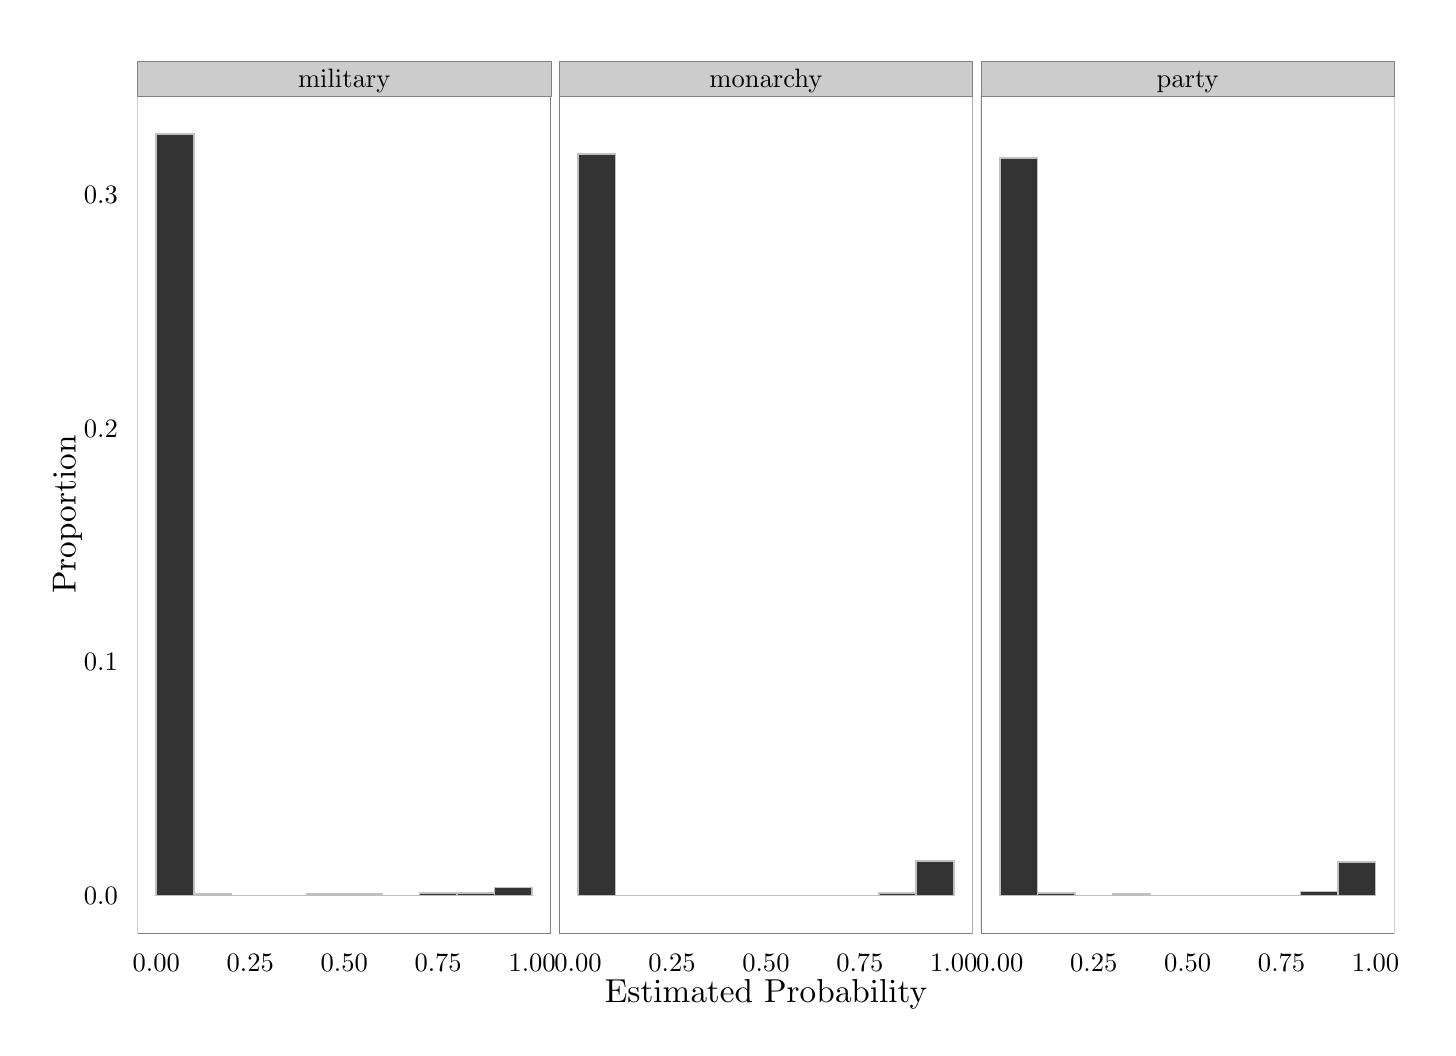
\begin{tikzpicture}[x=1pt,y=1pt]
\definecolor[named]{fillColor}{rgb}{1.00,1.00,1.00}
\path[use as bounding box,fill=fillColor,fill opacity=0.00] (0,0) rectangle (505.89,361.35);
\begin{scope}
\path[clip] (  0.00,  0.00) rectangle (505.89,361.35);
\definecolor[named]{drawColor}{rgb}{1.00,1.00,1.00}
\definecolor[named]{fillColor}{rgb}{1.00,1.00,1.00}

\path[draw=drawColor,line width= 0.6pt,line join=round,line cap=round,fill=fillColor] (  0.00,  0.00) rectangle (505.89,361.35);
\end{scope}
\begin{scope}
\path[clip] ( 39.69, 34.03) rectangle (189.07,336.67);
\definecolor[named]{fillColor}{rgb}{1.00,1.00,1.00}

\path[fill=fillColor] ( 39.69, 34.03) rectangle (189.07,336.67);
\definecolor[named]{drawColor}{rgb}{0.75,0.75,0.75}
\definecolor[named]{fillColor}{rgb}{0.20,0.20,0.20}

\path[draw=drawColor,line width= 0.6pt,line join=round,fill=fillColor] ( 46.48, 47.79) rectangle ( 60.06,322.91);

\path[draw=drawColor,line width= 0.6pt,line join=round,fill=fillColor] ( 60.06, 47.79) rectangle ( 73.64, 48.27);

\path[draw=drawColor,line width= 0.6pt,line join=round,fill=fillColor] ( 73.64, 47.79) rectangle ( 87.22, 47.79);

\path[draw=drawColor,line width= 0.6pt,line join=round,fill=fillColor] ( 87.22, 47.79) rectangle (100.80, 47.79);

\path[draw=drawColor,line width= 0.6pt,line join=round,fill=fillColor] (100.80, 47.79) rectangle (114.38, 48.27);

\path[draw=drawColor,line width= 0.6pt,line join=round,fill=fillColor] (114.38, 47.79) rectangle (127.96, 48.27);

\path[draw=drawColor,line width= 0.6pt,line join=round,fill=fillColor] (127.96, 47.79) rectangle (141.54, 47.79);

\path[draw=drawColor,line width= 0.6pt,line join=round,fill=fillColor] (141.54, 47.79) rectangle (155.12, 48.76);

\path[draw=drawColor,line width= 0.6pt,line join=round,fill=fillColor] (155.12, 47.79) rectangle (168.70, 48.76);

\path[draw=drawColor,line width= 0.6pt,line join=round,fill=fillColor] (168.70, 47.79) rectangle (182.28, 50.69);
\definecolor[named]{drawColor}{rgb}{0.50,0.50,0.50}

\path[draw=drawColor,line width= 0.6pt,line join=round,line cap=round] ( 39.69, 34.03) rectangle (189.07,336.67);
\end{scope}
\begin{scope}
\path[clip] (192.08, 34.03) rectangle (341.46,336.67);
\definecolor[named]{fillColor}{rgb}{1.00,1.00,1.00}

\path[fill=fillColor] (192.08, 34.03) rectangle (341.46,336.67);
\definecolor[named]{drawColor}{rgb}{0.75,0.75,0.75}
\definecolor[named]{fillColor}{rgb}{0.20,0.20,0.20}

\path[draw=drawColor,line width= 0.6pt,line join=round,fill=fillColor] (198.87, 47.79) rectangle (212.45,315.67);

\path[draw=drawColor,line width= 0.6pt,line join=round,fill=fillColor] (212.45, 47.79) rectangle (226.03, 47.79);

\path[draw=drawColor,line width= 0.6pt,line join=round,fill=fillColor] (226.03, 47.79) rectangle (239.61, 47.79);

\path[draw=drawColor,line width= 0.6pt,line join=round,fill=fillColor] (239.61, 47.79) rectangle (253.19, 47.79);

\path[draw=drawColor,line width= 0.6pt,line join=round,fill=fillColor] (253.19, 47.79) rectangle (266.77, 47.79);

\path[draw=drawColor,line width= 0.6pt,line join=round,fill=fillColor] (266.77, 47.79) rectangle (280.35, 47.79);

\path[draw=drawColor,line width= 0.6pt,line join=round,fill=fillColor] (280.35, 47.79) rectangle (293.93, 47.79);

\path[draw=drawColor,line width= 0.6pt,line join=round,fill=fillColor] (293.93, 47.79) rectangle (307.51, 47.79);

\path[draw=drawColor,line width= 0.6pt,line join=round,fill=fillColor] (307.51, 47.79) rectangle (321.09, 48.76);

\path[draw=drawColor,line width= 0.6pt,line join=round,fill=fillColor] (321.09, 47.79) rectangle (334.67, 60.34);
\definecolor[named]{drawColor}{rgb}{0.50,0.50,0.50}

\path[draw=drawColor,line width= 0.6pt,line join=round,line cap=round] (192.08, 34.03) rectangle (341.46,336.67);
\end{scope}
\begin{scope}
\path[clip] (344.47, 34.03) rectangle (493.85,336.67);
\definecolor[named]{fillColor}{rgb}{1.00,1.00,1.00}

\path[fill=fillColor] (344.47, 34.03) rectangle (493.85,336.67);
\definecolor[named]{drawColor}{rgb}{0.75,0.75,0.75}
\definecolor[named]{fillColor}{rgb}{0.20,0.20,0.20}

\path[draw=drawColor,line width= 0.6pt,line join=round,fill=fillColor] (351.26, 47.79) rectangle (364.84,314.23);

\path[draw=drawColor,line width= 0.6pt,line join=round,fill=fillColor] (364.84, 47.79) rectangle (378.42, 48.76);

\path[draw=drawColor,line width= 0.6pt,line join=round,fill=fillColor] (378.42, 47.79) rectangle (392.00, 47.79);

\path[draw=drawColor,line width= 0.6pt,line join=round,fill=fillColor] (392.00, 47.79) rectangle (405.58, 48.27);

\path[draw=drawColor,line width= 0.6pt,line join=round,fill=fillColor] (405.58, 47.79) rectangle (419.16, 47.79);

\path[draw=drawColor,line width= 0.6pt,line join=round,fill=fillColor] (419.16, 47.79) rectangle (432.74, 47.79);

\path[draw=drawColor,line width= 0.6pt,line join=round,fill=fillColor] (432.74, 47.79) rectangle (446.32, 47.79);

\path[draw=drawColor,line width= 0.6pt,line join=round,fill=fillColor] (446.32, 47.79) rectangle (459.90, 47.79);

\path[draw=drawColor,line width= 0.6pt,line join=round,fill=fillColor] (459.90, 47.79) rectangle (473.48, 49.24);

\path[draw=drawColor,line width= 0.6pt,line join=round,fill=fillColor] (473.48, 47.79) rectangle (487.06, 59.86);
\definecolor[named]{drawColor}{rgb}{0.50,0.50,0.50}

\path[draw=drawColor,line width= 0.6pt,line join=round,line cap=round] (344.47, 34.03) rectangle (493.85,336.67);
\end{scope}
\begin{scope}
\path[clip] (  0.00,  0.00) rectangle (505.89,361.35);
\definecolor[named]{drawColor}{rgb}{0.50,0.50,0.50}
\definecolor[named]{fillColor}{rgb}{0.80,0.80,0.80}

\path[draw=drawColor,line width= 0.2pt,line join=round,line cap=round,fill=fillColor] ( 39.69,336.67) rectangle (189.07,349.31);
\definecolor[named]{drawColor}{rgb}{0.00,0.00,0.00}

\node[text=drawColor,anchor=base,inner sep=0pt, outer sep=0pt, scale=  0.96] at (114.38,339.68) {military};
\end{scope}
\begin{scope}
\path[clip] (  0.00,  0.00) rectangle (505.89,361.35);
\definecolor[named]{drawColor}{rgb}{0.50,0.50,0.50}
\definecolor[named]{fillColor}{rgb}{0.80,0.80,0.80}

\path[draw=drawColor,line width= 0.2pt,line join=round,line cap=round,fill=fillColor] (192.08,336.67) rectangle (341.46,349.31);
\definecolor[named]{drawColor}{rgb}{0.00,0.00,0.00}

\node[text=drawColor,anchor=base,inner sep=0pt, outer sep=0pt, scale=  0.96] at (266.77,339.68) {monarchy};
\end{scope}
\begin{scope}
\path[clip] (  0.00,  0.00) rectangle (505.89,361.35);
\definecolor[named]{drawColor}{rgb}{0.50,0.50,0.50}
\definecolor[named]{fillColor}{rgb}{0.80,0.80,0.80}

\path[draw=drawColor,line width= 0.2pt,line join=round,line cap=round,fill=fillColor] (344.47,336.67) rectangle (493.85,349.31);
\definecolor[named]{drawColor}{rgb}{0.00,0.00,0.00}

\node[text=drawColor,anchor=base,inner sep=0pt, outer sep=0pt, scale=  0.96] at (419.16,339.68) {party};
\end{scope}
\begin{scope}
\path[clip] (  0.00,  0.00) rectangle (505.89,361.35);
\definecolor[named]{drawColor}{rgb}{0.00,0.00,0.00}

\node[text=drawColor,anchor=base east,inner sep=0pt, outer sep=0pt, scale=  0.96] at ( 32.57, 44.48) {0.0};

\node[text=drawColor,anchor=base east,inner sep=0pt, outer sep=0pt, scale=  0.96] at ( 32.57,128.90) {0.1};

\node[text=drawColor,anchor=base east,inner sep=0pt, outer sep=0pt, scale=  0.96] at ( 32.57,213.32) {0.2};

\node[text=drawColor,anchor=base east,inner sep=0pt, outer sep=0pt, scale=  0.96] at ( 32.57,297.74) {0.3};
\end{scope}
\begin{scope}
\path[clip] (  0.00,  0.00) rectangle (505.89,361.35);
\definecolor[named]{drawColor}{rgb}{0.00,0.00,0.00}

\node[text=drawColor,anchor=base,inner sep=0pt, outer sep=0pt, scale=  0.96] at ( 46.48, 20.31) {0.00};

\node[text=drawColor,anchor=base,inner sep=0pt, outer sep=0pt, scale=  0.96] at ( 80.43, 20.31) {0.25};

\node[text=drawColor,anchor=base,inner sep=0pt, outer sep=0pt, scale=  0.96] at (114.38, 20.31) {0.50};

\node[text=drawColor,anchor=base,inner sep=0pt, outer sep=0pt, scale=  0.96] at (148.33, 20.31) {0.75};

\node[text=drawColor,anchor=base,inner sep=0pt, outer sep=0pt, scale=  0.96] at (182.28, 20.31) {1.00};
\end{scope}
\begin{scope}
\path[clip] (  0.00,  0.00) rectangle (505.89,361.35);
\definecolor[named]{drawColor}{rgb}{0.00,0.00,0.00}

\node[text=drawColor,anchor=base,inner sep=0pt, outer sep=0pt, scale=  0.96] at (198.87, 20.31) {0.00};

\node[text=drawColor,anchor=base,inner sep=0pt, outer sep=0pt, scale=  0.96] at (232.82, 20.31) {0.25};

\node[text=drawColor,anchor=base,inner sep=0pt, outer sep=0pt, scale=  0.96] at (266.77, 20.31) {0.50};

\node[text=drawColor,anchor=base,inner sep=0pt, outer sep=0pt, scale=  0.96] at (300.72, 20.31) {0.75};

\node[text=drawColor,anchor=base,inner sep=0pt, outer sep=0pt, scale=  0.96] at (334.67, 20.31) {1.00};
\end{scope}
\begin{scope}
\path[clip] (  0.00,  0.00) rectangle (505.89,361.35);
\definecolor[named]{drawColor}{rgb}{0.00,0.00,0.00}

\node[text=drawColor,anchor=base,inner sep=0pt, outer sep=0pt, scale=  0.96] at (351.26, 20.31) {0.00};

\node[text=drawColor,anchor=base,inner sep=0pt, outer sep=0pt, scale=  0.96] at (385.21, 20.31) {0.25};

\node[text=drawColor,anchor=base,inner sep=0pt, outer sep=0pt, scale=  0.96] at (419.16, 20.31) {0.50};

\node[text=drawColor,anchor=base,inner sep=0pt, outer sep=0pt, scale=  0.96] at (453.11, 20.31) {0.75};

\node[text=drawColor,anchor=base,inner sep=0pt, outer sep=0pt, scale=  0.96] at (487.06, 20.31) {1.00};
\end{scope}
\begin{scope}
\path[clip] (  0.00,  0.00) rectangle (505.89,361.35);
\definecolor[named]{drawColor}{rgb}{0.00,0.00,0.00}

\node[text=drawColor,anchor=base,inner sep=0pt, outer sep=0pt, scale=  1.20] at (266.77,  9.03) {Estimated Probability};
\end{scope}
\begin{scope}
\path[clip] (  0.00,  0.00) rectangle (505.89,361.35);
\definecolor[named]{drawColor}{rgb}{0.00,0.00,0.00}

\node[text=drawColor,rotate= 90.00,anchor=base,inner sep=0pt, outer sep=0pt, scale=  1.20] at ( 17.30,185.35) {Proportion};
\end{scope}
\end{tikzpicture}
}	
	\caption{Histograms of Out-of-Sample Estimated Probabilities of Four Regime Types from Support Vector Machines (SVM)}
\end{figure}

Separation plots are also useful for visualizing the discriminatory power of these models. The series of separation plots shown below in Figure 3 reinforce the point evident in the accuracy statistics: the SVMs do an excellent job discriminating among cases in the test set.

Figure 4, on the following two pages, uses heat maps to show variance in the SVM confidence scores from the most recent year available for all four regime dimensions: 2012 for democracy and 2010 for the three authoritarian forms. These confidence scores indicate the distance and direction of each case from the hyperplane used to classify the set of observations into 0s and 1s. The probabilities used in the earlier summaries are derived from them, but we choose to map the raw confidence scores because they exhibit more variance than the probabilities and are therefore easier to visualize in this form.

\begin{figure}[!t]
	\begin{tabular}{ll}
		\subfloat[][Polity$=$ -10 -- -6]{
			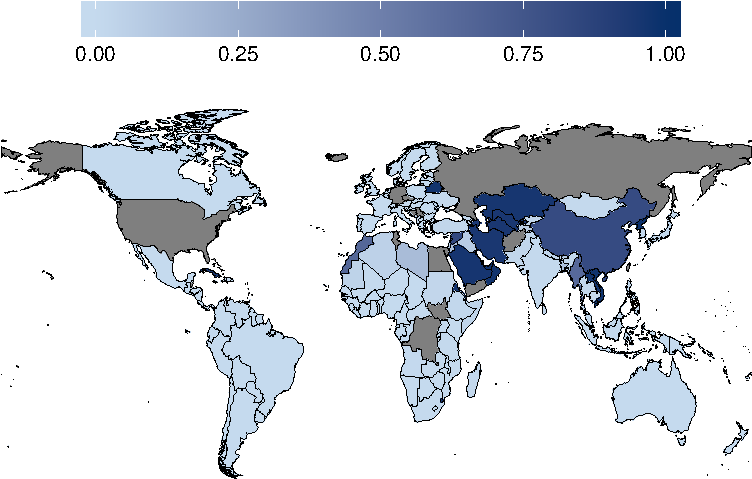
\includegraphics[width=.5\textwidth]{polCat_cat1_2012_map}
			\label{fig:mapp1}} &
		\subfloat[][-5 -- 0]{
			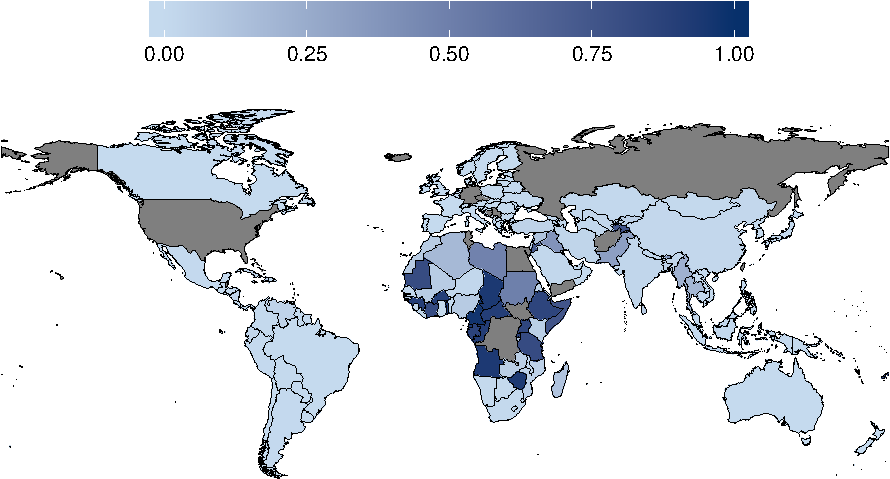
\includegraphics[width=.5\textwidth]{polCat_cat2_2012_map}
			\label{fig:mapp2}} \\
		\subfloat[][1 -- 5]{
			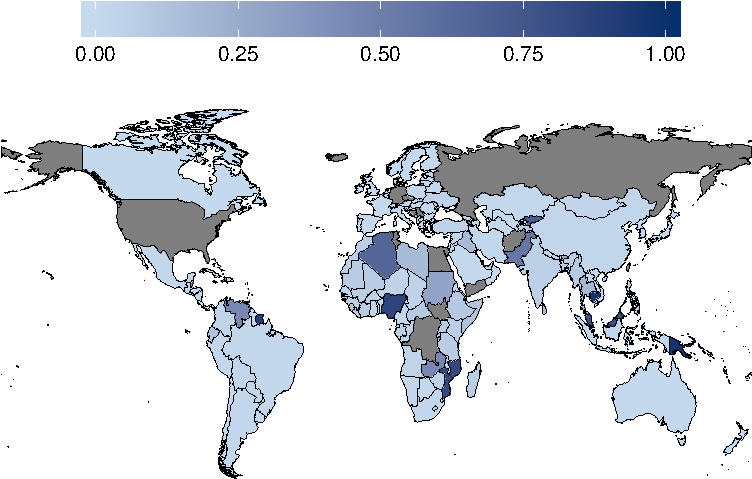
\includegraphics[width=.5\textwidth]{polCat_cat3_2012_map}
			\label{fig:mapp3}} &
		\subfloat[][6 -- 10]{
			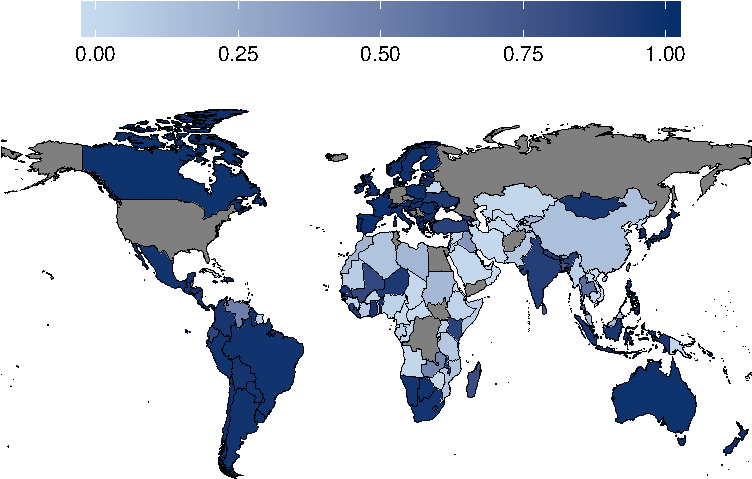
\includegraphics[width=.5\textwidth]{polCat_cat4_2012_map}
			\label{fig:mapp4}}
	\end{tabular}
\caption{Heat Maps of Out-of-Sample Confidence Scores from Support Vector Machines (SVM) of Four Regime Types.}
\end{figure}
\FloatBarrier

\begin{figure}[!t]
	\begin{tabular}{ll}
		\subfloat[][Military]{
			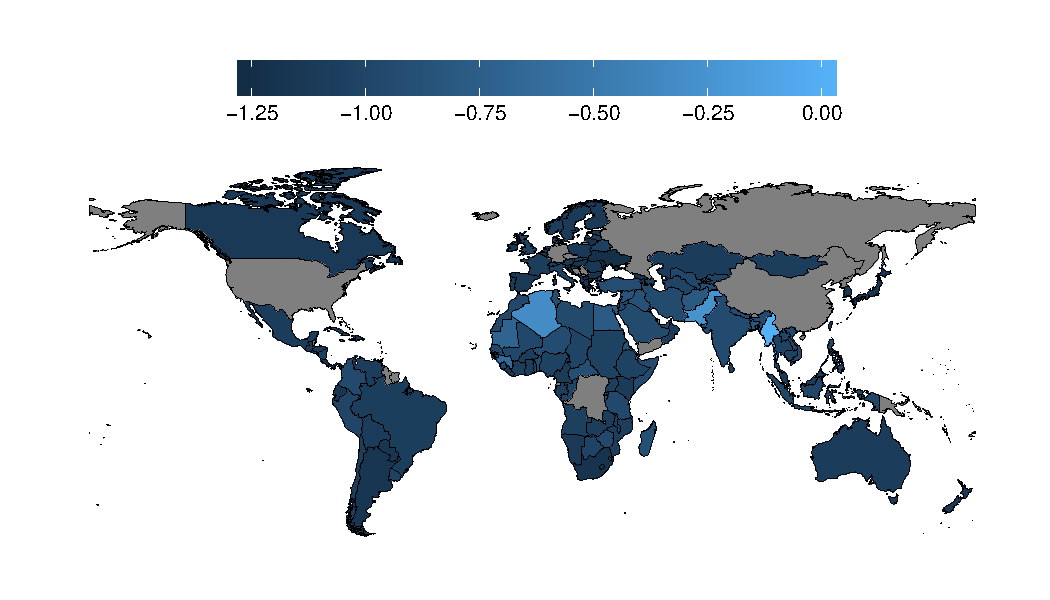
\includegraphics[width=.5\textwidth]{military_2010_map}
			\label{fig:mapmil}} &
		\subfloat[][Monarchy]{
			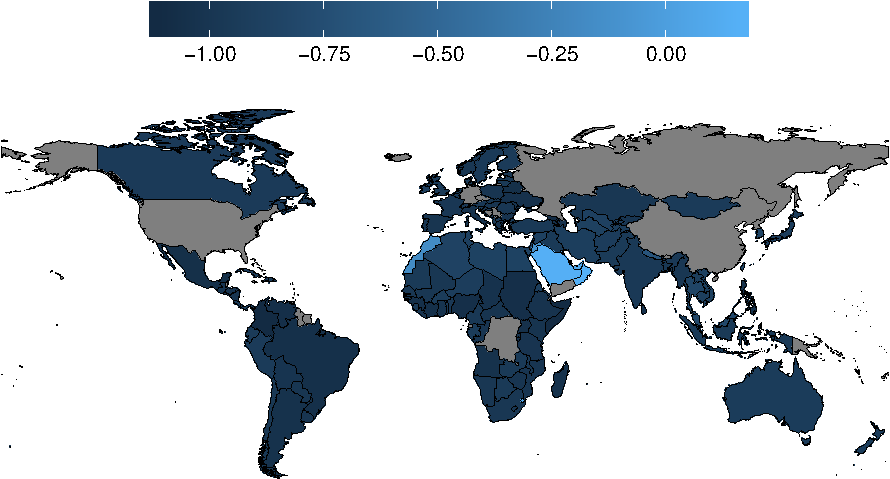
\includegraphics[width=.5\textwidth]{monarchy_2010_map}
			\label{fig:mapmon}} \\
		\subfloat[][Party]{
			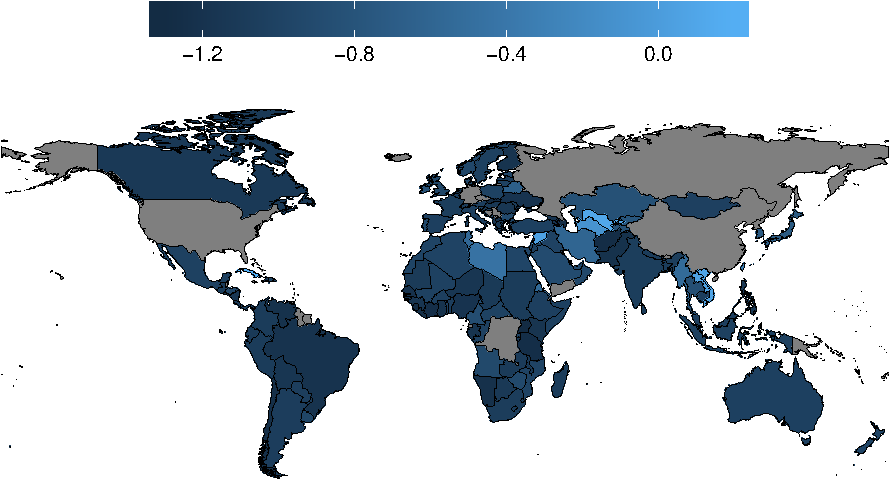
\includegraphics[width=.5\textwidth]{party_2010_map}
			\label{fig:mapparty}}
	\end{tabular}
\caption{Heat Maps of Out-of-Sample Confidence Scores from Support Vector Machines (SVM) of Four Regime Types.}
\end{figure}
\FloatBarrier

On the whole, cases fall out as we would expect them to. The results seem valid on their face. For example, the democracy classifier confidently identifies Western Europe, Canada, Australia, and New Zealand as democracies; shows interesting variations in Eastern Europe and Latin America; and confidently identifies nearly all of the rest of the world as non-democracies (defined for this task as a Polity score of 10). Meanwhile, the monarchy model correctly identifies most of the countries of the Arabian Peninsula, Jordan, and Morocco as monarchies and the rest of the world as not. The military rule classifier sees Myanmar, Pakistan, and (more surprisingly) Algeria as likely cases in 2010, and is less certain about the absence of military rule in several West African and Middle Eastern countries than in the rest of the world. The map of results from the one-party rule classifier is probably the least informative because it is missing data for a few critical cases, including China and North Korea. Still, it seems to do well with the rest of the world, including confident identification of one-party regimes in Syria, Vietnam, Laos, Turkmenistan, and Uzbekistan and midrange values for Iran, Kazakhstan, Libya, Eritrea, and Myanmar.

Also track changes over time

\begin{figure}[ht]
	\centering
	\resizebox{0.7\textwidth}{!}{% Created by tikzDevice version 0.7.0 on 2015-01-10 18:42:07
% !TEX encoding = UTF-8 Unicode
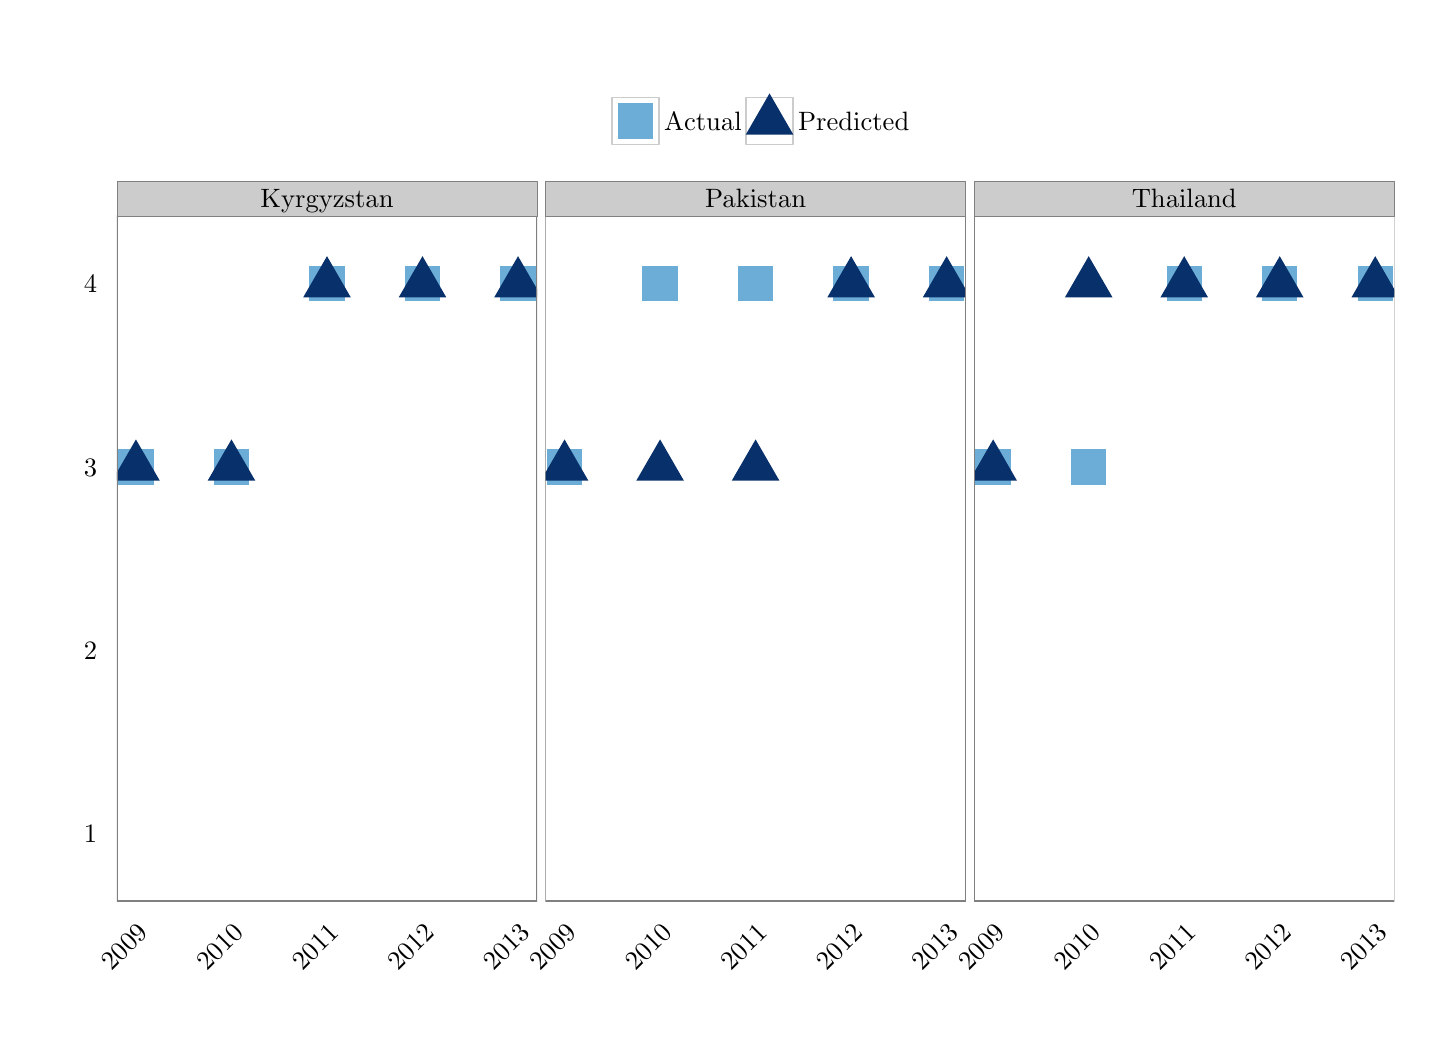
\begin{tikzpicture}[x=1pt,y=1pt]
\definecolor[named]{fillColor}{rgb}{1.00,1.00,1.00}
\path[use as bounding box,fill=fillColor,fill opacity=0.00] (0,0) rectangle (505.89,361.35);
\begin{scope}
\path[clip] (  0.00,  0.00) rectangle (505.89,361.35);
\definecolor[named]{drawColor}{rgb}{1.00,1.00,1.00}
\definecolor[named]{fillColor}{rgb}{1.00,1.00,1.00}

\path[draw=drawColor,line width= 0.6pt,line join=round,line cap=round,fill=fillColor] ( -0.00,  0.00) rectangle (505.89,361.35);
\end{scope}
\begin{scope}
\path[clip] ( 32.22, 45.67) rectangle (184.09,293.33);
\definecolor[named]{fillColor}{rgb}{1.00,1.00,1.00}

\path[fill=fillColor] ( 32.22, 45.67) rectangle (184.09,293.33);
\definecolor[named]{fillColor}{rgb}{0.42,0.68,0.84}

\path[fill=fillColor] (101.75,262.43) --
	(114.56,262.43) --
	(114.56,275.23) --
	(101.75,275.23) --
	cycle;

\path[fill=fillColor] ( 67.24,196.21) --
	( 80.04,196.21) --
	( 80.04,209.01) --
	( 67.24,209.01) --
	cycle;

\path[fill=fillColor] (170.78,262.43) --
	(183.59,262.43) --
	(183.59,275.23) --
	(170.78,275.23) --
	cycle;

\path[fill=fillColor] (136.27,262.43) --
	(149.07,262.43) --
	(149.07,275.23) --
	(136.27,275.23) --
	cycle;

\path[fill=fillColor] ( 32.72,196.21) --
	( 45.53,196.21) --
	( 45.53,209.01) --
	( 32.72,209.01) --
	cycle;
\definecolor[named]{fillColor}{rgb}{0.03,0.19,0.42}

\path[fill=fillColor] (108.16,278.78) --
	(116.78,263.85) --
	( 99.53,263.85) --
	cycle;

\path[fill=fillColor] ( 73.64,212.56) --
	( 82.26,197.63) --
	( 65.02,197.63) --
	cycle;

\path[fill=fillColor] (177.19,278.78) --
	(185.81,263.85) --
	(168.56,263.85) --
	cycle;

\path[fill=fillColor] (142.67,278.78) --
	(151.29,263.85) --
	(134.05,263.85) --
	cycle;

\path[fill=fillColor] ( 39.12,212.56) --
	( 47.75,197.63) --
	( 30.50,197.63) --
	cycle;
\definecolor[named]{drawColor}{rgb}{0.50,0.50,0.50}

\path[draw=drawColor,line width= 0.6pt,line join=round,line cap=round] ( 32.22, 45.67) rectangle (184.09,293.33);
\end{scope}
\begin{scope}
\path[clip] (187.10, 45.67) rectangle (338.97,293.33);
\definecolor[named]{fillColor}{rgb}{1.00,1.00,1.00}

\path[fill=fillColor] (187.10, 45.67) rectangle (338.97,293.33);
\definecolor[named]{fillColor}{rgb}{0.42,0.68,0.84}

\path[fill=fillColor] (256.63,262.43) --
	(269.44,262.43) --
	(269.44,275.23) --
	(256.63,275.23) --
	cycle;

\path[fill=fillColor] (187.60,196.21) --
	(200.40,196.21) --
	(200.40,209.01) --
	(187.60,209.01) --
	cycle;

\path[fill=fillColor] (222.12,262.43) --
	(234.92,262.43) --
	(234.92,275.23) --
	(222.12,275.23) --
	cycle;

\path[fill=fillColor] (291.15,262.43) --
	(303.95,262.43) --
	(303.95,275.23) --
	(291.15,275.23) --
	cycle;

\path[fill=fillColor] (325.66,262.43) --
	(338.47,262.43) --
	(338.47,275.23) --
	(325.66,275.23) --
	cycle;
\definecolor[named]{fillColor}{rgb}{0.03,0.19,0.42}

\path[fill=fillColor] (263.03,212.56) --
	(271.66,197.63) --
	(254.41,197.63) --
	cycle;

\path[fill=fillColor] (194.00,212.56) --
	(202.62,197.63) --
	(185.38,197.63) --
	cycle;

\path[fill=fillColor] (228.52,212.56) --
	(237.14,197.63) --
	(219.90,197.63) --
	cycle;

\path[fill=fillColor] (297.55,278.78) --
	(306.17,263.85) --
	(288.93,263.85) --
	cycle;

\path[fill=fillColor] (332.06,278.78) --
	(340.69,263.85) --
	(323.44,263.85) --
	cycle;
\definecolor[named]{drawColor}{rgb}{0.50,0.50,0.50}

\path[draw=drawColor,line width= 0.6pt,line join=round,line cap=round] (187.10, 45.67) rectangle (338.97,293.33);
\end{scope}
\begin{scope}
\path[clip] (341.98, 45.67) rectangle (493.85,293.33);
\definecolor[named]{fillColor}{rgb}{1.00,1.00,1.00}

\path[fill=fillColor] (341.98, 45.67) rectangle (493.85,293.33);
\definecolor[named]{fillColor}{rgb}{0.42,0.68,0.84}

\path[fill=fillColor] (376.99,196.21) --
	(389.80,196.21) --
	(389.80,209.01) --
	(376.99,209.01) --
	cycle;

\path[fill=fillColor] (411.51,262.43) --
	(424.31,262.43) --
	(424.31,275.23) --
	(411.51,275.23) --
	cycle;

\path[fill=fillColor] (446.02,262.43) --
	(458.83,262.43) --
	(458.83,275.23) --
	(446.02,275.23) --
	cycle;

\path[fill=fillColor] (480.54,262.43) --
	(493.34,262.43) --
	(493.34,275.23) --
	(480.54,275.23) --
	cycle;

\path[fill=fillColor] (342.48,196.21) --
	(355.28,196.21) --
	(355.28,209.01) --
	(342.48,209.01) --
	cycle;
\definecolor[named]{fillColor}{rgb}{0.03,0.19,0.42}

\path[fill=fillColor] (383.40,278.78) --
	(392.02,263.85) --
	(374.77,263.85) --
	cycle;

\path[fill=fillColor] (417.91,278.78) --
	(426.53,263.85) --
	(409.29,263.85) --
	cycle;

\path[fill=fillColor] (452.43,278.78) --
	(461.05,263.85) --
	(443.80,263.85) --
	cycle;

\path[fill=fillColor] (486.94,278.78) --
	(495.56,263.85) --
	(478.32,263.85) --
	cycle;

\path[fill=fillColor] (348.88,212.56) --
	(357.50,197.63) --
	(340.26,197.63) --
	cycle;
\definecolor[named]{drawColor}{rgb}{0.50,0.50,0.50}

\path[draw=drawColor,line width= 0.6pt,line join=round,line cap=round] (341.98, 45.67) rectangle (493.85,293.33);
\end{scope}
\begin{scope}
\path[clip] (  0.00,  0.00) rectangle (505.89,361.35);
\definecolor[named]{drawColor}{rgb}{0.50,0.50,0.50}
\definecolor[named]{fillColor}{rgb}{0.80,0.80,0.80}

\path[draw=drawColor,line width= 0.2pt,line join=round,line cap=round,fill=fillColor] ( 32.22,293.33) rectangle (184.09,305.96);
\definecolor[named]{drawColor}{rgb}{0.00,0.00,0.00}

\node[text=drawColor,anchor=base,inner sep=0pt, outer sep=0pt, scale=  0.96] at (108.16,296.34) {Kyrgyzstan};
\end{scope}
\begin{scope}
\path[clip] (  0.00,  0.00) rectangle (505.89,361.35);
\definecolor[named]{drawColor}{rgb}{0.50,0.50,0.50}
\definecolor[named]{fillColor}{rgb}{0.80,0.80,0.80}

\path[draw=drawColor,line width= 0.2pt,line join=round,line cap=round,fill=fillColor] (187.10,293.33) rectangle (338.97,305.96);
\definecolor[named]{drawColor}{rgb}{0.00,0.00,0.00}

\node[text=drawColor,anchor=base,inner sep=0pt, outer sep=0pt, scale=  0.96] at (263.03,296.34) {Pakistan};
\end{scope}
\begin{scope}
\path[clip] (  0.00,  0.00) rectangle (505.89,361.35);
\definecolor[named]{drawColor}{rgb}{0.50,0.50,0.50}
\definecolor[named]{fillColor}{rgb}{0.80,0.80,0.80}

\path[draw=drawColor,line width= 0.2pt,line join=round,line cap=round,fill=fillColor] (341.98,293.33) rectangle (493.85,305.96);
\definecolor[named]{drawColor}{rgb}{0.00,0.00,0.00}

\node[text=drawColor,anchor=base,inner sep=0pt, outer sep=0pt, scale=  0.96] at (417.91,296.34) {Thailand};
\end{scope}
\begin{scope}
\path[clip] (  0.00,  0.00) rectangle (505.89,361.35);
\definecolor[named]{drawColor}{rgb}{0.00,0.00,0.00}

\node[text=drawColor,anchor=base east,inner sep=0pt, outer sep=0pt, scale=  0.96] at ( 25.11, 66.87) {1};

\node[text=drawColor,anchor=base east,inner sep=0pt, outer sep=0pt, scale=  0.96] at ( 25.11,133.08) {2};

\node[text=drawColor,anchor=base east,inner sep=0pt, outer sep=0pt, scale=  0.96] at ( 25.11,199.30) {3};

\node[text=drawColor,anchor=base east,inner sep=0pt, outer sep=0pt, scale=  0.96] at ( 25.11,265.52) {4};
\end{scope}
\begin{scope}
\path[clip] (  0.00,  0.00) rectangle (505.89,361.35);
\definecolor[named]{drawColor}{rgb}{0.00,0.00,0.00}

\node[text=drawColor,rotate= 45.00,anchor=base east,inner sep=0pt, outer sep=0pt, scale=  0.96] at ( 43.80, 33.88) {2009};

\node[text=drawColor,rotate= 45.00,anchor=base east,inner sep=0pt, outer sep=0pt, scale=  0.96] at ( 78.32, 33.88) {2010};

\node[text=drawColor,rotate= 45.00,anchor=base east,inner sep=0pt, outer sep=0pt, scale=  0.96] at (112.83, 33.88) {2011};

\node[text=drawColor,rotate= 45.00,anchor=base east,inner sep=0pt, outer sep=0pt, scale=  0.96] at (147.35, 33.88) {2012};

\node[text=drawColor,rotate= 45.00,anchor=base east,inner sep=0pt, outer sep=0pt, scale=  0.96] at (181.86, 33.88) {2013};
\end{scope}
\begin{scope}
\path[clip] (  0.00,  0.00) rectangle (505.89,361.35);
\definecolor[named]{drawColor}{rgb}{0.00,0.00,0.00}

\node[text=drawColor,rotate= 45.00,anchor=base east,inner sep=0pt, outer sep=0pt, scale=  0.96] at (198.68, 33.88) {2009};

\node[text=drawColor,rotate= 45.00,anchor=base east,inner sep=0pt, outer sep=0pt, scale=  0.96] at (233.19, 33.88) {2010};

\node[text=drawColor,rotate= 45.00,anchor=base east,inner sep=0pt, outer sep=0pt, scale=  0.96] at (267.71, 33.88) {2011};

\node[text=drawColor,rotate= 45.00,anchor=base east,inner sep=0pt, outer sep=0pt, scale=  0.96] at (302.22, 33.88) {2012};

\node[text=drawColor,rotate= 45.00,anchor=base east,inner sep=0pt, outer sep=0pt, scale=  0.96] at (336.74, 33.88) {2013};
\end{scope}
\begin{scope}
\path[clip] (  0.00,  0.00) rectangle (505.89,361.35);
\definecolor[named]{drawColor}{rgb}{0.00,0.00,0.00}

\node[text=drawColor,rotate= 45.00,anchor=base east,inner sep=0pt, outer sep=0pt, scale=  0.96] at (353.56, 33.88) {2009};

\node[text=drawColor,rotate= 45.00,anchor=base east,inner sep=0pt, outer sep=0pt, scale=  0.96] at (388.07, 33.88) {2010};

\node[text=drawColor,rotate= 45.00,anchor=base east,inner sep=0pt, outer sep=0pt, scale=  0.96] at (422.59, 33.88) {2011};

\node[text=drawColor,rotate= 45.00,anchor=base east,inner sep=0pt, outer sep=0pt, scale=  0.96] at (457.10, 33.88) {2012};

\node[text=drawColor,rotate= 45.00,anchor=base east,inner sep=0pt, outer sep=0pt, scale=  0.96] at (491.62, 33.88) {2013};
\end{scope}
\begin{scope}
\path[clip] (  0.00,  0.00) rectangle (505.89,361.35);
\definecolor[named]{fillColor}{rgb}{1.00,1.00,1.00}

\path[fill=fillColor] (203.24,314.83) rectangle (322.83,340.44);
\end{scope}
\begin{scope}
\path[clip] (  0.00,  0.00) rectangle (505.89,361.35);
\definecolor[named]{drawColor}{rgb}{0.80,0.80,0.80}
\definecolor[named]{fillColor}{rgb}{1.00,1.00,1.00}

\path[draw=drawColor,line width= 0.6pt,line join=round,line cap=round,fill=fillColor] (211.12,319.10) rectangle (228.19,336.17);
\end{scope}
\begin{scope}
\path[clip] (  0.00,  0.00) rectangle (505.89,361.35);
\definecolor[named]{fillColor}{rgb}{0.42,0.68,0.84}

\path[fill=fillColor] (213.25,321.23) --
	(226.06,321.23) --
	(226.06,334.04) --
	(213.25,334.04) --
	cycle;
\end{scope}
\begin{scope}
\path[clip] (  0.00,  0.00) rectangle (505.89,361.35);
\definecolor[named]{drawColor}{rgb}{0.80,0.80,0.80}
\definecolor[named]{fillColor}{rgb}{1.00,1.00,1.00}

\path[draw=drawColor,line width= 0.6pt,line join=round,line cap=round,fill=fillColor] (259.53,319.10) rectangle (276.60,336.17);
\end{scope}
\begin{scope}
\path[clip] (  0.00,  0.00) rectangle (505.89,361.35);
\definecolor[named]{fillColor}{rgb}{0.03,0.19,0.42}

\path[fill=fillColor] (268.07,337.59) --
	(276.69,322.66) --
	(259.45,322.66) --
	cycle;
\end{scope}
\begin{scope}
\path[clip] (  0.00,  0.00) rectangle (505.89,361.35);
\definecolor[named]{drawColor}{rgb}{0.00,0.00,0.00}

\node[text=drawColor,anchor=base west,inner sep=0pt, outer sep=0pt, scale=  0.96] at (230.00,324.33) {Actual};
\end{scope}
\begin{scope}
\path[clip] (  0.00,  0.00) rectangle (505.89,361.35);
\definecolor[named]{drawColor}{rgb}{0.00,0.00,0.00}

\node[text=drawColor,anchor=base west,inner sep=0pt, outer sep=0pt, scale=  0.96] at (278.41,324.33) {Predicted};
\end{scope}
\end{tikzpicture}
}	
	\caption{Histograms of Out-of-Sample Estimated Probabilities of Four Regime Types from Support Vector Machines (SVM)}
\end{figure}

\begin{figure}[ht]
	\centering
	\resizebox{0.7\textwidth}{!}{% Created by tikzDevice version 0.7.0 on 2015-01-10 18:42:07
% !TEX encoding = UTF-8 Unicode
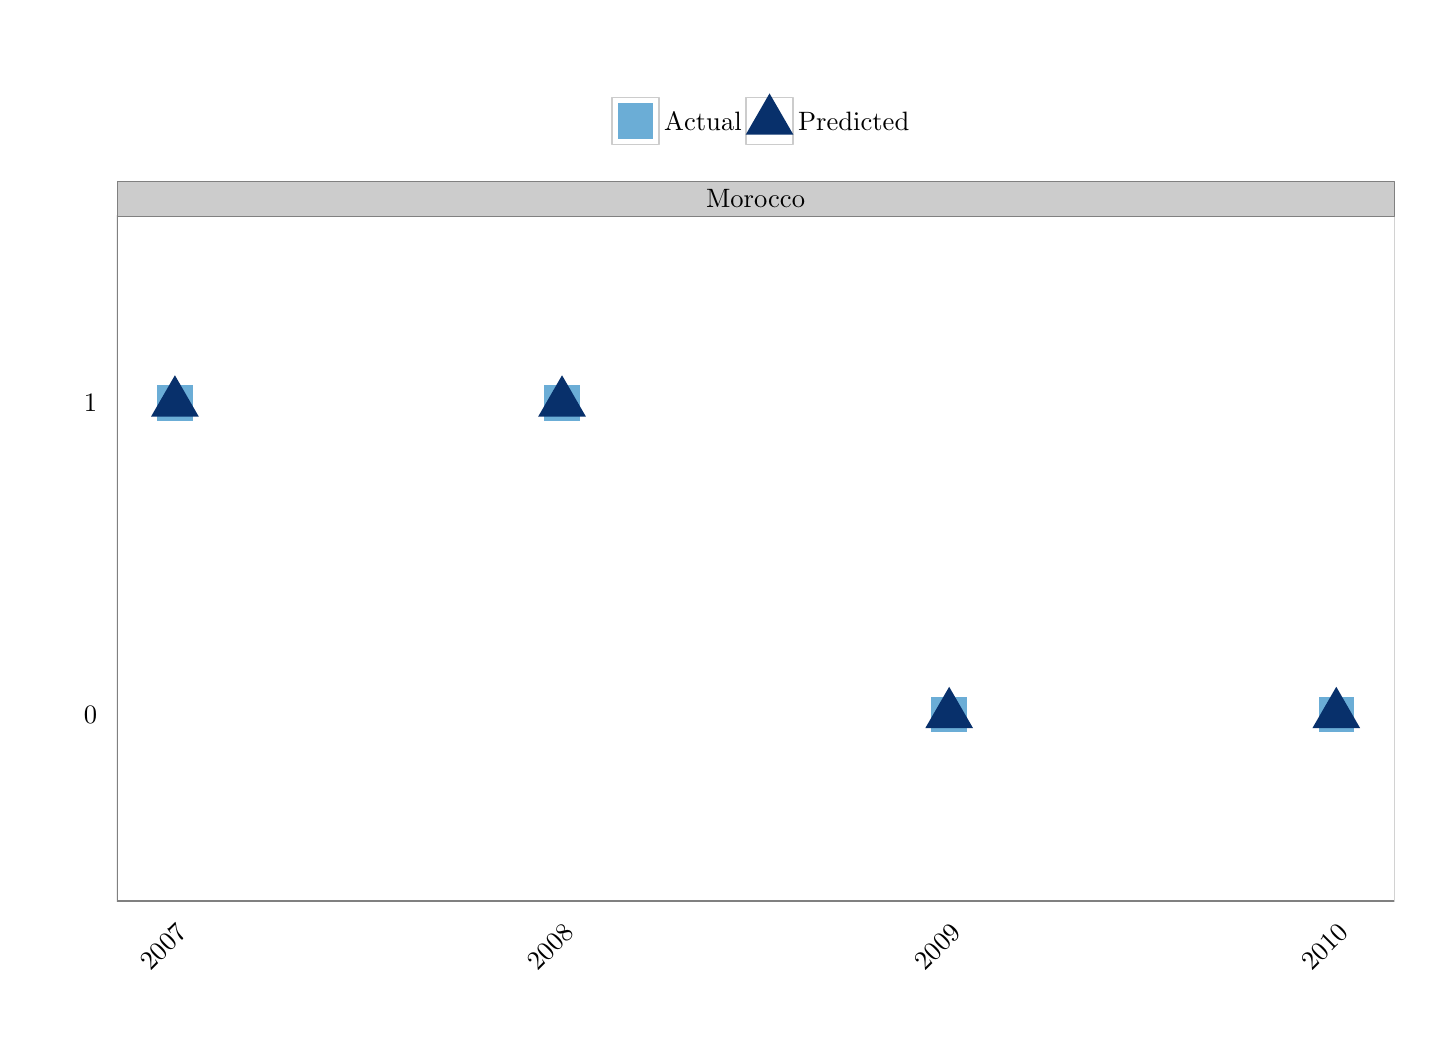
\begin{tikzpicture}[x=1pt,y=1pt]
\definecolor[named]{fillColor}{rgb}{1.00,1.00,1.00}
\path[use as bounding box,fill=fillColor,fill opacity=0.00] (0,0) rectangle (505.89,361.35);
\begin{scope}
\path[clip] (  0.00,  0.00) rectangle (505.89,361.35);
\definecolor[named]{drawColor}{rgb}{1.00,1.00,1.00}
\definecolor[named]{fillColor}{rgb}{1.00,1.00,1.00}

\path[draw=drawColor,line width= 0.6pt,line join=round,line cap=round,fill=fillColor] (  0.00,  0.00) rectangle (505.89,361.35);
\end{scope}
\begin{scope}
\path[clip] ( 32.22, 45.67) rectangle (493.85,293.33);
\definecolor[named]{fillColor}{rgb}{1.00,1.00,1.00}

\path[fill=fillColor] ( 32.22, 45.67) rectangle (493.85,293.33);
\definecolor[named]{fillColor}{rgb}{0.42,0.68,0.84}

\path[fill=fillColor] (466.46,106.81) --
	(479.26,106.81) --
	(479.26,119.62) --
	(466.46,119.62) --
	cycle;

\path[fill=fillColor] (326.57,106.81) --
	(339.38,106.81) --
	(339.38,119.62) --
	(326.57,119.62) --
	cycle;

\path[fill=fillColor] (186.69,219.38) --
	(199.49,219.38) --
	(199.49,232.19) --
	(186.69,232.19) --
	cycle;

\path[fill=fillColor] ( 46.80,219.38) --
	( 59.61,219.38) --
	( 59.61,232.19) --
	( 46.80,232.19) --
	cycle;
\definecolor[named]{fillColor}{rgb}{0.03,0.19,0.42}

\path[fill=fillColor] (472.86,123.17) --
	(481.48,108.24) --
	(464.24,108.24) --
	cycle;

\path[fill=fillColor] (332.98,123.17) --
	(341.60,108.24) --
	(324.35,108.24) --
	cycle;

\path[fill=fillColor] (193.09,235.74) --
	(201.71,220.81) --
	(184.47,220.81) --
	cycle;

\path[fill=fillColor] ( 53.20,235.74) --
	( 61.83,220.81) --
	( 44.58,220.81) --
	cycle;
\definecolor[named]{drawColor}{rgb}{0.50,0.50,0.50}

\path[draw=drawColor,line width= 0.6pt,line join=round,line cap=round] ( 32.22, 45.67) rectangle (493.85,293.33);
\end{scope}
\begin{scope}
\path[clip] (  0.00,  0.00) rectangle (505.89,361.35);
\definecolor[named]{drawColor}{rgb}{0.50,0.50,0.50}
\definecolor[named]{fillColor}{rgb}{0.80,0.80,0.80}

\path[draw=drawColor,line width= 0.2pt,line join=round,line cap=round,fill=fillColor] ( 32.22,293.33) rectangle (493.85,305.96);
\definecolor[named]{drawColor}{rgb}{0.00,0.00,0.00}

\node[text=drawColor,anchor=base,inner sep=0pt, outer sep=0pt, scale=  0.96] at (263.03,296.34) {Morocco};
\end{scope}
\begin{scope}
\path[clip] (  0.00,  0.00) rectangle (505.89,361.35);
\definecolor[named]{drawColor}{rgb}{0.00,0.00,0.00}

\node[text=drawColor,anchor=base east,inner sep=0pt, outer sep=0pt, scale=  0.96] at ( 25.11,109.91) {0};

\node[text=drawColor,anchor=base east,inner sep=0pt, outer sep=0pt, scale=  0.96] at ( 25.11,222.48) {1};
\end{scope}
\begin{scope}
\path[clip] (  0.00,  0.00) rectangle (505.89,361.35);
\definecolor[named]{drawColor}{rgb}{0.00,0.00,0.00}

\node[text=drawColor,rotate= 45.00,anchor=base east,inner sep=0pt, outer sep=0pt, scale=  0.96] at ( 57.88, 33.88) {2007};

\node[text=drawColor,rotate= 45.00,anchor=base east,inner sep=0pt, outer sep=0pt, scale=  0.96] at (197.77, 33.88) {2008};

\node[text=drawColor,rotate= 45.00,anchor=base east,inner sep=0pt, outer sep=0pt, scale=  0.96] at (337.65, 33.88) {2009};

\node[text=drawColor,rotate= 45.00,anchor=base east,inner sep=0pt, outer sep=0pt, scale=  0.96] at (477.54, 33.88) {2010};
\end{scope}
\begin{scope}
\path[clip] (  0.00,  0.00) rectangle (505.89,361.35);
\definecolor[named]{fillColor}{rgb}{1.00,1.00,1.00}

\path[fill=fillColor] (203.24,314.83) rectangle (322.83,340.44);
\end{scope}
\begin{scope}
\path[clip] (  0.00,  0.00) rectangle (505.89,361.35);
\definecolor[named]{drawColor}{rgb}{0.80,0.80,0.80}
\definecolor[named]{fillColor}{rgb}{1.00,1.00,1.00}

\path[draw=drawColor,line width= 0.6pt,line join=round,line cap=round,fill=fillColor] (211.12,319.10) rectangle (228.19,336.17);
\end{scope}
\begin{scope}
\path[clip] (  0.00,  0.00) rectangle (505.89,361.35);
\definecolor[named]{fillColor}{rgb}{0.42,0.68,0.84}

\path[fill=fillColor] (213.25,321.23) --
	(226.06,321.23) --
	(226.06,334.04) --
	(213.25,334.04) --
	cycle;
\end{scope}
\begin{scope}
\path[clip] (  0.00,  0.00) rectangle (505.89,361.35);
\definecolor[named]{drawColor}{rgb}{0.80,0.80,0.80}
\definecolor[named]{fillColor}{rgb}{1.00,1.00,1.00}

\path[draw=drawColor,line width= 0.6pt,line join=round,line cap=round,fill=fillColor] (259.53,319.10) rectangle (276.60,336.17);
\end{scope}
\begin{scope}
\path[clip] (  0.00,  0.00) rectangle (505.89,361.35);
\definecolor[named]{fillColor}{rgb}{0.03,0.19,0.42}

\path[fill=fillColor] (268.07,337.59) --
	(276.69,322.66) --
	(259.45,322.66) --
	cycle;
\end{scope}
\begin{scope}
\path[clip] (  0.00,  0.00) rectangle (505.89,361.35);
\definecolor[named]{drawColor}{rgb}{0.00,0.00,0.00}

\node[text=drawColor,anchor=base west,inner sep=0pt, outer sep=0pt, scale=  0.96] at (230.00,324.33) {Actual};
\end{scope}
\begin{scope}
\path[clip] (  0.00,  0.00) rectangle (505.89,361.35);
\definecolor[named]{drawColor}{rgb}{0.00,0.00,0.00}

\node[text=drawColor,anchor=base west,inner sep=0pt, outer sep=0pt, scale=  0.96] at (278.41,324.33) {Predicted};
\end{scope}
\end{tikzpicture}
}	
	\caption{Histograms of Out-of-Sample Estimated Probabilities of Four Regime Types from Support Vector Machines (SVM)}
\end{figure}

\begin{figure}[ht]
	\centering
	\resizebox{0.7\textwidth}{!}{% Created by tikzDevice version 0.7.0 on 2015-01-10 18:42:08
% !TEX encoding = UTF-8 Unicode
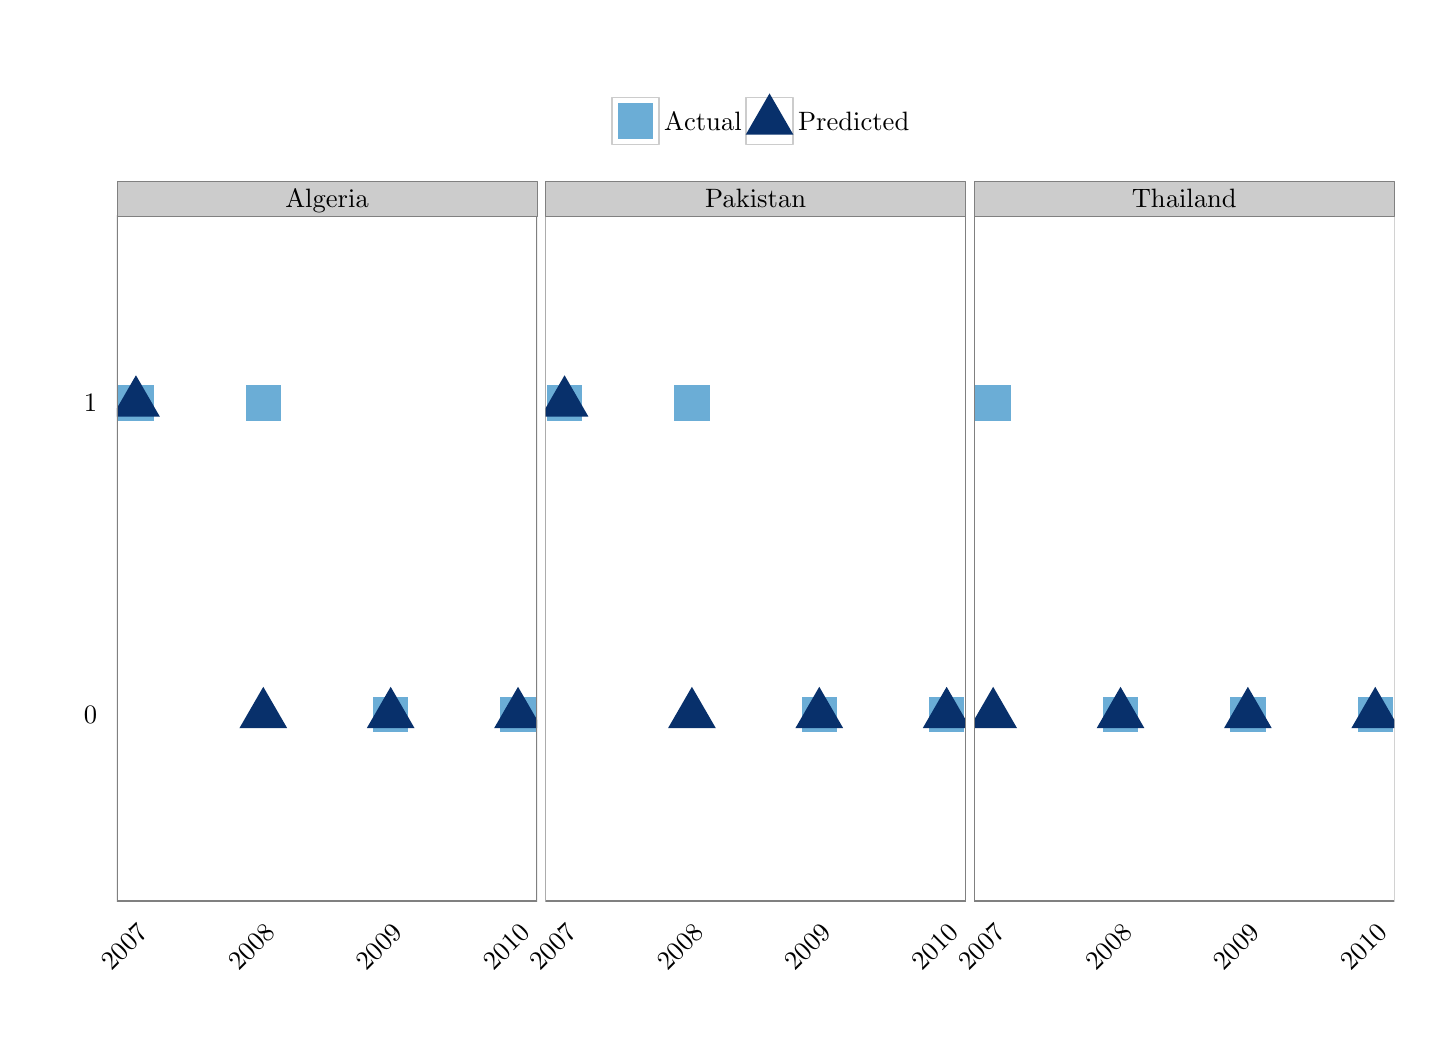
\begin{tikzpicture}[x=1pt,y=1pt]
\definecolor[named]{fillColor}{rgb}{1.00,1.00,1.00}
\path[use as bounding box,fill=fillColor,fill opacity=0.00] (0,0) rectangle (505.89,361.35);
\begin{scope}
\path[clip] (  0.00,  0.00) rectangle (505.89,361.35);
\definecolor[named]{drawColor}{rgb}{1.00,1.00,1.00}
\definecolor[named]{fillColor}{rgb}{1.00,1.00,1.00}

\path[draw=drawColor,line width= 0.6pt,line join=round,line cap=round,fill=fillColor] ( -0.00,  0.00) rectangle (505.89,361.35);
\end{scope}
\begin{scope}
\path[clip] ( 32.22, 45.67) rectangle (184.09,293.33);
\definecolor[named]{fillColor}{rgb}{1.00,1.00,1.00}

\path[fill=fillColor] ( 32.22, 45.67) rectangle (184.09,293.33);
\definecolor[named]{fillColor}{rgb}{0.42,0.68,0.84}

\path[fill=fillColor] ( 78.74,219.38) --
	( 91.55,219.38) --
	( 91.55,232.19) --
	( 78.74,232.19) --
	cycle;

\path[fill=fillColor] ( 32.72,219.38) --
	( 45.53,219.38) --
	( 45.53,232.19) --
	( 32.72,232.19) --
	cycle;

\path[fill=fillColor] (124.76,106.81) --
	(137.57,106.81) --
	(137.57,119.62) --
	(124.76,119.62) --
	cycle;

\path[fill=fillColor] (170.78,106.81) --
	(183.59,106.81) --
	(183.59,119.62) --
	(170.78,119.62) --
	cycle;
\definecolor[named]{fillColor}{rgb}{0.03,0.19,0.42}

\path[fill=fillColor] ( 85.14,123.17) --
	( 93.77,108.24) --
	( 76.52,108.24) --
	cycle;

\path[fill=fillColor] ( 39.12,235.74) --
	( 47.75,220.81) --
	( 30.50,220.81) --
	cycle;

\path[fill=fillColor] (131.17,123.17) --
	(139.79,108.24) --
	(122.54,108.24) --
	cycle;

\path[fill=fillColor] (177.19,123.17) --
	(185.81,108.24) --
	(168.56,108.24) --
	cycle;
\definecolor[named]{drawColor}{rgb}{0.50,0.50,0.50}

\path[draw=drawColor,line width= 0.6pt,line join=round,line cap=round] ( 32.22, 45.67) rectangle (184.09,293.33);
\end{scope}
\begin{scope}
\path[clip] (187.10, 45.67) rectangle (338.97,293.33);
\definecolor[named]{fillColor}{rgb}{1.00,1.00,1.00}

\path[fill=fillColor] (187.10, 45.67) rectangle (338.97,293.33);
\definecolor[named]{fillColor}{rgb}{0.42,0.68,0.84}

\path[fill=fillColor] (187.60,219.38) --
	(200.40,219.38) --
	(200.40,232.19) --
	(187.60,232.19) --
	cycle;

\path[fill=fillColor] (279.64,106.81) --
	(292.45,106.81) --
	(292.45,119.62) --
	(279.64,119.62) --
	cycle;

\path[fill=fillColor] (233.62,219.38) --
	(246.43,219.38) --
	(246.43,232.19) --
	(233.62,232.19) --
	cycle;

\path[fill=fillColor] (325.66,106.81) --
	(338.47,106.81) --
	(338.47,119.62) --
	(325.66,119.62) --
	cycle;
\definecolor[named]{fillColor}{rgb}{0.03,0.19,0.42}

\path[fill=fillColor] (194.00,235.74) --
	(202.62,220.81) --
	(185.38,220.81) --
	cycle;

\path[fill=fillColor] (286.04,123.17) --
	(294.67,108.24) --
	(277.42,108.24) --
	cycle;

\path[fill=fillColor] (240.02,123.17) --
	(248.65,108.24) --
	(231.40,108.24) --
	cycle;

\path[fill=fillColor] (332.06,123.17) --
	(340.69,108.24) --
	(323.44,108.24) --
	cycle;
\definecolor[named]{drawColor}{rgb}{0.50,0.50,0.50}

\path[draw=drawColor,line width= 0.6pt,line join=round,line cap=round] (187.10, 45.67) rectangle (338.97,293.33);
\end{scope}
\begin{scope}
\path[clip] (341.98, 45.67) rectangle (493.85,293.33);
\definecolor[named]{fillColor}{rgb}{1.00,1.00,1.00}

\path[fill=fillColor] (341.98, 45.67) rectangle (493.85,293.33);
\definecolor[named]{fillColor}{rgb}{0.42,0.68,0.84}

\path[fill=fillColor] (480.54,106.81) --
	(493.34,106.81) --
	(493.34,119.62) --
	(480.54,119.62) --
	cycle;

\path[fill=fillColor] (434.52,106.81) --
	(447.32,106.81) --
	(447.32,119.62) --
	(434.52,119.62) --
	cycle;

\path[fill=fillColor] (388.50,106.81) --
	(401.30,106.81) --
	(401.30,119.62) --
	(388.50,119.62) --
	cycle;

\path[fill=fillColor] (342.48,219.38) --
	(355.28,219.38) --
	(355.28,232.19) --
	(342.48,232.19) --
	cycle;
\definecolor[named]{fillColor}{rgb}{0.03,0.19,0.42}

\path[fill=fillColor] (486.94,123.17) --
	(495.56,108.24) --
	(478.32,108.24) --
	cycle;

\path[fill=fillColor] (440.92,123.17) --
	(449.54,108.24) --
	(432.30,108.24) --
	cycle;

\path[fill=fillColor] (394.90,123.17) --
	(403.52,108.24) --
	(386.28,108.24) --
	cycle;

\path[fill=fillColor] (348.88,123.17) --
	(357.50,108.24) --
	(340.26,108.24) --
	cycle;
\definecolor[named]{drawColor}{rgb}{0.50,0.50,0.50}

\path[draw=drawColor,line width= 0.6pt,line join=round,line cap=round] (341.98, 45.67) rectangle (493.85,293.33);
\end{scope}
\begin{scope}
\path[clip] (  0.00,  0.00) rectangle (505.89,361.35);
\definecolor[named]{drawColor}{rgb}{0.50,0.50,0.50}
\definecolor[named]{fillColor}{rgb}{0.80,0.80,0.80}

\path[draw=drawColor,line width= 0.2pt,line join=round,line cap=round,fill=fillColor] ( 32.22,293.33) rectangle (184.09,305.96);
\definecolor[named]{drawColor}{rgb}{0.00,0.00,0.00}

\node[text=drawColor,anchor=base,inner sep=0pt, outer sep=0pt, scale=  0.96] at (108.16,296.34) {Algeria};
\end{scope}
\begin{scope}
\path[clip] (  0.00,  0.00) rectangle (505.89,361.35);
\definecolor[named]{drawColor}{rgb}{0.50,0.50,0.50}
\definecolor[named]{fillColor}{rgb}{0.80,0.80,0.80}

\path[draw=drawColor,line width= 0.2pt,line join=round,line cap=round,fill=fillColor] (187.10,293.33) rectangle (338.97,305.96);
\definecolor[named]{drawColor}{rgb}{0.00,0.00,0.00}

\node[text=drawColor,anchor=base,inner sep=0pt, outer sep=0pt, scale=  0.96] at (263.03,296.34) {Pakistan};
\end{scope}
\begin{scope}
\path[clip] (  0.00,  0.00) rectangle (505.89,361.35);
\definecolor[named]{drawColor}{rgb}{0.50,0.50,0.50}
\definecolor[named]{fillColor}{rgb}{0.80,0.80,0.80}

\path[draw=drawColor,line width= 0.2pt,line join=round,line cap=round,fill=fillColor] (341.98,293.33) rectangle (493.85,305.96);
\definecolor[named]{drawColor}{rgb}{0.00,0.00,0.00}

\node[text=drawColor,anchor=base,inner sep=0pt, outer sep=0pt, scale=  0.96] at (417.91,296.34) {Thailand};
\end{scope}
\begin{scope}
\path[clip] (  0.00,  0.00) rectangle (505.89,361.35);
\definecolor[named]{drawColor}{rgb}{0.00,0.00,0.00}

\node[text=drawColor,anchor=base east,inner sep=0pt, outer sep=0pt, scale=  0.96] at ( 25.11,109.91) {0};

\node[text=drawColor,anchor=base east,inner sep=0pt, outer sep=0pt, scale=  0.96] at ( 25.11,222.48) {1};
\end{scope}
\begin{scope}
\path[clip] (  0.00,  0.00) rectangle (505.89,361.35);
\definecolor[named]{drawColor}{rgb}{0.00,0.00,0.00}

\node[text=drawColor,rotate= 45.00,anchor=base east,inner sep=0pt, outer sep=0pt, scale=  0.96] at ( 43.80, 33.88) {2007};

\node[text=drawColor,rotate= 45.00,anchor=base east,inner sep=0pt, outer sep=0pt, scale=  0.96] at ( 89.82, 33.88) {2008};

\node[text=drawColor,rotate= 45.00,anchor=base east,inner sep=0pt, outer sep=0pt, scale=  0.96] at (135.84, 33.88) {2009};

\node[text=drawColor,rotate= 45.00,anchor=base east,inner sep=0pt, outer sep=0pt, scale=  0.96] at (181.86, 33.88) {2010};
\end{scope}
\begin{scope}
\path[clip] (  0.00,  0.00) rectangle (505.89,361.35);
\definecolor[named]{drawColor}{rgb}{0.00,0.00,0.00}

\node[text=drawColor,rotate= 45.00,anchor=base east,inner sep=0pt, outer sep=0pt, scale=  0.96] at (198.68, 33.88) {2007};

\node[text=drawColor,rotate= 45.00,anchor=base east,inner sep=0pt, outer sep=0pt, scale=  0.96] at (244.70, 33.88) {2008};

\node[text=drawColor,rotate= 45.00,anchor=base east,inner sep=0pt, outer sep=0pt, scale=  0.96] at (290.72, 33.88) {2009};

\node[text=drawColor,rotate= 45.00,anchor=base east,inner sep=0pt, outer sep=0pt, scale=  0.96] at (336.74, 33.88) {2010};
\end{scope}
\begin{scope}
\path[clip] (  0.00,  0.00) rectangle (505.89,361.35);
\definecolor[named]{drawColor}{rgb}{0.00,0.00,0.00}

\node[text=drawColor,rotate= 45.00,anchor=base east,inner sep=0pt, outer sep=0pt, scale=  0.96] at (353.56, 33.88) {2007};

\node[text=drawColor,rotate= 45.00,anchor=base east,inner sep=0pt, outer sep=0pt, scale=  0.96] at (399.58, 33.88) {2008};

\node[text=drawColor,rotate= 45.00,anchor=base east,inner sep=0pt, outer sep=0pt, scale=  0.96] at (445.60, 33.88) {2009};

\node[text=drawColor,rotate= 45.00,anchor=base east,inner sep=0pt, outer sep=0pt, scale=  0.96] at (491.62, 33.88) {2010};
\end{scope}
\begin{scope}
\path[clip] (  0.00,  0.00) rectangle (505.89,361.35);
\definecolor[named]{fillColor}{rgb}{1.00,1.00,1.00}

\path[fill=fillColor] (203.24,314.83) rectangle (322.83,340.44);
\end{scope}
\begin{scope}
\path[clip] (  0.00,  0.00) rectangle (505.89,361.35);
\definecolor[named]{drawColor}{rgb}{0.80,0.80,0.80}
\definecolor[named]{fillColor}{rgb}{1.00,1.00,1.00}

\path[draw=drawColor,line width= 0.6pt,line join=round,line cap=round,fill=fillColor] (211.12,319.10) rectangle (228.19,336.17);
\end{scope}
\begin{scope}
\path[clip] (  0.00,  0.00) rectangle (505.89,361.35);
\definecolor[named]{fillColor}{rgb}{0.42,0.68,0.84}

\path[fill=fillColor] (213.25,321.23) --
	(226.06,321.23) --
	(226.06,334.04) --
	(213.25,334.04) --
	cycle;
\end{scope}
\begin{scope}
\path[clip] (  0.00,  0.00) rectangle (505.89,361.35);
\definecolor[named]{drawColor}{rgb}{0.80,0.80,0.80}
\definecolor[named]{fillColor}{rgb}{1.00,1.00,1.00}

\path[draw=drawColor,line width= 0.6pt,line join=round,line cap=round,fill=fillColor] (259.53,319.10) rectangle (276.60,336.17);
\end{scope}
\begin{scope}
\path[clip] (  0.00,  0.00) rectangle (505.89,361.35);
\definecolor[named]{fillColor}{rgb}{0.03,0.19,0.42}

\path[fill=fillColor] (268.07,337.59) --
	(276.69,322.66) --
	(259.45,322.66) --
	cycle;
\end{scope}
\begin{scope}
\path[clip] (  0.00,  0.00) rectangle (505.89,361.35);
\definecolor[named]{drawColor}{rgb}{0.00,0.00,0.00}

\node[text=drawColor,anchor=base west,inner sep=0pt, outer sep=0pt, scale=  0.96] at (230.00,324.33) {Actual};
\end{scope}
\begin{scope}
\path[clip] (  0.00,  0.00) rectangle (505.89,361.35);
\definecolor[named]{drawColor}{rgb}{0.00,0.00,0.00}

\node[text=drawColor,anchor=base west,inner sep=0pt, outer sep=0pt, scale=  0.96] at (278.41,324.33) {Predicted};
\end{scope}
\end{tikzpicture}
}	
	\caption{Histograms of Out-of-Sample Estimated Probabilities of Four Regime Types from Support Vector Machines (SVM)}
\end{figure}

\section{Conclusion}

The results described here demonstrate that it is possible to generate useful fuzzy-set measures of political regime type from publicly available texts at relatively low cost. An initial application using features derived from a small and corpus produced out-of-sample estimates that closely match observed data on several very different regime types.

The out-of-sample classification accuracy of our models is very good, but that doesn't mean we are satisfied with the output and ready to move to data production. We have two main concerns about the results of this initial implementation. First, the texts included in the relatively small corpus we have assembled so far only cover a narrow set of human-rights practices and political procedures. These practices and procedures are all fundamental to how we conceive and observe political regime type, but they aren't the only things that are.

To address this issue in future iterations, we plan to expand the corpus to include annual or occasional reports that discuss a broader range of features in each country's national politics. Eventually, we hope to add news stories to the mix. If we can develop models that perform well on an amalgamation of occasional reports and news stories, we will be able to implement this process in near-real time, constantly updating probabilistic measures of regime type for all countries of the world at very low cost.

Second, the stringent criteria we used to observe each regime type in constructing the binary indicators on which the classifiers are trained also appear to be shaping the results in undesirable ways. We started this project with a belief that membership in these regime categories is inherently fuzzy, and we are trying to build a process that uses text mining to estimate degrees of membership in those fuzzy sets. If set membership is inherently ambiguous in a fair number of cases, then our approximation of a membership function should be bimodal, but not too neatly so. Most cases most of the time can be placed confidently at one end of the range of degrees of membership or the other, but there is considerable uncertainty at any moment in time about a non-trivial number of cases, and our estimates should reflect that fact.

If that's right, then our initial estimates are probably too tidy, and we suspect that the stringent operationalization of each regime type in the training data is partly to blame.  To address this problem in future iterations, we hope to experiment with two alternatives. First, we may lower the bar for observed membership in each category in the training data. For example, we could lower the Polity threshold for observing democracy from 10 to 8 or 6. For the authoritarian regime types, we could include hybrid cases instead of restricting the training data to instances where both source data sets concur on pure types. For example, instead of only coding regimes as 1 for military rule when both GWF and HT agree that a case belongs in that set and only that set, we could code regimes as 1 on military rule when either source identifies them as having that feature, whether pure or hybrid.

Second and more ambitious, we could use Bayesian measurement error models to derive continuous measures of cases' degree of membership in each regime category from multiple data sets and then use those continuous measures as the targets in our supervised learning stage. This is the technique that \citet{pemstein:etal:2010} use to derive the Unified Democracy Scores from scalar measures of regime type, but it can be generalized to situations in which the observations are categorical or binary as well. In the special case that we have no prior belief about regime type independent of the observed data and we believe the sources are equally reliable, we could simply use the unweighted average of the observed ``votes.'' By making uncertainty about category membership more explicit in the training data, we should be able to develop models that are (properly) less confident in their readings of the relevant texts as well.

Those are the main ways we plan to try to improve the work described here, but they aren't the only ones. In addition to the machine learning and logistic regression models that we have already used, we plan to try supervised topic modeling via LDA as another classification strategy for all of the regime types. Last but not least, we also plan soon to add two other regime types to the mix--personal rule and collapsed states--and then to replicate the process described here on them.

\bibliographystyle{apsr}
\bibliography{MADCOWregime}

\end{document}
\bye